%!TEX program = xelatex
\documentclass[a4paper,12pt]{report}
\usepackage[left=3cm, right=2.5cm, top=2.3cm, bottom=3.5cm]{geometry}
\usepackage{amsmath}
\usepackage{amsfonts}
\usepackage{amssymb}
\usepackage{algpseudocode}
\usepackage{algorithm}
\usepackage{graphicx}
% \usepackage{subfigure} % this package will cause error for subfigure, use caption & subcaption instead
\usepackage{caption}
\usepackage{subcaption}
\usepackage{enumerate}         
\usepackage{titlesec}
\usepackage{url}
\usepackage{color}
\usepackage{tabu}
\usepackage{makecell}
\usepackage[table]{xcolor}
\usepackage[T1]{fontenc}
\usepackage{enumitem}
\usepackage{cite}

\usepackage[redeflists]{IEEEtrantools}

\renewcommand{\baselinestretch}{1.5}
\parindent=0pt
\titleformat{\chapter}[block]{\LARGE\bfseries}{\chaptertitlename\ \thechapter}{1em}{\LARGE}
\graphicspath{ {./images/} }

\title{Multi-device Dynamic Indoor Localization System Using Wireless and Image Data Hashing \\}
\author{Student: Yi-Fan Wu \\
Advisor: Prof. Sok-Ian Sou\\
\\
Department of Electrical Engineering  \\
National Cheng Kung University \\
Thesis for Master of Science Degree \\
}
\date{July, 2022}

\allowdisplaybreaks[1] 

\begin{document}
\bstctlcite{IEEEexample:BSTcontrol}

\maketitle

\begin{titlepage}
    \begin{center}
        {\bf\large Multi-device Dynamic Indoor Localization System Using Wireless and Image Data Hashing}\\
        {Postgraduate: Yi-Fan Wu \hspace{8mm} Advisor: Prof. Sok-Ian Sou}\\
        {Department of Electrical Engineering}\\
        {National Cheng Kung University}\\
    \end{center}

    \paragraph{}
    \begin{center}
        {\bf Abstract}\\
    \end{center}
    \paragraph{}
     The demands and complexity of indoor localization are increasing rapidly. With the flourishing of mobile communication devices and wearable devices, how integrating different sensor data for positioning is important. We propose a dynamic indoor localization system based on wireless signals and image data collected from mobile devices. First, our system converts wireless signals into wireless hash and image data into image hash. Second, data preprocessing and enhancing are applied for wireless hash to solve the discreteness of the Received Signal Strength Indicator (RSSI) data. Then, we combine wireless and image hash dynamically to improve the positioning accuracy by taking advantage of each. Finally, we add particle filter which can record the map information and past position to make the positioning more consecutive. We do experiments in two different-sized offices, and the experimental results show that our system reduces localization errors to less than 0.25 meters. This accuracy outperforms at least 34\% than the positioning method based on wireless and image fingerprint, and at least 69\% than the positioning method only based on wireless fingerprint. \\
 
    \textbf{Keywords:} {dynamic localization system, indoor localization, wireless hash, image hash, multi-device, particle filter.}
\end{titlepage}

\pagenumbering{roman}
\addcontentsline{toc}{section}{Contents}
\tableofcontents \newpage
\addcontentsline{toc}{section}{List of Figures}
\listoffigures \newpage
\addcontentsline{toc}{section}{List of Tables}
\listoftables \newpage
\pagenumbering{roman}

\setcounter{page}{1}
\pagenumbering{arabic}

%*------------------------------------------------chapter 1-------------------------------------------
\chapter{Introduction}
%

%paragraph 
\paragraph{}
 In recent years, with the rapid development of mobile devices and the Internet of Things(IoT), the demand and complexity of positioning have also grown \cite{Zafari2019ASurvey, Gu2009ASurvey, Sadowski2018RSSI-Based}. In the outdoor environment, there is mature and reliable GPS technology \cite{Bulusu2000GPS-less, Aly2017Accurate}. Still, in the indoor environment, there is almost no GPS indoors, and the positioning accuracy is often required to be higher. For example, finding a specific item on a store shelf, or finding a specific book on a library shelf. With the application of different indoor scenarios, many different technologies have been developed, such as: Wi-Fi \cite{Xue2017Improved, Wang2017CiFi, Hashem2020WiNar}, Bluetooth \cite{Zhuang2016Smartphone-Based, Wang2015RSSI-Based, Luo2019Indoor}, Ultra-wideband (UWB) \cite{Dabove2018Indoor, Poulose2020UWB} and Radio Frequency IDentification (RFID) \cite{Huang2015Real-Time, Montaser2014RFID}. Each technology has different advantages and suitable scenarios. Take an example: Although UWB has extremely high positioning accuracy, it is not as convenient as Wi-Fi and Bluetooth because it is difficult to popularize the specific chips required. Today, with the popularity of IoT devices, most are equipped with Wi-Fi and Bluetooth chips. Bluetooth Low Energy (BLE) has a lower power signal and construction cost than Wi-Fi, so our system chooses BLE as wireless signal.
%

%paragraph 
\paragraph{}
However, the wireless signal has interfered to varying degrees in a more complex indoor environment. When too many obstacles such as office partitions block the direct path between the transmitter and the receiver, the wireless signal will face the challenges of multi-path propagation errors and non-line-of-sight transmission, resulting in inaccurate positioning. To solve this problem, we add image vision to the system to assist wireless signals in indoor positioning by detecting specific and long-term stationary objects in the environment, such as computer screens, keyboards, or chairs in the office. Benefits from the dramatic increase in the speed of image processing, image vision is a mature and widely used technology for indoor positioning \cite{Li2021VideoLoc, Li2018SweepLoc, Fusco2018Indoor} or outdoor self-driving assistance \cite{Mobileye, OmniEyes}. In different application scenarios, the precision requirements for image vision are also different. For example, systems used in self-driving cars need to be able to quickly identify objects approaching the vehicle. Systems used in indoor positioning should be able to identify different objects and locations in the environment. And due to the popularity of commercial wearable devices such as Facebook Ray-Ban Stories, iVUE Vista and other smart glasses, we can more easily obtain image data around users. Therefore, our indoor localization system combines wireless signals and image data and can be well used in complex indoor environments such as offices, libraries, or convenience stores.
%

%paragraph 
\paragraph{}
In this paper, We propose an indoor localization system based on wireless signals and image data collected from mobile devices. We propose new features, wireless hash and image hash, using fingerprints to express the characteristics of each location to positioning. By using hash, the system can filter out some too subtle and unimportant changes, so that fast-changing scenes still have good positioning accuracy.
%

%paragraph 
\paragraph{}
In the process of data processing, we found that when the density of beacon in the environment is insufficient, the original RSSI difference between different locations is not enough to distinguish the location difference. Therefore, in the process of data preprocessing, we use polynomial enhancing to strengthen the original RSSI and amplify the small differences of the original RSSI to facilitate wireless hash used.
%

%paragraph 
\paragraph{}
During the positioning process, we found that the wireless phase can well locate the approximate range of the user in the large-scale environment, but can not locate the precise position of the user; the image phase can accurately identify the user's position in a small-scale range, but will be affected by the high homogeneity of the environment that the positioning is completely deviated in the large-scale environment. Therefore, we propose a dynamic localization system to solve the above problems. Dynamic localization system uses the advantages of wireless positioning in a large area to locate a temporary reference point first. Then in the stage of image positioning, the positioning range is limited to the temporary reference point of wireless. Dynamic localization system take advantage of the difference in positioning accuracy between images and wireless at different spatial scales to achieve the best indoor localization accuracy.
%

%paragraph 
\paragraph{}
Finally, we add particle filter which can record the map information and past position to make the positioning more consecutive. However, the positioning performance of wireless and image is not always the same in the whole testing process. We take into account the current positioning performance of wireless and image, and even objective factors such as the environment, to dynamic weighting between wireless and image.
%

%paragraph
\paragraph{}
The main contributions of this paper are summarized as follows.
\begin{itemize}
\item  Wireless hash and image hash are proposed to using in fingerprints.
%---
\item  Data preprocessing and enhancing are applied for wireless hash to solve the discreteness of the data.
%---
\item  Dynamic localization system combines the advantages between wireless and image during positioning process.
%---
\item  Dynamic weighting between wireless and image to respond to the immediate changes in the performance of both.
\end{itemize}
%

%paragraph
\paragraph{}
We do experiments using four different Android phones in two different sizes of offices: a room of 44 square meters deployed with seven wireless beacons, and a room of 28 square meters deployed with six wireless beacons. The experimental results show that our system reduces localization errors to less than 0.25 meters. This accuracy outperforms at least 34\% than the positioning method based on wireless and image fingerprint, and at least 69\% than the positioning method only based on wireless fingerprint.
%

%paragraph
\paragraph{}
The remainder of this paper is organized as the following. Chapter~2 introduces some related works and compare the difference with this work. Chapter~3 presents the details of the system architecture. The experimental setup and evaluation are detailed presented in Chapter~4 and Chapter~5. Eventually, the conclusion and future works are given in Chapter~6.
%

%*------------------------------------------------chapter 2-------------------------------------------
\chapter{Related Work}

\paragraph{}
In this work, we focus on indoor localization based on wireless data and images. There are also many studies on indoor localization. In this chapter, we have compiled recent mainstream researches on indoor localization and compared them with our research. We review the following 3 types of indoor positioning methods: (1) indoor localization systems with special hardware, (2) indoor localization systems with single type sensor, (3) indoor localization systems with multi-sensor fusion.
%

%*----------------------section 2.1
\section{Indoor Localization Systems with Special Hardware}

\paragraph{}
This type of researches add special hardware to locate and achieve extreme positioning performance. An Ultrawideband (UWB) indoor localization system is presented in \cite{Dabove2018Indoor}, which exploits two-way time of flight (TWTF) to compute range measurements. These measurements are used in multi-lateration method to compute the position of a trans-receiver (TAG). WiFi signal round trip time (RTT) is used in \cite{Hashem2020WiNar}, the IEEE 802.11-2016 standard has a fine-time measurement (FTM) protocol that can measure the time of flight (ToF) of WiFi to improve WiFi localization.

\paragraph{}
However, due to the use of special hardware equipment, the deployment and popularization of the device are subject to great hardware limitations. Therefore, we use Bluetooth Low Energy (BLE) to send wireless signals and camera to capture image data. These two sensors are common in mainstream mobile devices and wearable devices, and do not require additional specific hardware or chips.
%

%*----------------------section 2.2
\section{Indoor Localization Systems with Single Type Sensor}

\paragraph{}
The papers to be reviewed here use sensors that are easy to deploy, such as BLE or camera. The work in \cite{Sou2019BTrack} uses BLE signals for localization, which adds particle filter to take into account past positioning records so that the overall localization is continuous and more accurate. The work in \cite{Li2021VideoLoc} proposes text detection and recognition with the perspective transformation to make use text information such as logos or room numbers in image data for localization.

\paragraph{}
Such studies show good localization performance through different processing. However, a single sensor will make the system unable to locate under certain conditions, such as the occlusion of important information in the image data. Therefore, we use multi-sensors, which fuse wireless signals and image data, so that the two can cooperate in the process of positioning and make up for each other's shortcomings.

%*----------------------section 2.3
\section{Indoor Localization Systems with Multi-sensor Fusion}

\paragraph{}
This type of researches fuses multi-sensors through multi-devices or different types of sensors, integrating the advantages of each sensor. The work in \cite{Sou2022JoLo} uses particle filter to integrate the BLE signals between multi-devices. By using multi-devices, the localization performance will not be degraded due to the failure of a single device. The work in \cite{Lin2021} not only uses the BLE signals between multi-devices, but also adds image data to ensure that when the wireless signal fails, the image localization can compensate for the degradation of localization performance.

\paragraph{}
Although this type of research incorporates multi-sensors, the localization performance of different sensors varies greatly under different conditions. Therefore, it is very important to make adjustments according to different conditions. In our research, dynamic weighting is added to adjust the ratio between wireless signal and image data, so that the system can still locate accurately in a rapidly changing environment.


%*------------------------------------------------chapter 3-------------------------------------------
\chapter{System Design}

\paragraph{}
As shown in Fig.~\ref{figure:3_Hierarchical_Localization_System}, the entire positioning system consists of two blocks, Fingerprint Database and Dynamic Localization System. Fingerprint database in advance ensures that the background information of the environment can be compared during positioning. The Dynamic Localization System performs all steps of the localization phase. The following sections will introduce the details of both.
%

%=== figure 3_Hierarchical_Localization_System=== %
\begin{figure}[tbph]
    \begin{center}
    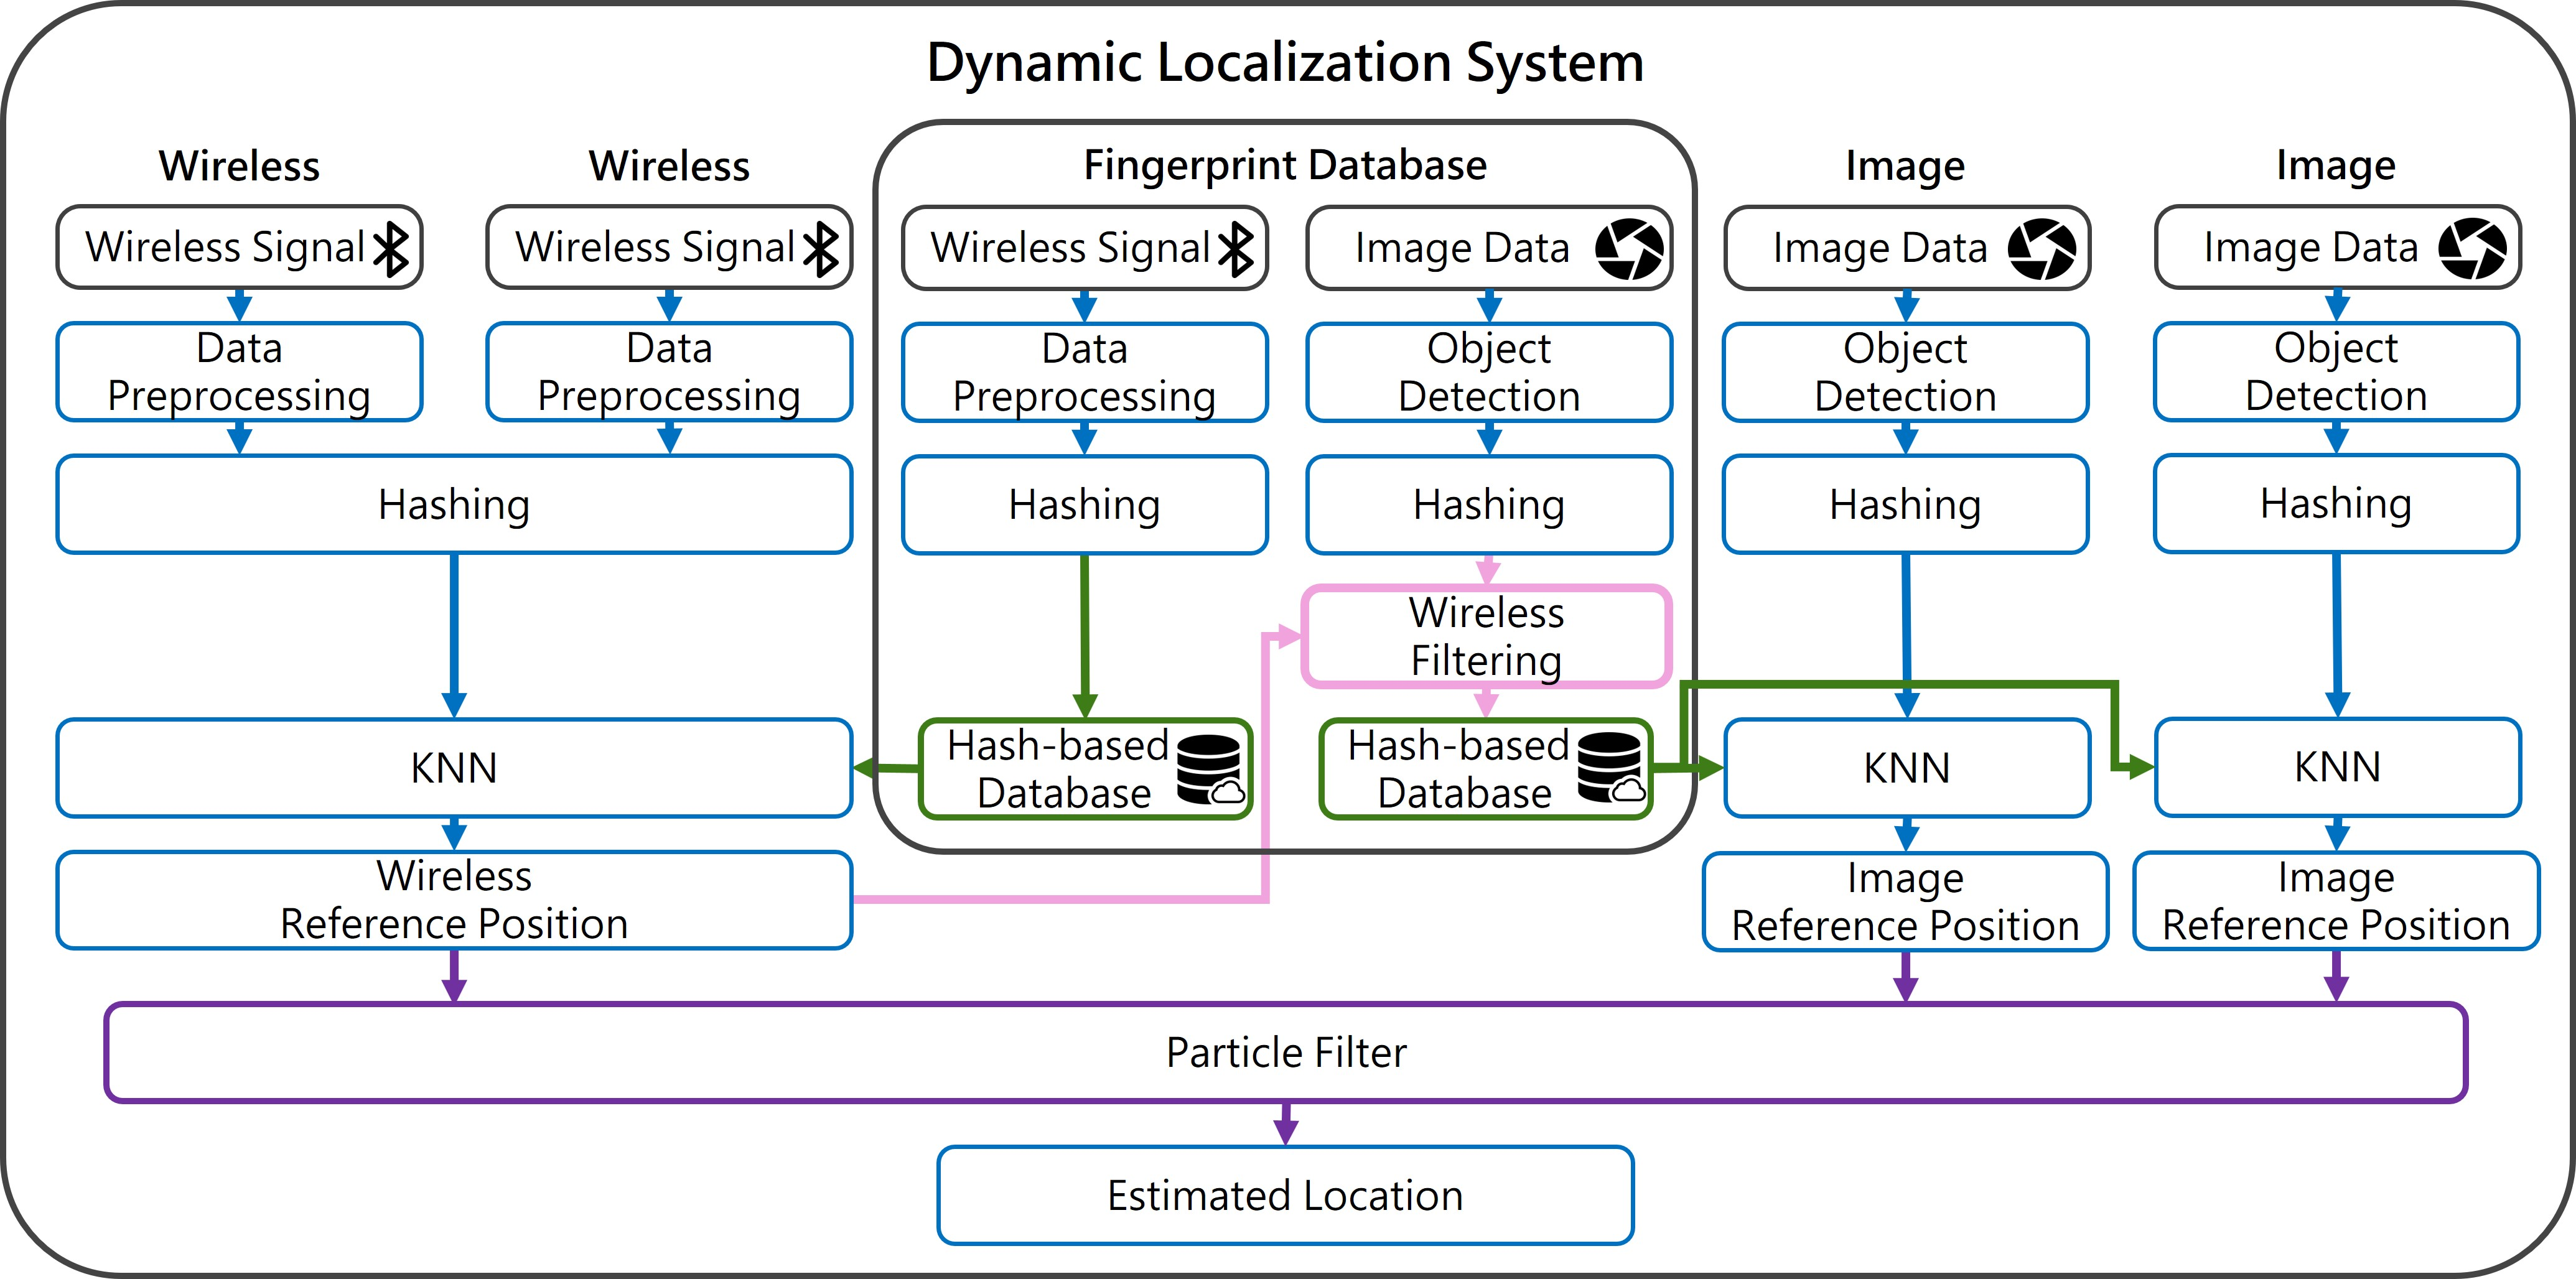
\includegraphics[width=0.95\textwidth]{images/3_Dynamic_Localization_System.jpg}
    \caption{Dynamic Localization System architecture.}
    \label{figure:3_Hierarchical_Localization_System}
    \end{center}
\end{figure}
% === figure === %

%*----------------------section 3.1
\section{Fingerprint Database}

\paragraph{}
Before localization, the detailed information of each positioning point in the environment will be recorded for each new experimental environment, including the RSSI of the wireless signal and the image data of the 360-degree viewing. These collected data will be stored in the database, and will be read and compared during each testing, which is an indispensable data for the entire localization system.
%

%*----------------------section 3.2
\section{Dynamic Localization System}

\paragraph{}
The core system of this research includes two localization methods, wireless fingerprint and image fingerprint, which are dynamically integrated by particle filter.
%

\paragraph{}
Wireless fingerprint will collect the wireless signal RSSI, through data preprocessing, hashing analysis, and finally complete the positioning; image fingerprint will capture the image data, through object detection, hashing analysis, and finally complete the positioning. In the positioning stage, wireless fingerprint and image fingerprint seem to run independently, but in fact, wireless filtering is added to maximize the positioning performance of the two at different spatial scales. Finally, the wireless and image positioning results are imported into the particle filter in a real-time dynamic weighting manner, so that the data obtained by the particle filter can adapt to the rapid changes in the environment. Particle filter is used to integrate past positioning information, so that the positioning of the system is continuous, ensuring that each positioning will not have a large deviation. After the integration of particle filter, the Dynamic Localization System is completed.
%

%*----------------------section 3.3
\section{Wireless Phase}

\paragraph{}
Wireless phase analyzes the RSSI of wireless signal from different beacons in the environment for each testing point $p_t^w$. The device will have similar RSSI of wireless signal at similar points, so by comparing the RSSI received by the device during the test with the RSSI in the database, the similarity calculated by the two can be used for the positioning. In this study, we propose to convert different wireless beacons and their corresponding RSSI at each point into hashing as a comparison for fingerprint.
%

%*----subsection 3.3.1
\subsection{Data Preprocessing and Enhancing}

\paragraph{}
We use multiple devices to collect wireless signals from different beacons, so we consider chip differences and device heterogeneity among different devices. We use Min-Max normalization to normalize the collected RSSI to eliminate the RSSI differences due to device differences. And to avoid the distribution of RSSI values at different distances from being too concentrated, we use Polynomial Enhancing to make the RSSI values at different distances more discrete to facilitate subsequent positioning.
%

\subsubsection{Min-Max Normalization}
\paragraph{}
We use the formula as shown in (\ref{equation:Min-Max_Normalization}) to do Min-Max normalization, where $RSSI_{max}$ is the maximum RSSI collected in the environment, $RSSI_{min}$ is the minimum RSSI collected in the environment, We do Min-Max normalization for each $RSSI_i$ value collected, and the normalized $RSSI_i^{'}$ value is between 0 and 1. We send the normalized $RSSI_i^{'}$ value to the next stage Polynomial Enhancing for use.
%---
\begin{equation}
\label{equation:Min-Max_Normalization}
{RSSI}_i^{'}=\frac{{RSSI}_i-{RSSI}_{min}}{{RSSI}_{max}-{RSSI}_{min}}
\end{equation}
%---

\subsubsection{Polynomial Enhancing}
\paragraph{}
Because the relationship between the RSSI value and the distance is an exponential relationship rather than a linear relationship, the difference change in the RSSI value will become smaller and smaller as the distance increases, and the distance difference cannot be correctly distinguished in the subsequent hashing stage.
%

\paragraph{}
Therefore, we propose the formula as shown in (\ref{equation:Polynomial_Enhancing}) to do Polynomial Enhancing, in which the parameter $a_n$ can be adjusted according to the objective environment and device, and $x$ is the $RSSI_i^{'}$ value after Min-Max normalization in the previous section. The $RSSI_i^{''}$ obtained through Polynomial Enhancing can not only disperse the RSSI value that is too concentrated, but also emphasize the RSSI value that is closer to the beacon. We send the $RSSI_i^{''}$ value after polynomial enhancing to the next stage of hashing as the weight of each hash.
%---
\begin{equation}
\label{equation:Polynomial_Enhancing}
RSSI_i^{''} = f_(x) = a_0 x^0 + a_1 x^1 + a_2 x^2 + ...... + a_n x^n , \;\;\;\;\; x= RSSI_i^{'}
\end{equation}
%---

%*----subsection 3.3.2
\subsection{Hashing}

\paragraph{}
Since each point will collect multiple beacons and their corresponding RSSI values during the testing phase and fingerprint database creation, in order to efficiently compare such complex data, this study proposes to use hashing for comparison to positioning. This section will explain in detail how to convert the different wireless beacons of each point and their corresponding RSSI into hash code for the next section to compare the reference position $R_p^{w}$.
%

\paragraph{}
The detailed conversion process is shown in Fig.~\ref{figure:3_3_Wireless_Hash}. First, at each single testing point $p_t^w$, $n$ beacon IDs are sequentially converted into groups of text hash codes. Because the input beacon IDs are text data, $BLAKE2b$ \cite{Aumasson2013BLAKE2} is selected as the conversion function. Then set the 0 of the text hash code as a negative number and 1 as a positive number, and multiply it with the corresponding $RSSI_n^{''}$ after data preprocessing and enhancing in the previous section to obtain $n$ groups of weighting hashes. Then add up the weighting hashes processed by $n$ groups of different beacons to obtain a group of aggregation hashes composed of positive and negative numbers. Finally, the aggregation hash is signed encoding to a set of wireless hash $h_t^{w}$ composed of 0 and 1 through its positive and negative relationship.
%

\paragraph{}
At each testing point $p_t^w$, there is a set of wireless hash $h_t^{w}$ consisting of beacons and their corresponding RSSI value, and this set of wireless hash ($h_t^{w}$) will provide the next section to find the reference position.
%

\subsection{Multi-device Integration}
\paragraph{}
In the case of multi-device localization, we need to integrate aggregation hash from different devices. The aggregation hash contains the features of multiple beacons in different devices and their corresponding RSSI values. Therefore, the aggregation hashes corresponding to these devices are added together to obtain a set of aggregation hashes composed of multiple devices. This group of multi-device aggregation hash integrates information between different devices, and finally the aggregation hash is signed encoding into a set of wireless hash $h_t^{w}$ composed of 0 and 1 through its positive and negative relationship.
%

%=== figure 3_3_Wireless_Hash=== %
\begin{figure}[tbph]
    \begin{center}
    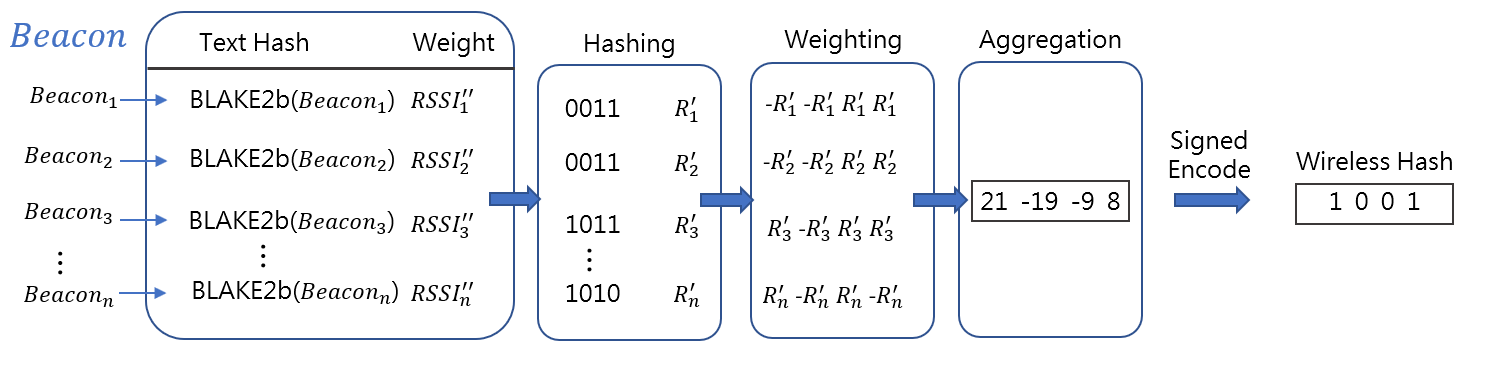
\includegraphics[width=0.95\textwidth]{images/3_3_Wireless_Hash.png}
    \caption{Wireless hashing overview.}
    \label{figure:3_3_Wireless_Hash}
    \end{center}
\end{figure}
% === figure === %

%*----subsection 3.3.3
\subsection{Wireless KNN}

\paragraph{}
Because the devices will have similar wireless signal RSSI groups at similar points, and similar RSSI groups will have similar wireless hash $h^{w}$ through the conversion of hashing in the previous section. The higher the similarity of the wireless hash $h^{w}$, the closer the actual physical distance is. Therefore, by comparing the wireless hash $h_t^{w}$ of the device during testing with the wireless hash $h_b^{w}$ in the database, the correct positioning point during testing can be found. This section will discuss how to calculate the similarity of wireless hash between the test set $h_t^{w}$ and the database $h_b^{w}$.
%

\subsubsection{Position Similarity}
\paragraph{}
Two groups of similar wireless hash ($h_t^{w}$, $h_b^{w}$) have similar hamming distances. Therefore, the similarity can be obtained by calculating the Hamming Distance between the two sets of wireless hash ($h_t^{w}$, $h_b^{w}$). The similarity calculation formula is shown as
%---
\begin{equation}
\label{equation:wireless_position_similarity}
Wireless\ Position\ Similarity(p_t^w, p_b^w) = 1 - \frac{Hamming\ Distance(h_t^w, h_b^{w})}{\left|h_t^w\right|}
\end{equation}
%---
where $\left|h_t^w\right|$ means the number of bits of $h_t^w$.

\subsubsection{Wireless Reference Position}
\paragraph{}
The higher the position similarity calculated in the previous step, the closer the actual physical distance is. In order to avoid extracting extreme values, the database positions $p_b^w$ of top $K_w$ position similarity calculated in the previous step are stored in the wireless reference positions $r_{set}^{w}$. The wireless reference positions $r_{set}^{w}$ will be output to the subsequent particle filter as the basis for particle update.
%

\paragraph{}
Finally, we find the most frequent element from the wireless reference positions $r_{set}^{w}$ as the wireless reference position $R_p^{w}$ of the wireless phase, and use it as the judgment basis for the subsequent wireless filtering and dynamic weighting.
%

%*----------------------section 3.4
\section{Image Phase}

\paragraph{}
Image phase analyzes the object features in the image data of each testing point $p_t^i$. The images seen by the device at similar points will have similar object features, including the object type, object size, and object position in the image. Therefore, by comparing the object features collected by the device during the test with the object features in the database, the similarity calculated by the two can be used for the positioning. In this study, we propose to convert different object types and their corresponding sizes and positions at each point into hashing as a comparison for fingerprint.
%

%*----subsection 3.4.1
\subsection{Object Detection}

\paragraph{}
To get the object features in the image data, we use YOLOv4 \cite{Bochkovskiy2020YOLOv4} as a tool for object detection. After each image passes through the object detection of YOLOv4, the type, size, and position of each object in the image will be obtained. We will use this as the basis for subsequent hashing. Fig.~\ref{figure:3_4_YOLOv4_Object_Detection} shows an example of object detection result.

%=== figure 3_4_YOLOv4_Object_Detection=== %
\begin{figure}[tbph]
    \begin{center}
    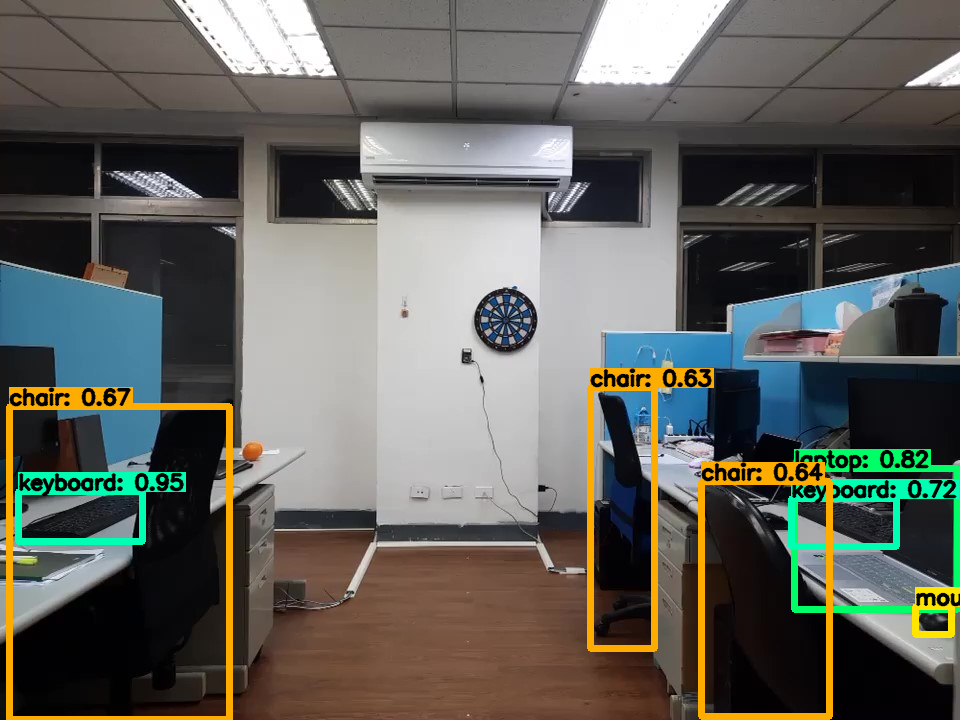
\includegraphics[width=0.65\textwidth]{images/3_4_YOLOv4_Object_Detection.png}
    \caption{ An example of object detection result.}
    \label{figure:3_4_YOLOv4_Object_Detection}
    \end{center}
\end{figure}
% === figure === %

%*----subsection 3.4.2
\subsection{Hashing}

\paragraph{}
During the testing phase and fingerprint database creation, each point will collect image data from different devices in multiple directions. After the object detection in the previous section, there will be multiple data of object types, object sizes, and object positions in each image. In order to efficiently compare such complex data, this study proposes to use hashing for alignment to complete positioning. This section will explain in detail how to convert different object data in each image in multiple directions at each point into hash code for the next section to compare the reference position $R_p^{i}$.

\paragraph{} 
The detailed conversion process is shown in Fig.~\ref{figure:3_4_Image_Hash}. First, at each single testing point $p_t^i$, $n$ object labels are sequentially converted into $n$ groups of text hash codes through the $BLAKE2b$ function. Then set the 0 of the text hash code as a negative number and 1 as a positive number, and multiply it with the corresponding object size to obtain $n$ groups of weighting hashes. Then add up the weighting hashes processed by $n$ groups of different object labels to obtain a group of aggregation hashes composed of positive and negative numbers. Finally, the aggregation hash is signed encoding to a set of image hash $h_t^{i}$ composed of 0 and 1 through its positive and negative relationship.
%

\paragraph{} 
Each device has a set of image hash $h_t^{i}$ at each testing point $p_t^i$ including the information of object labels, object size and object position, and this set of image hash $h_t^{i}$ will provide the next section to find the reference position $R_p^{i}$.
%

%=== figure 3_4_Image_Hash=== %
\begin{figure}[tbph]
    \begin{center}
    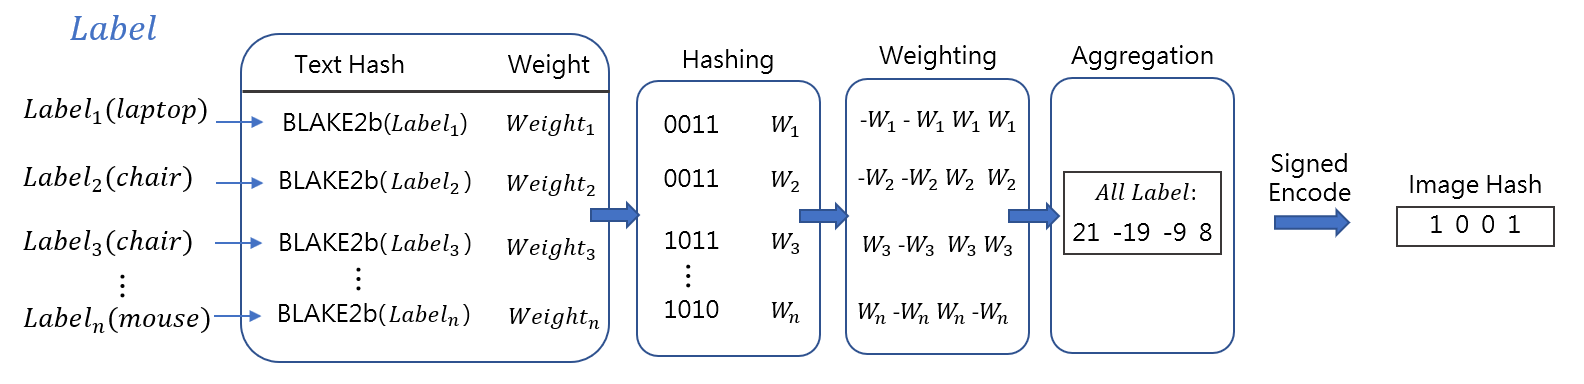
\includegraphics[width=0.95\textwidth]{images/3_4_Image_Hash.png}
    \caption{Image hashing overview.}
    \label{figure:3_4_Image_Hash}
    \end{center}
\end{figure}
% === figure === %

%*----subsection 3.4.3
\subsection{Image KNN}

\paragraph{}
Because the devices will have similar image data sets at similar points, and similar image data will have similar image hash $h^{i}$ through the conversion of hashing in the previous section. The higher the similarity of the image hash $h^{i}$, the closer the actual physical distance is. In addition, we use wireless filtering to limit the scope of the image database, thereby improving the positioning accuracy of image hash.
%

\paragraph{}
By comparing the image hash $h_t^{i}$ of the device during testing with the image hash $h_b^{i}$ in the database, the correct positioning point during testing can be found. This section will discuss how to calculate the similarity of image hash between the test set $h_t^{i}$ and the database $h_b^{i}$.
%

\subsubsection{Wireless Filtering}
\paragraph{}
We found that wireless and image have different positioning performances at different spatial scales. Wireless hash can well locate the approximate range of the user in the large-scale environment, but can not locate the precise position of the user; the image hash can accurately identify the user’s position in a a small-scale range, but will be affected by the high homogeneity of the environment that the positioning has completely deviated in the large-scale environment.
%

\paragraph{}
Therefore, we first use wireless phase to locate a rough position $R_p^{w}$, and then use $R_p^{w}$ as the center to filter the positioning range of the image to the vicinity of $R_p^{w}$. The image database $p_b^i$ after filter is given by
%---
\begin{equation}
\label{equation:Wireless_Filtering}
Image\ Database\ Position\ p_b^i = \left\{\begin{matrix}Pick,\ if\ Euclidean\ Distance\ (R_p^{w},p_b^i)\ < \ d_f \\Drop,\ otherwise\\\end{matrix}\right.
\end{equation}
%---
where $R_p^{w}$ means the wireless reference position from subsection 3.3.3, $d_f$ means the length used as the filtering.

\paragraph{}
After wireless filtering, the scope of the image database $p_b^i$ has shrunk, and all are in the vicinity of $R_p^{w}$. With wireless filtering, image hash positioning will not cause large-scale positioning errors due to repeated scenes in the environment.

\subsubsection{Position Similarity}
\paragraph{}
Two groups of similar image hash ($h_t^{i}$, $h_b^{i}$) have similar hamming distances. Therefore, the similarity can be obtained by calculating the Hamming Distance between the two sets of image hash ($h_t^{i}$, $h_b^{i}$). The similarity calculation formula is shown as
%---
\begin{equation}
\label{equation:image_position_similarity}
Image\ Position\ Similarity(p_t^i, p_b^i) = 1 - \frac{Hamming\ Distance(h_t^i, h_b^{i})}{\left|h_t^i\right|}
\end{equation}
%---
where $\left|h_t^i\right|$ means the number of bits of $h_t^i$.

\subsubsection{Image Reference Position}
\paragraph{}
The higher the position similarity calculated in the previous step, the closer the actual physical distance is. In order to avoid extracting extreme values, the database positions $p_b^i$ of top $K_i$ position similarity calculated in the previous step are stored in the image reference positions $r_{set}^{i}$. The image reference positions $r_{set}^{i}$ will be output to the subsequent particle filter as the basis for particle update.

\paragraph{}
Finally, we find the most frequent element from the image reference positions $r_{set}^{i}$ as the image reference position $R_p^{i}$ of the image phase, and use it as the judgment basis for the subsequent dynamic weighting.

\subsubsection{Multi-device Integration}
\paragraph{}
In the case of multi-device localization, we need to integrate image data from different perspectives of different devices. Because the more diverse the types of objects identified in the image, the more and more accurate the positioning judgment basis will be. Therefore, the elements in the image reference positions $r_{set}^{i}$ of each devices are multiplied by the number of object types recognized in the image, and integrated into a set of image reference positions $r_{set}^{i}$ with multi-device information. Finally, find the most frequent element from the image reference positions $r_{set}^{i}$ as the Image Reference Position $R_p^{i}$ of the image hash part. 

\paragraph{}
This image reference positions $r_{set}^{i}$ with information of the number of object types will be output to the subsequent particle filter as the basis for particle update, and will be used as the judgment basis for the subsequent Dynamic Weighting.

%*----------------------section 3.5
\section{Particle Filter}

\paragraph{}
Our particle filter is referred to the particle filter in \cite{Sou2022JoLo, Lin2021}, which is a localization method that considers multi-device and previous localization results. The main difference between particle filter in \cite{Lin2021} and our method is that we also take into account the current positioning performance of wireless and image, and even objective factors such as the environment, to dynamic weighting between wireless hash $r_{set}^{w}$ and image hash $r_{set}^{i}$  for every time particle update.

\subsubsection{Dynamic Weighting}
\paragraph{}
In the whole testing process, the performance of wireless and image is not always the same. The wireless positioning is more accurate near the corners; the more diverse the objects identified in the image, the more accurate the positioning of the image. We dynamically weight the reference positions from wireless hash $r_{set}^{w}$ and image hash $r_{set}^{i}$ into the reference positions $r_{set}^{pf}$ for particle filter. When wireless reference position $R_p^{w}$ is in the corner, reference positions $r_{set}^{pf}$ takes all wireless; when wireless reference position $R_p^{w}$ is not in the corner, the ratio between wireless and image changes with the number of recognized object classes. When there are more classes of objects identified, the higher the proportion of images is. The dynamic weighting between wireless and image is shown as
%---
\begin{equation}
\label{equation:Dynamic_Weighting}
Reference\ Positions\ r_{set}^{pf} = \left\{\begin{matrix}r_{set}^{w},\ if\ R_p^{w}\ is\ in\ corner\\r_{set}^{w} + Class_{object} \cdot r_{set}^{i} ,\ otherwise\\\end{matrix}\right.
\end{equation}
%---
where $r_{set}^{pf}$ means the reference positions for particle update in particle filter, $r_{set}^{w}$ means the wireless reference positions from subsection 3.3.3, $R_p^{w}$ means the wireless reference position from subsection 3.3.3, $Class_{object}$ means the number of object classes detected in a single image, $r_{set}^{i}$ means the image reference positions from subsection 3.4.3.


\subsubsection{Particle Filter}
\paragraph{}
Fig.~\ref{figure:3_5_Particle_Filter} shows the detail of particle filter. Our method consists of the following steps:

\begin{itemize}
\item  Step 1: Initialization. At the beginning of every testing scenarios, we generate numerous particles on the map using a uniform distribution. Each particle contains a coordinate on the map and a weight, it represents a possible user position.
%---
\item  Step 2: Particle Update. After we get reference positions $r_{set}^{pf}$ from Dynamic Weighting. We count the repeated occurrences of each position in reference positions $r_{set}^{pf}$, and update the weight of particles at that position with them. The more occurrences, the more the weight of particles at that location will be.
%---
\item  Step 3: Location Estimation. After particle update with the weight, we add up all particle weights of each position on the map. Finally, select the position $R_{final}^{pf}$ with the largest weight for the last step, Estimated Location.
%---
\item  Step 4: Re-sample. This step generates new particles using the resulting importance weights and adds them to the next iteration.
%---
\end{itemize}
%

%=== figure 3_Hierarchical_Localization_System=== %
\begin{figure}[tbph]
    \begin{center}
    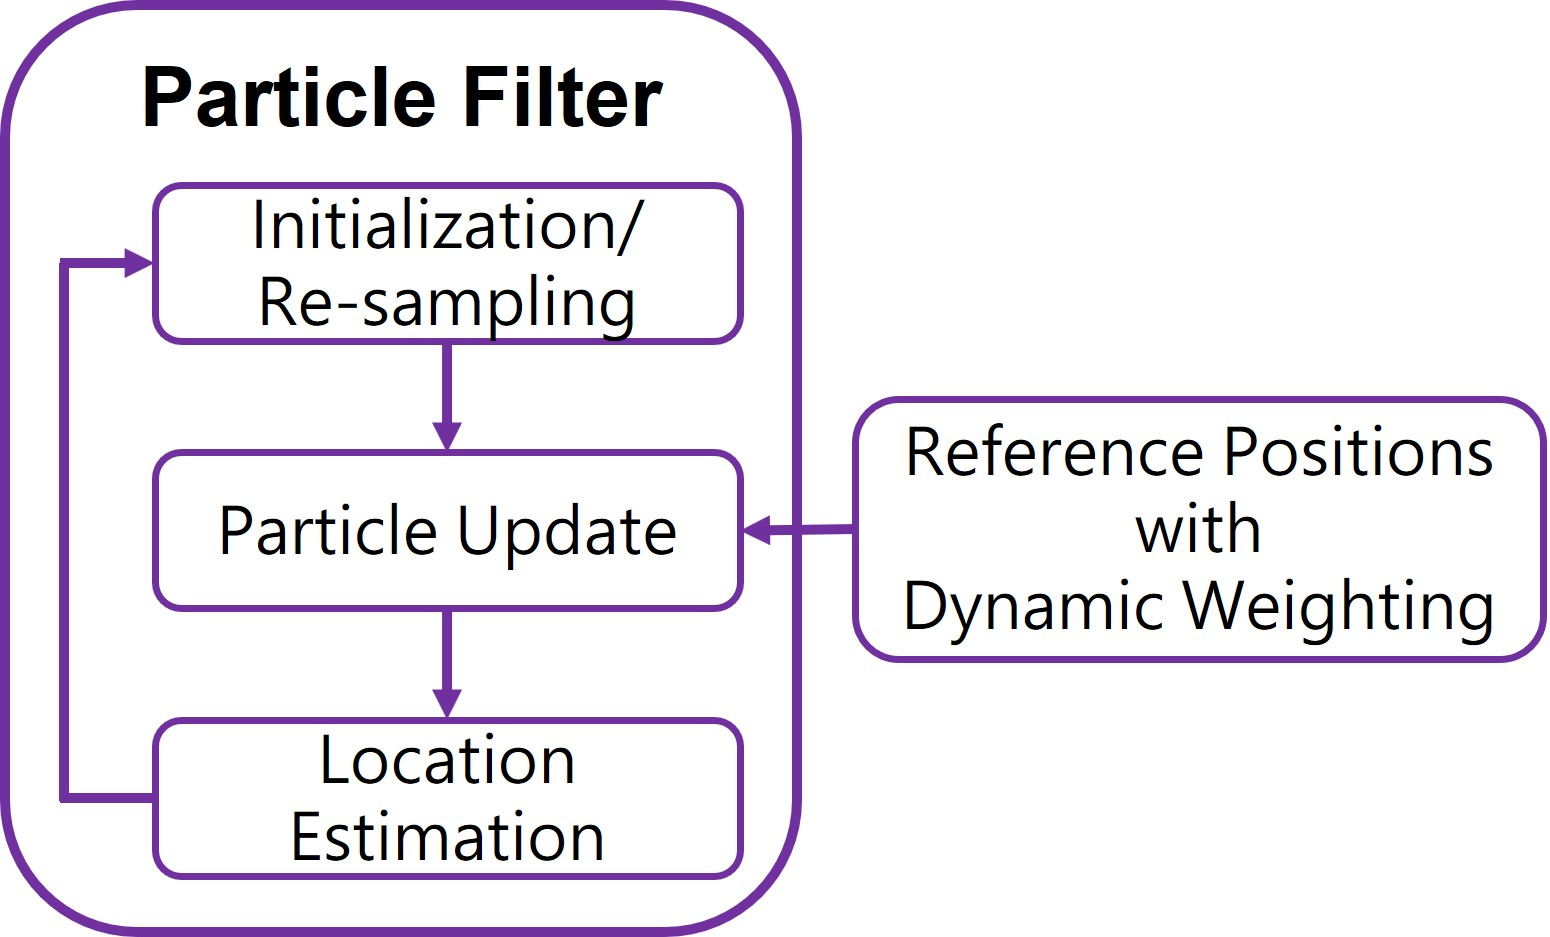
\includegraphics[width=0.8\textwidth]{images/3_5_Particle_Filter.jpg}
    \caption{Particle Filter overview.}
    \label{figure:3_5_Particle_Filter}
    \end{center}
\end{figure}
% === figure === %

%*----------------------section 3.6
\section{Estimated Location}

\paragraph{}
From the beginning, the wireless hash uses the wireless signal to locate and obtain the wireless reference positions $r_{set}^{w}$, the image hash processes the image data to locate and obtain the image reference positions $r_{set}^{i}$, and then integrates the output of the two through dynamic weighting to obtain $r_{set}^{pf}$, finally get $R_{final}^{pf}$ by particle filter. After completing all the processes of the system, $R_{final}^{pf}$ is the positioning result of the entire Dynamic Localization System.
%

%*------------------------------------------------chapter 4-------------------------------------------
\chapter{Experimental Setup}

\paragraph{}
Before actually verifying the performance of our method, this chapter introduces the details and parameters of our experiment in detail, including the mobile device of the experiment, the experimental environment, and the experimental scenarios.

%*----------------------section 4.1
\section{Experimental Devices}

\paragraph{}
In order to use multi-device wireless signal and image data collection, we use 4 mobile phones as experimental devices, as shown in Fig.~\ref{figure:4_1_Experimental_Smartphones}: Samsung A51, hTC U11, hTC U19e, and Sharp V. To allow the mobile phone to accurately capture the image data in four directions, front, back, left, right, and left, we fixed the mobile phone on the holder as shown in Fig.~\ref{figure:4_1_Devices_Holder}, and then placed the device on a tripod 1.2 meters above the ground to simulate the user's hand holding the mobile phone height, and turn the mobile phone outward to collect image data in the front, back, left, and right directions. The mobile phone model and corresponding direction are shown in Table~\ref{table:4_1_Smartphone_Informations}.

%=== figure 4_1_Experimental_Devices=== %
% subfigs for Experimental Smartphones
\begin{figure}[tbph]%\ContinuedFloat
    %\centering
    \begin{subfigure}{1\linewidth}
    \centering
        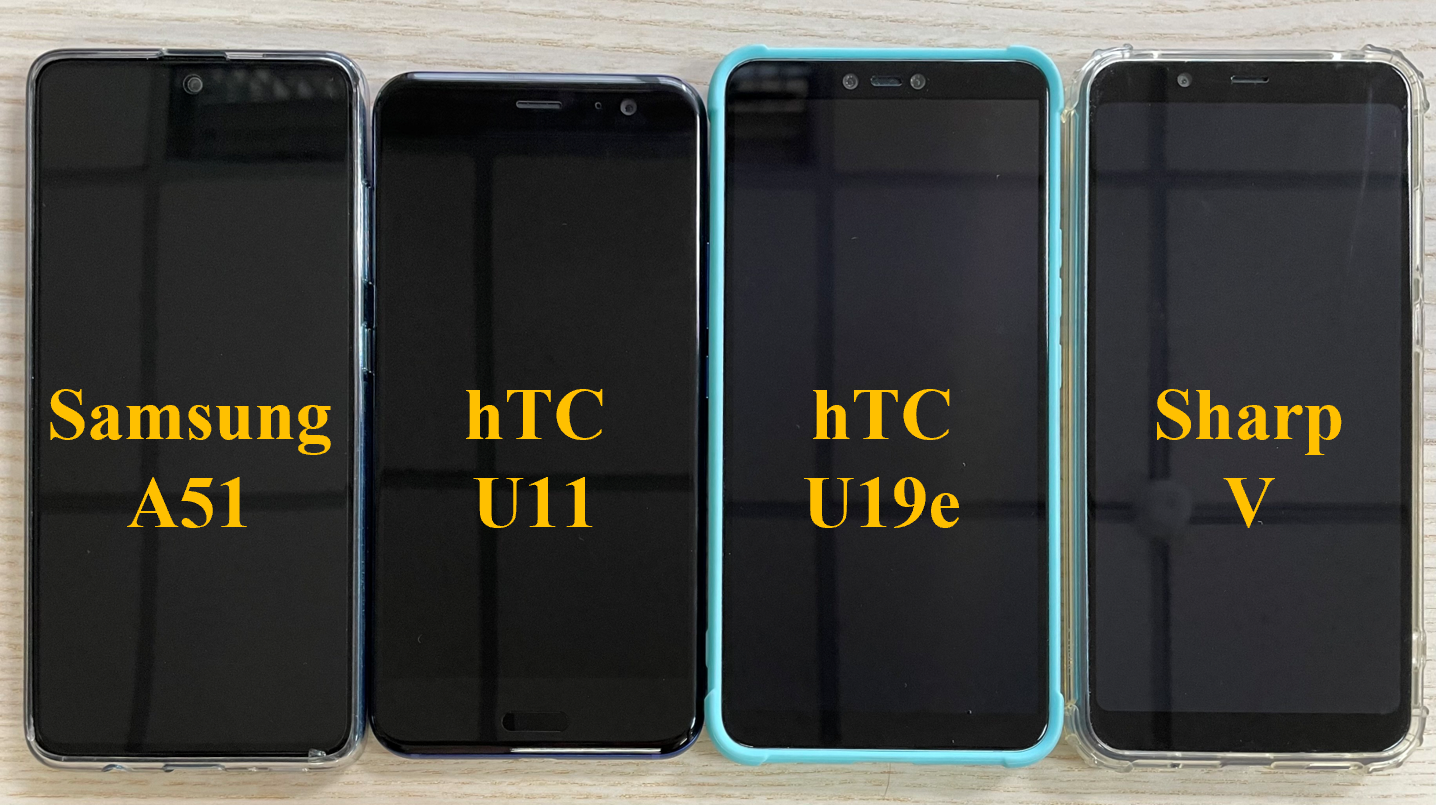
\includegraphics[width=0.8\textwidth]{images/4_1_Experimental_Smartphones.png}
        \caption{Experimental Smartphones}
        \label{figure:4_1_Experimental_Smartphones}
    \end{subfigure}
    %\caption{.}
% subfigs for Devices Holder
    % \centering
    \begin{subfigure}{1\linewidth}
    \centering
        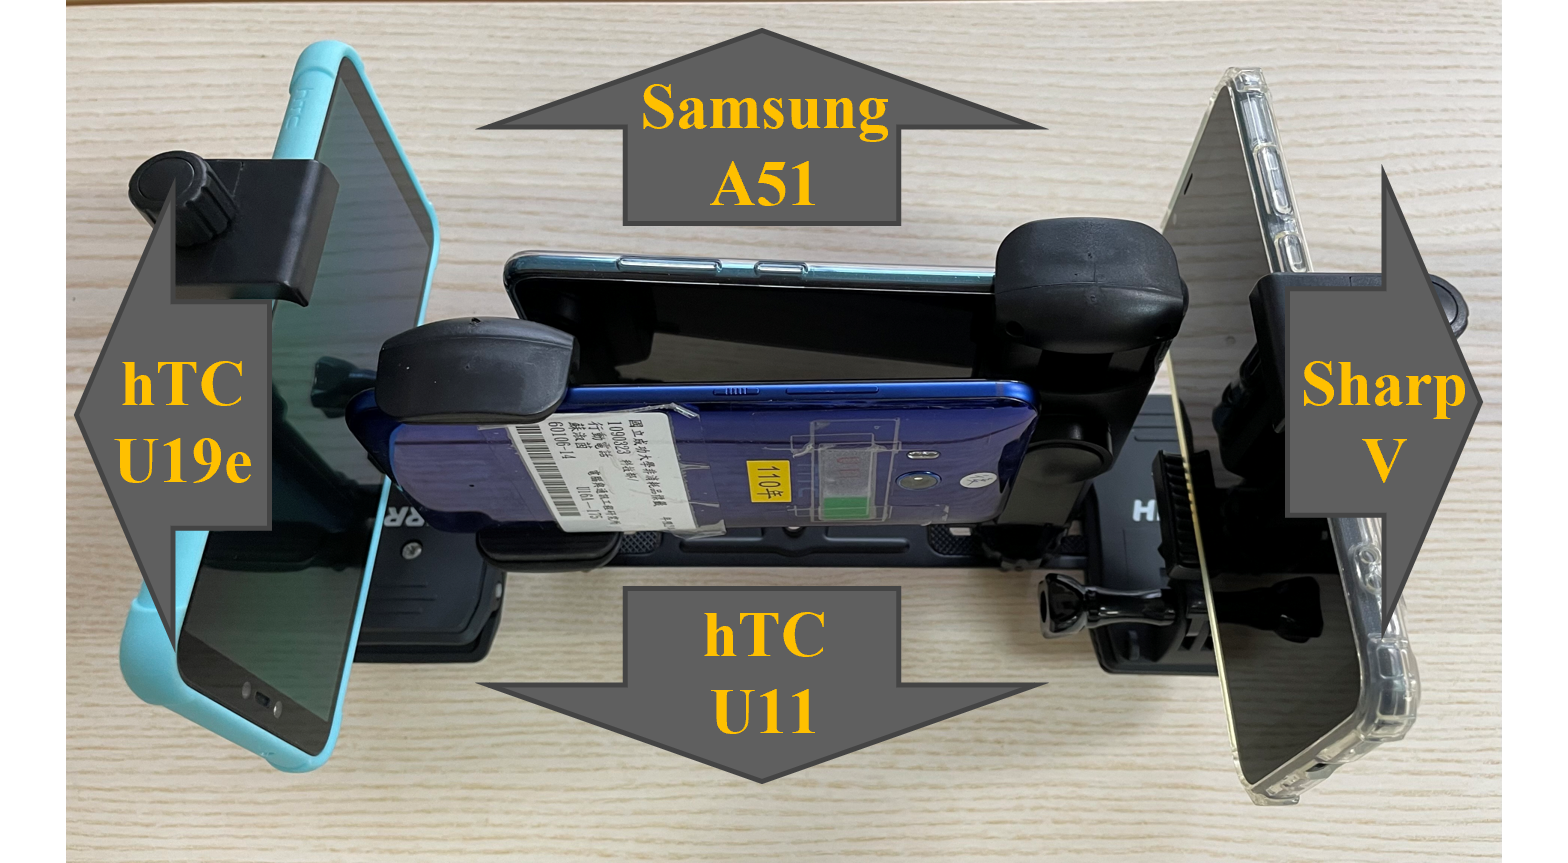
\includegraphics[width=0.8\textwidth]{images/4_1_Devices_Holder.png}
        \caption{Devices Holder}
        \label{figure:4_1_Devices_Holder}
    \end{subfigure}
\caption{Experimental smartphones and devices holder.}
\label{figure:4_1_Experimental_Devices}
\end{figure}
%=== figure === %

% === table === %
\begin{table}
    \begin{center}
    \caption{Information of the smartphones}
    \label{table:4_1_Smartphone_Informations}
        \begin{tabular}{|c|c|c|}
            \hline
                Device & ID as wireless device & Character as camera \\
            \hline
                Samsung A51 & $w_1$ & Front Camera \\
            \hline
                hTC U11     & $w_2$ & Rear Camera \\
            \hline
                hTC U19e    & $w_3$ & Left Camera \\
            \hline
                Sharp V     & $w_4$ & Right Camera \\
            \hline
        \end{tabular}
    \end{center}
\end{table}
% === table === %

%*----------------------section 4.2
\section{Experimental Environment}

\paragraph{}
For the experimental environment, we selected an office environment Room 92589 located in the Electrical Engineering (EE) Department of National Cheng Kung University (NCKU), Tainan, Taiwan. As shown in Fig.~\ref{figure:4_2_Experimental_Environment_picture}, this is an office environment that contains various daily necessities including office desks and chairs, personal computers, keyboards, mice, tablet computers, books, and so on. And the office is a rectangular environment, divided into three rows of aisles by two partitions.

%=== figure 4_2_Experimental_Environment_picture=== %
\begin{figure}[tbph]
    \begin{center}
    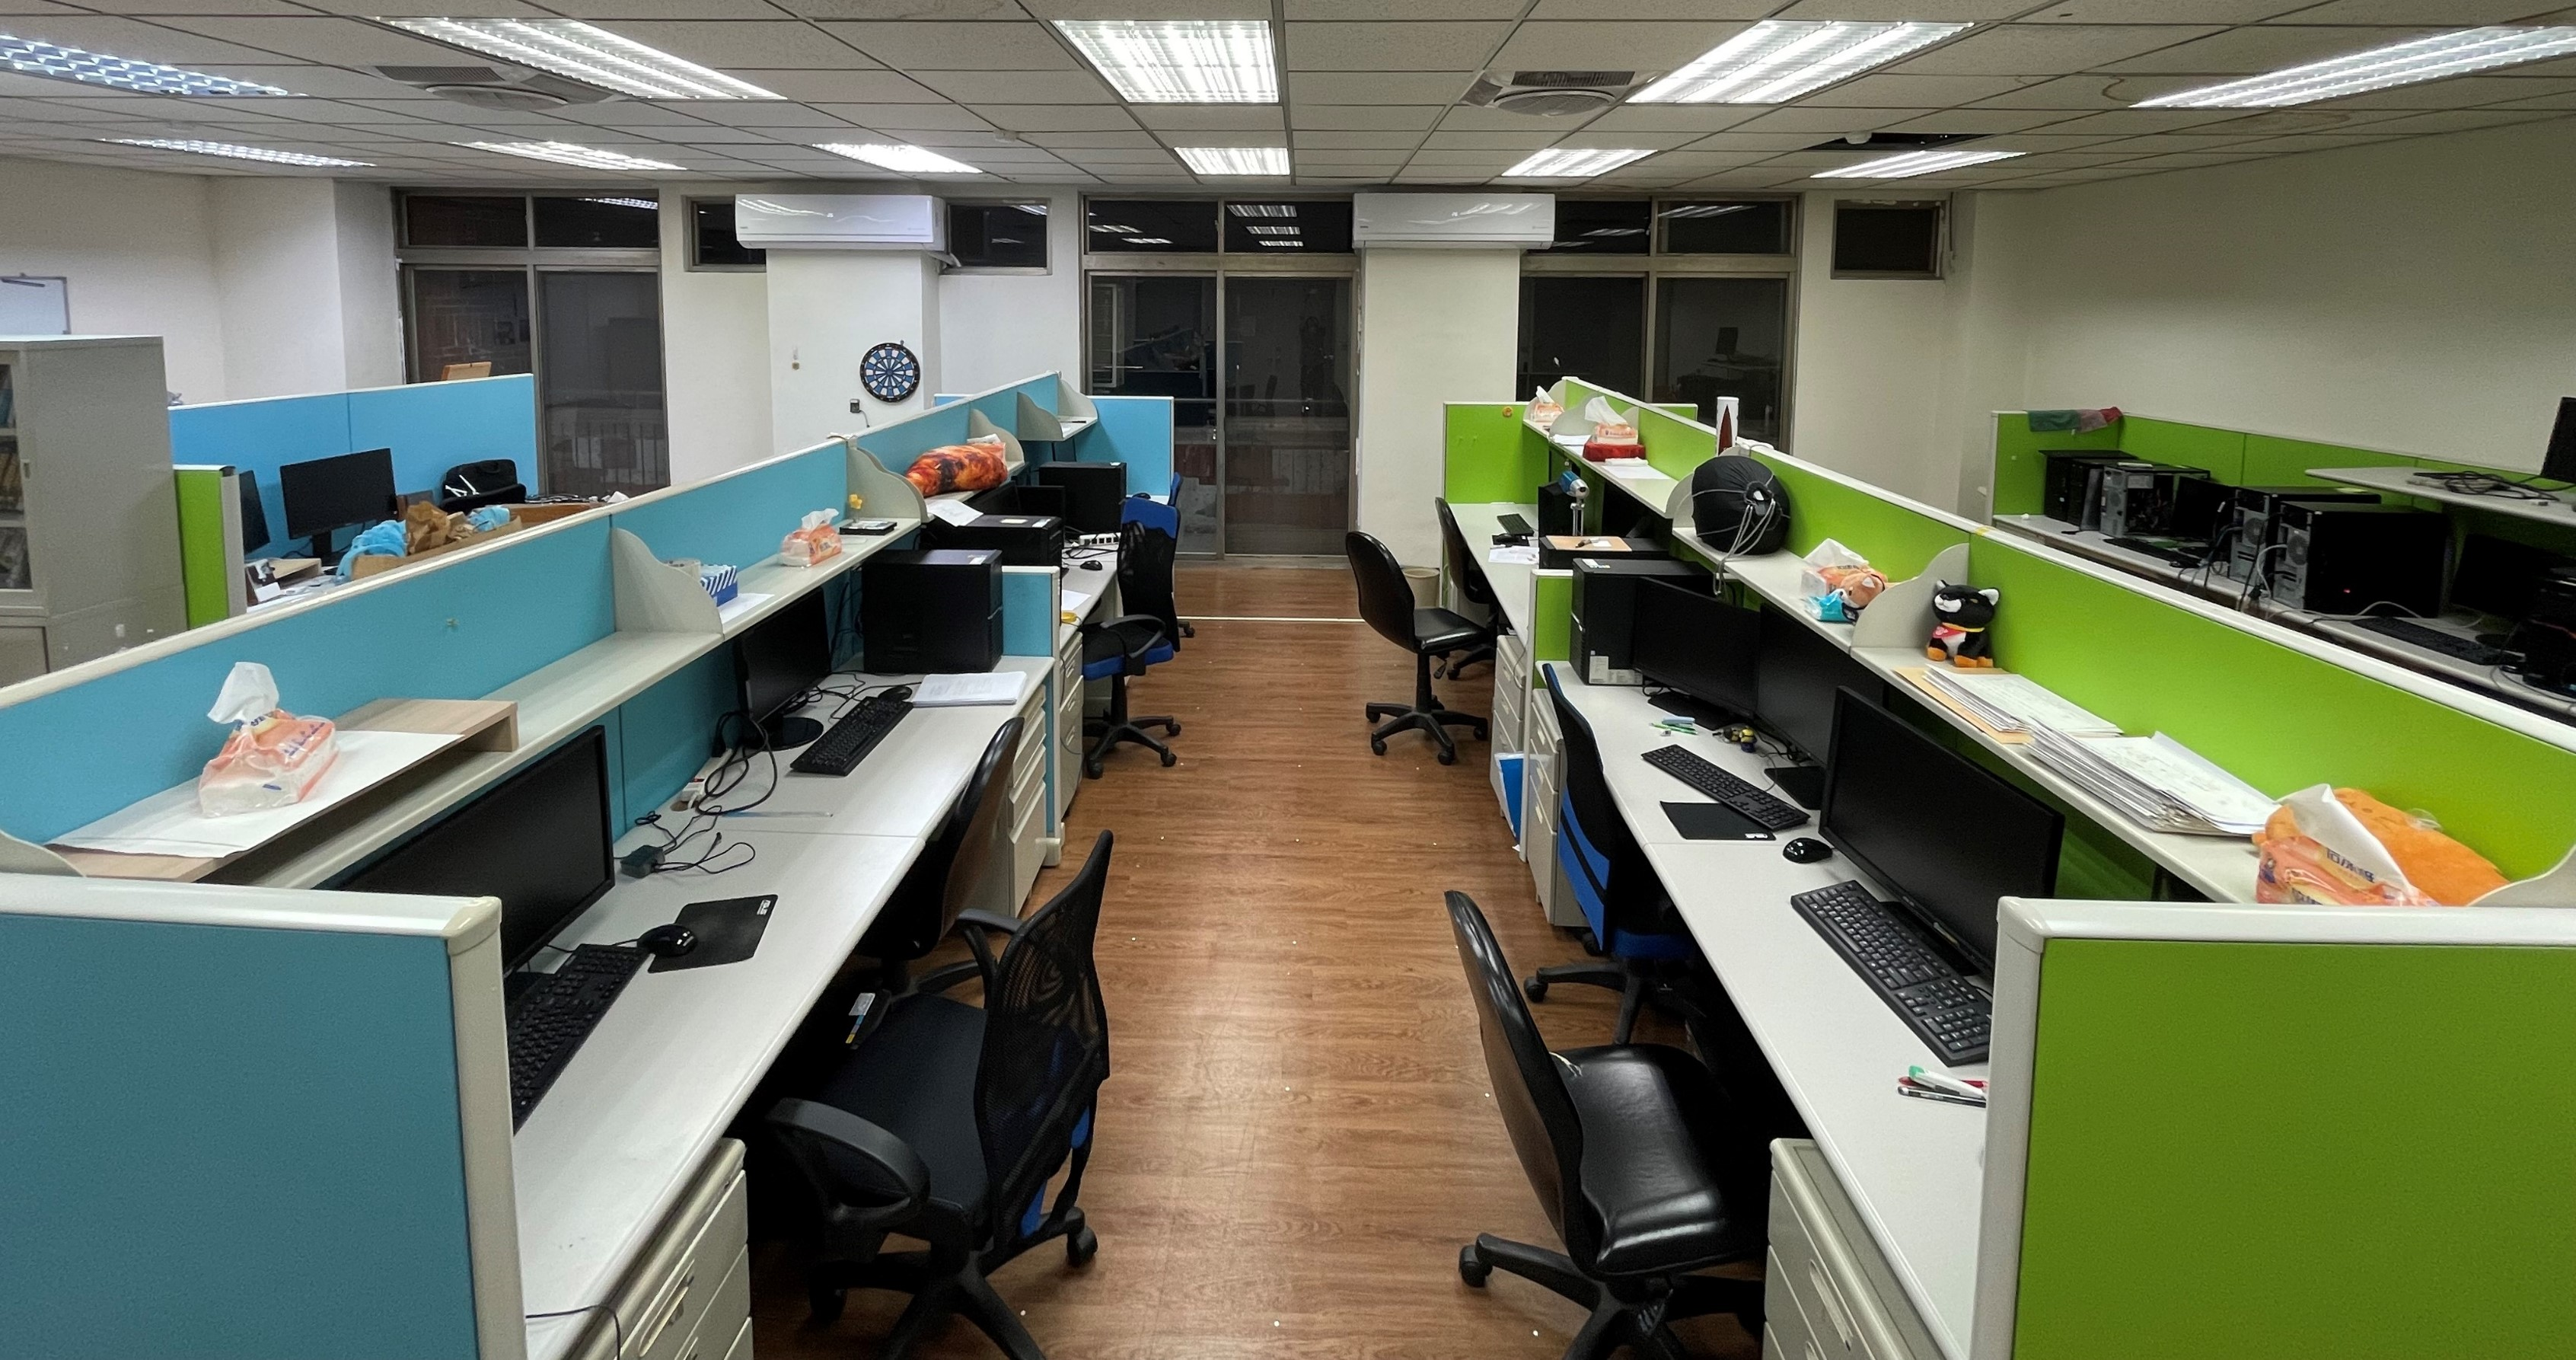
\includegraphics[width=0.8\textwidth]{images/4_2_Experimental_Environment_picture.jpg}
    \caption{Experimental office environment.}
    \label{figure:4_2_Experimental_Environment_picture}
    \end{center}
\end{figure}
% === figure === %

\paragraph{}
We make the space into the floor plan shown in Fig.~\ref{figure:4_2_Experimental_Environment_plan}. We plan a group of M-shaped experimental areas containing 41 positioning points in the remaining aisle space with a length of 6.6 meters and a width of 6.6 meters. And deploy 7 Bluetooth Low Energy (BLE) Beacons made of Raspberry Pi as the wireless signal at a height of 1.2 meters above the ground.
%

%=== figure 4_2_Experimental_Environment_plan=== %
\begin{figure}[tbph]
    \begin{center}
    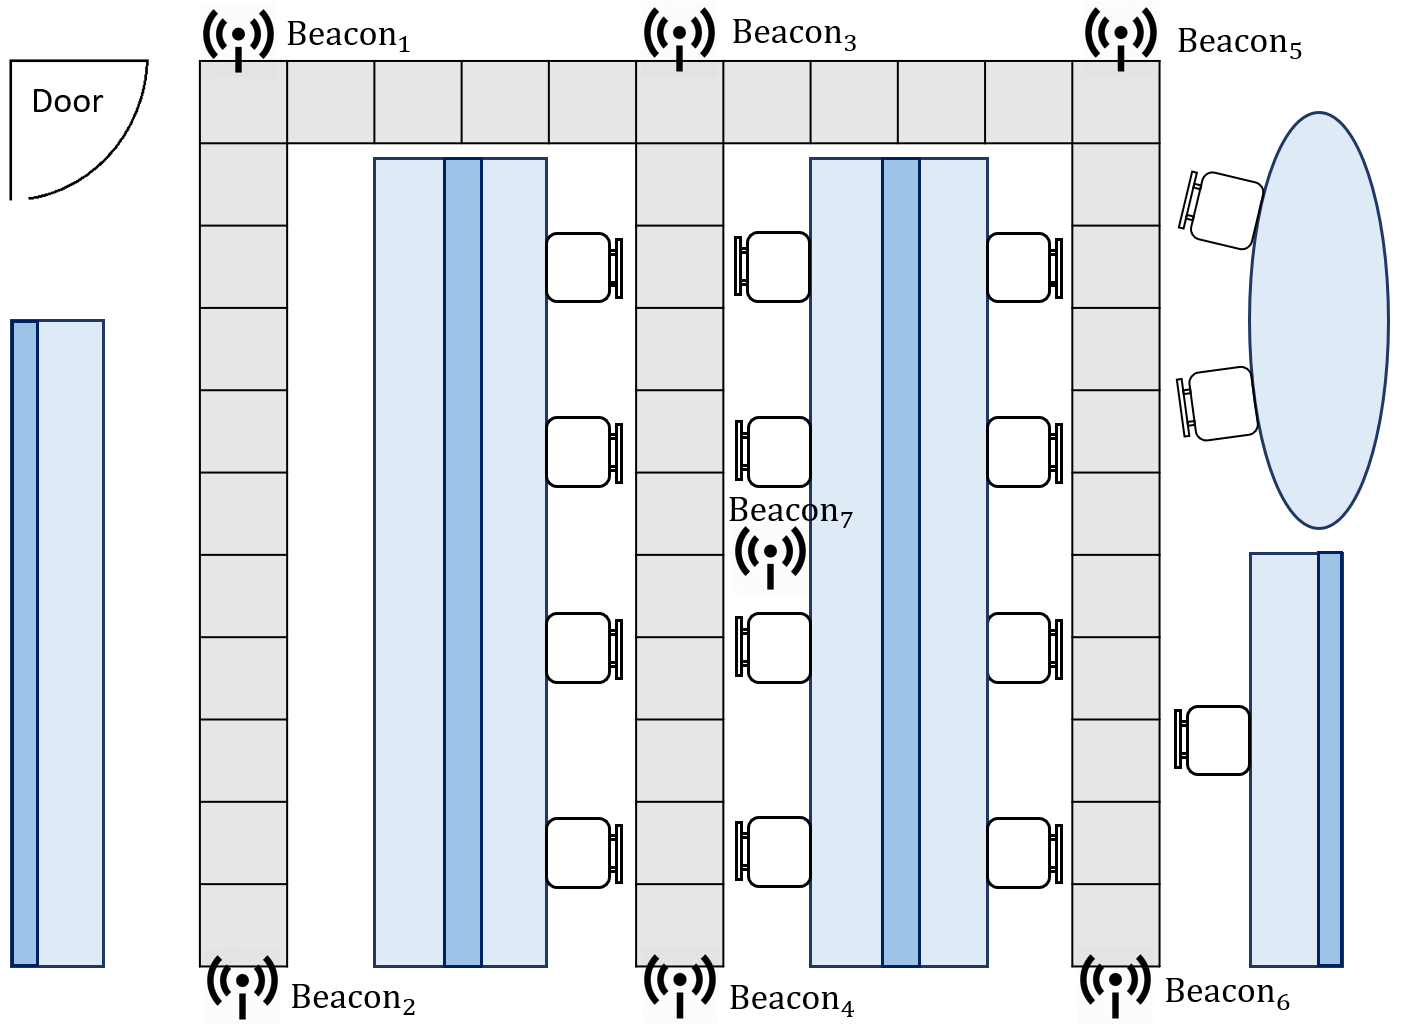
\includegraphics[width=0.8\textwidth]{images/4_2_Experimental_Environment_plan.png}
    \caption{Room plan of the office environment.}
    \label{figure:4_2_Experimental_Environment_plan}
    \end{center}
\end{figure}
% === figure === %

%*----------------------section 4.3
\section{Experimental Scenarios}

\paragraph{}
To evaluate the performance of the system in different dynamics, we plan three different walking scenarios:

\begin{itemize}
\item  Stationary: A stationary fixed point. As shown in Fig.~\ref{figure:4_3_Experimental_Scenarios_ST}, a specific positioning point in the experimental area is selected, and it is stationary. Evaluate the performance of the system at rest.
%---
\item  Scripted Walk: Regular route with regular rate repeating route. As shown in Fig.~\ref{figure:4_3_Experimental_Scenarios_SW}, the tester walks repeatedly at the planned rate according to the planned route to evaluate the performance of the system in such a regular pattern.
%---
\item  Free Walk: Random route with no predetermined route and random speed. There are no restrictions on the tester's route and speed, and they walk exactly as they like. The test subjects can sometimes move quickly, sometimes slowly or even stop, turn left or right randomly or even turn suddenly. It is very challenging to the dynamic modulation capability of the system.
%---
\end{itemize}
%

%=== figure 4_3_Experimental_Scenarios_ST=== %
% subfigs for stationary
\begin{figure}[tbph]%\ContinuedFloat
    %\centering
    \begin{subfigure}{1\linewidth}
    \centering
        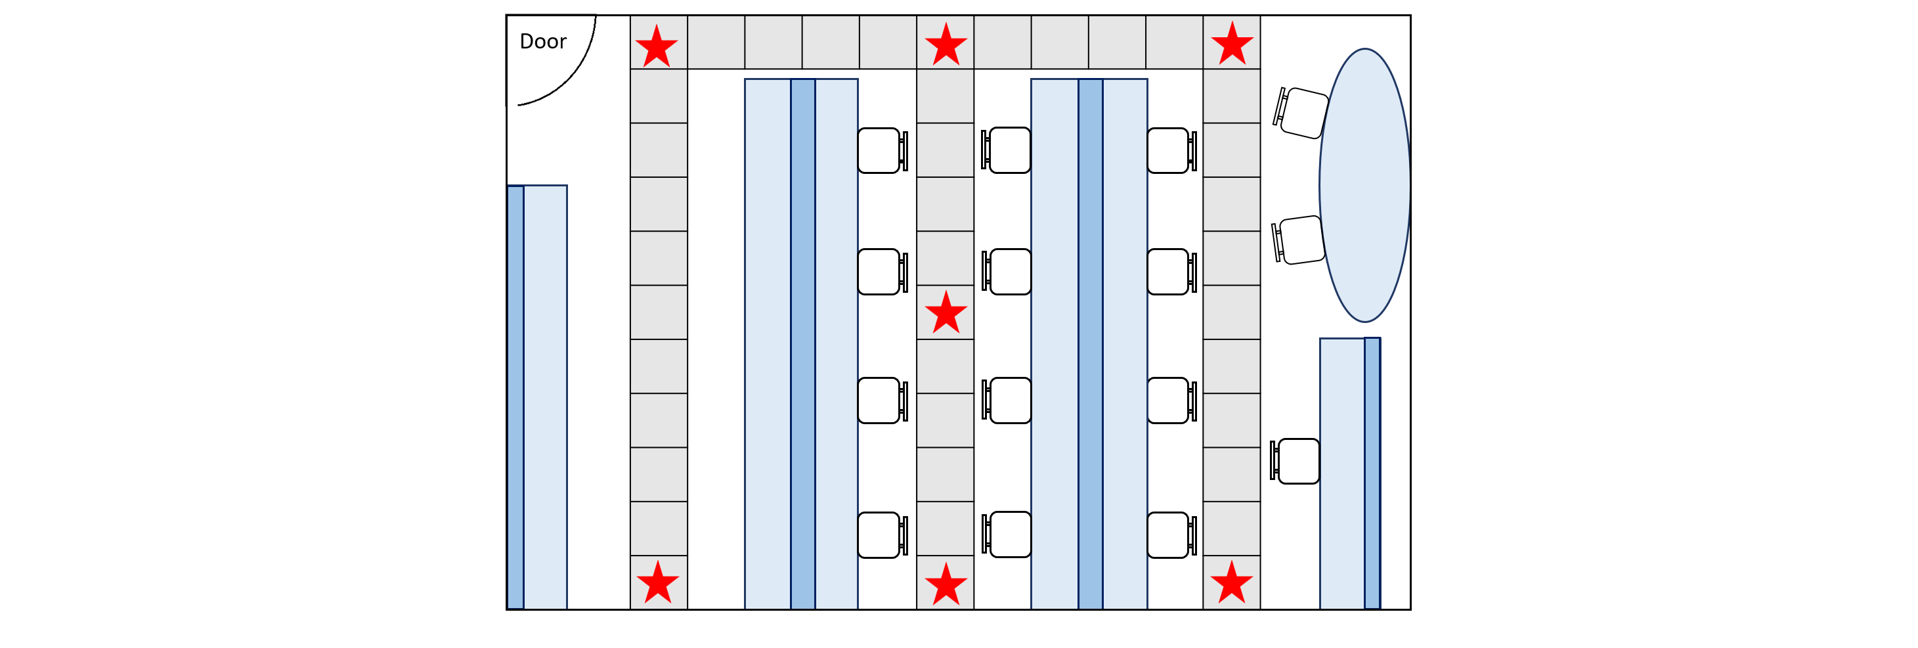
\includegraphics[width=0.85\textwidth]{images/4_3_Experimental_Scenarios_ST.png}
        \caption{Positions of stationary}
        \label{figure:4_3_Experimental_Scenarios_ST}
    \end{subfigure}
    %\caption{.}
% subfigs for scripted walk
    % \centering
    \begin{subfigure}{1\linewidth}
    \centering
        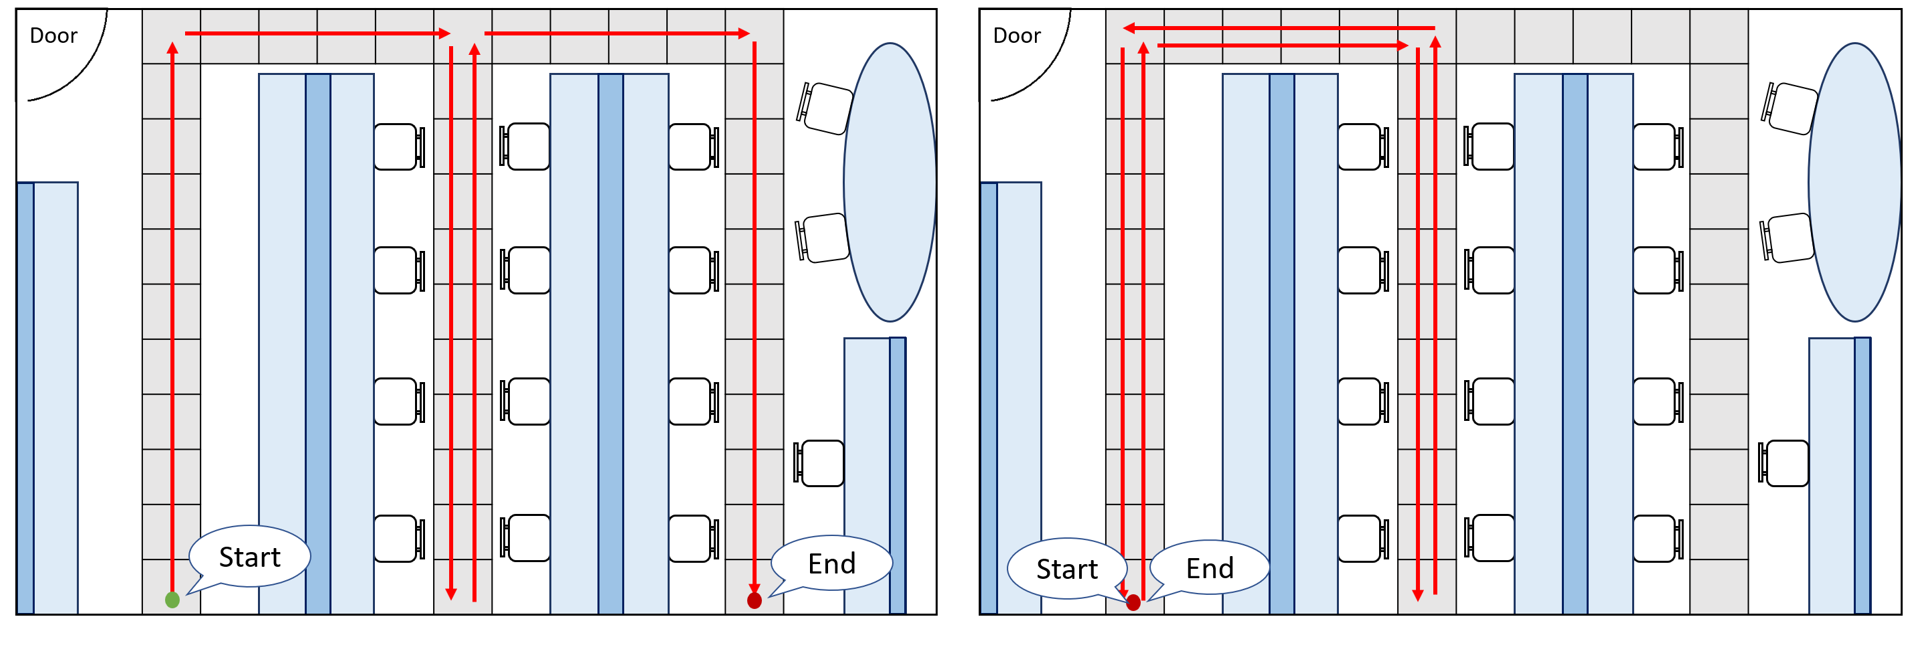
\includegraphics[width=0.85\textwidth]{images/4_3_Experimental_Scenarios_SW.png}
        \caption{Paths of scripted walk}
        \label{figure:4_3_Experimental_Scenarios_SW}
    \end{subfigure}
\caption{Definitions of stationary positions and scripted walk paths.}
\label{figure:4_3_Experimental_Scenarios}
\end{figure}
%=== figure === %

%*----------------------section 4.4
\section{Data Collection}
\paragraph{}
In the training phase, the wireless fingerprint database of the experimental environment is built by collecting 150 wireless fingerprints in average at each positioning point. The image fingerprint database is built by collecting a 360-degree video containing about 900 frames at each positioning point.

\paragraph{}
In the testing phase, each wireless device turned the wireless signals collected every 10 seconds into a wireless fingerprint as wireless testing data at each testing point. And each camera captured a 10 seconds video as image testing data at each testing point.


%*------------------------------------------------chapter 5-------------------------------------------
\chapter{Performance Evaluation}

%paragraph
\paragraph{}
After completing the experimental setup, this chapter is devoted to evaluating the performance of our method. To fairly evaluate system performance, we use mean distance errors (MDEs) and standard
deviation of the distance errors (SDEs), which calculate the distribution of errors, as the performance metrics. The formulas of MDE and SDE are defined as follow:

\begin{equation}
    MDE = \sum_{i}\dfrac{\sqrt{{(x_i-\widehat{x}_i)}^2 + {(y_i-\widehat{y}_i)}^2}}{N}
\end{equation}
\begin{equation}
    SDE = \sqrt{\dfrac{\sum_{i}{(d_i-\bar{d})}^2}{N}}
\end{equation}

Where $x_i$, $y_i$ are the coordinates of the $i$-th estimated position and $\widehat{x}_i$, $\widehat{y}_i$ are the coordinates of corresponding ground truth position, $N$ is the number of testing positions. Then $d_i$ means the distance errors between the $i$-th estimated position and its corresponding ground truth position, $\bar{d}$ is the mean of all $d_i$.

\paragraph{}
In order to comprehensively evaluate our performance, in this chapter we will compare with following three other indoor localization systems :

\begin{itemize}
\item  $BTrack$, a single-device localization system based on wireless signal \cite{Sou2019BTrack} : Compared with the system using single-device wireless signals, we can evaluate how much the indoor localization performance can be improved in our system $DyLo$ when multi-device integration and image data are added.
%---
\item  $JoLo$, a multi-device localization system based on wireless signal \cite{Sou2022JoLo} : Compared with the system using multi-device wireless signals, we can evaluate how much the indoor localization performance can be improved in our system $DyLo$ when the system adds image data to assist positioning.
%---
\item  $Lin$, a multi-device localization system based on wireless and image data \cite{Lin2021}~: Compared with the system using multi-device wireless and image data, we can objectively evaluate how much our system can improve indoor localization performance by the design of dynamic localization system. And because $Lin$ can be integrated between different numbers of devices, we use $L$($w$,$i$) to denote the use of $w$ wireless devices and $i$ image cameras.
%---
\end{itemize}
%

%paragraph 
\paragraph{}
After introducing the three systems for comparison, we will evaluate the performance of our method between the above three systems from the following 8 issues:

\begin{itemize}
\item  Issue 1: Comparisons with other baseline methods. We compare our method against 3 existing indoor localization methods based on wireless signal and image data.
%---
\item  Issue 2: Contribution Between Wireless and Image. To explores the respective contributions of wireless and image to the Dynamic Localization System.
%---
\item  Issue 3: Improvement of data enhancing. To discuss the improvement of data enhancing to wireless signal, $DyLo$ discard image data to compare with $BTrack$ and $JoLo$.
%---
\item  Issue 4: Effects of different environments. To verify that our method is not limited to our office environment, we use another office environment for evaluation.
%---
\item  Issue 5: Effects of the number of cameras and wireless devices. We adjust the number of cameras and wireless devices, and observe the changes in mean distance errors.
%---
\item  Issue 6: Effects of blocked object problem. In order to simulate the situation that some static objects in the environment may be blocked, by ignoring some detected objects in testing data randomly.
%---
\item  Issue 7: Effects of the number of beacons. We reduce the number of beacons to simulate the situation where the environment has fewer beacons, and observe the changes in mean distance errors.
%---
\item  Issue 8: Effects of device heterogeneity. We randomly ignore some BLE packets received by wireless devices to simulate different packet receiving capabilities, and observe the changes in mean distance errors.
%---
\end{itemize}
%

%*----------------------section 5.1
\section{Comparisons with Other Baseline Methods}

\paragraph{}
We compared our system $DyLo$ against 3 existing methods: $BTrack$, $JoLo$, and $Lin$. The mean distance error (MDE) of all scenarios are shown in Fig.~\ref{figure:5_1_Comparisons_with_Other_Methods_MDE}. In the stationary scenario, our system improves the performance of $BTrack$ by at least 95.4\%, improves the performance of $JoLo$ by at least 86.9\%, and improves the performance of $Lin$ by at least 33.3\%. In the scripted walk scenario, our system improves the performance of $BTrack$ by at least 81.6\%, improves the performance of $JoLo$ by at least 66.8\%, and improves the performance of $Lin$ by at least 2\%. And in the free walk scenario, our system improves the performance of $BTrack$ by at least 84.4\%, improves the performance of $JoLo$ by at least 69.5\%, and improves the performance of $Lin$ by at least 34.4\%.

%=== figure 5_1_Comparisons_with_Other_Methods_MDE=== %
\begin{figure}[tbph]
    \begin{center}
    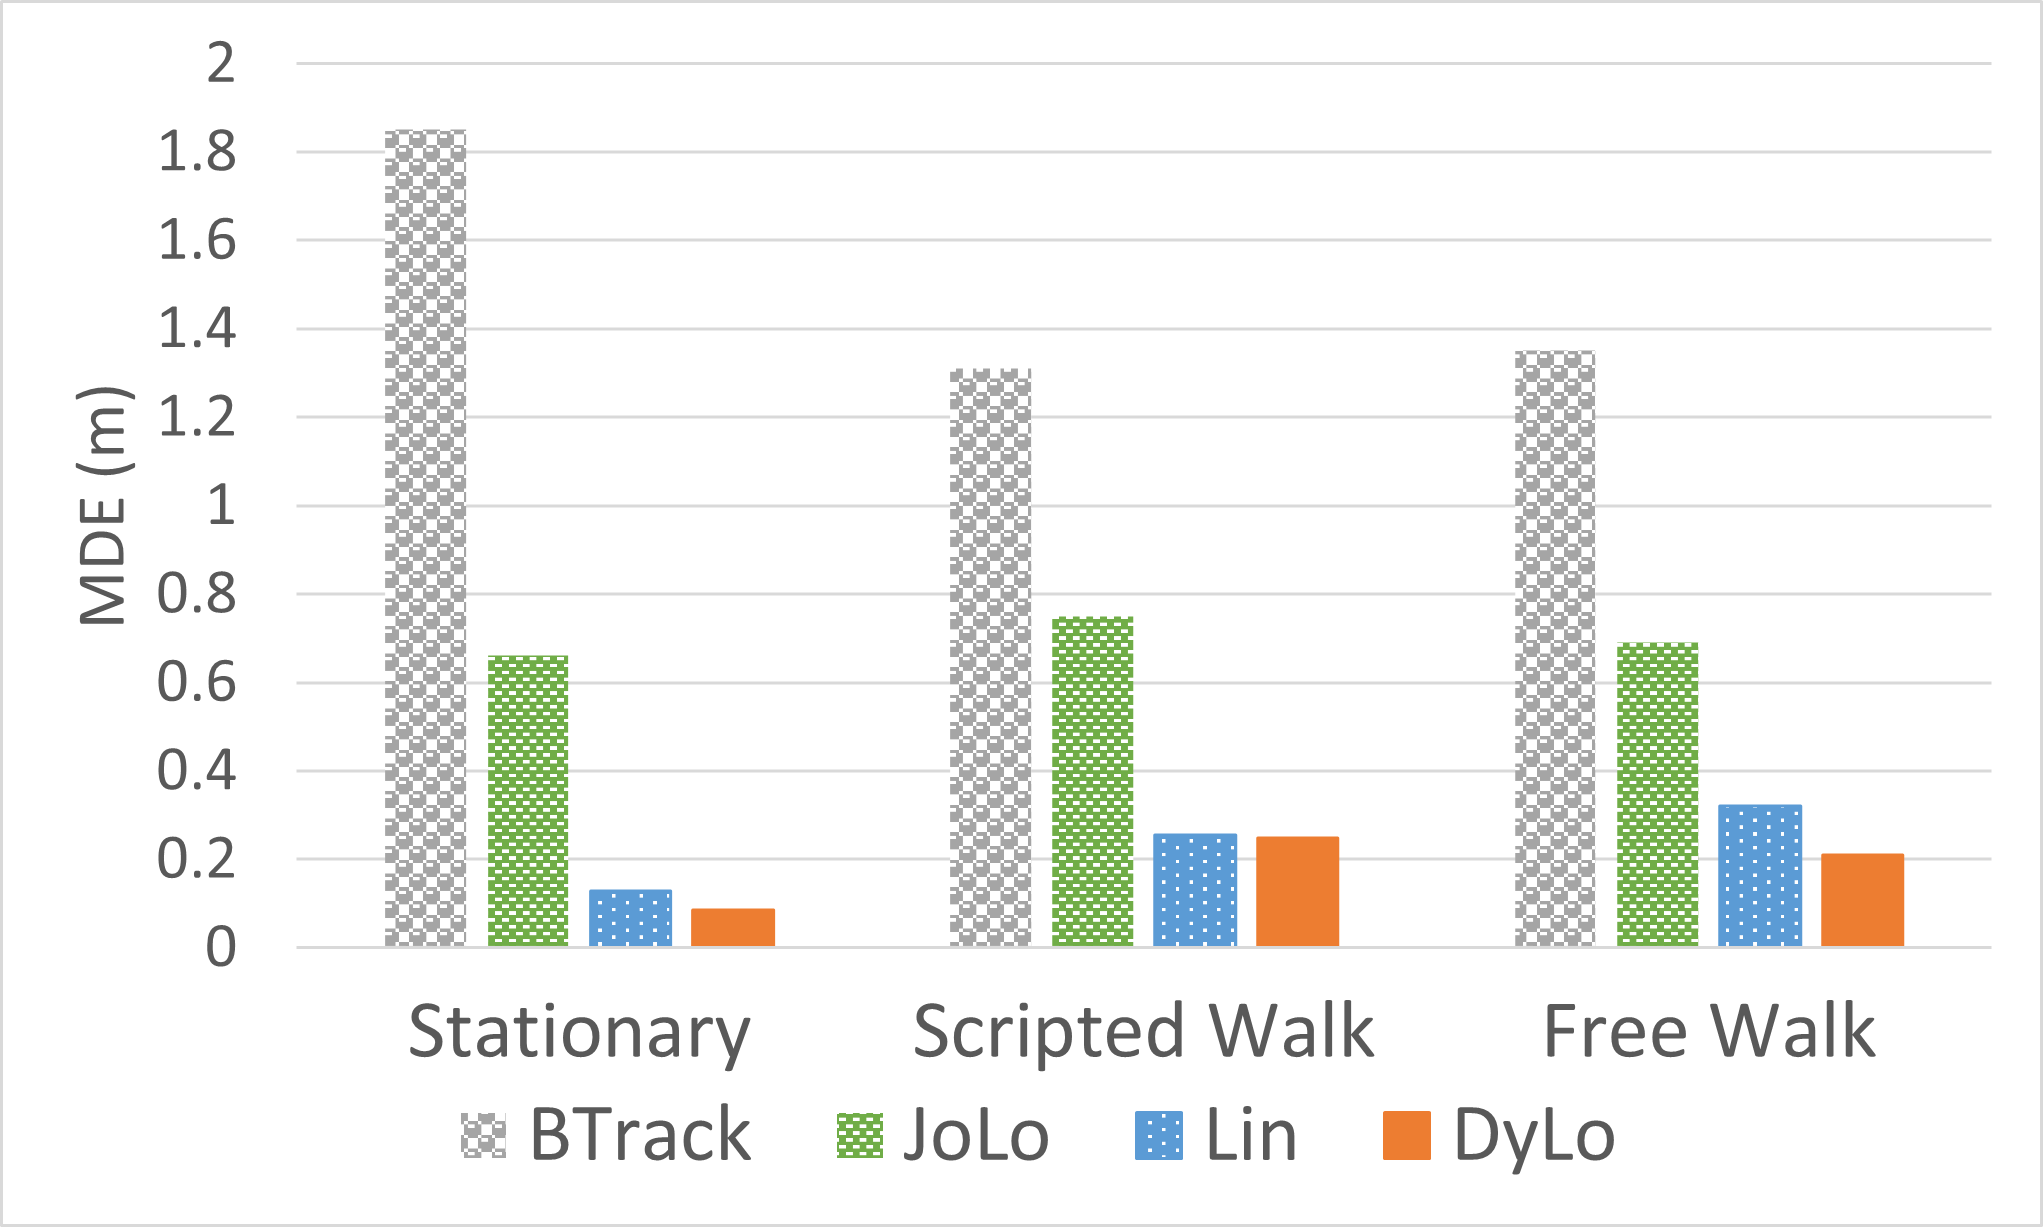
\includegraphics[width=0.8\textwidth]{images/5_1_Comparisons_with_Other_Methods_MDE.png}
    \caption{Comparisons of the MDEs among proposed system and other existing systems.}
    \label{figure:5_1_Comparisons_with_Other_Methods_MDE}
    \end{center}
\end{figure}
% === figure === %

\paragraph{}
Furthermore, we observed the MDE distributions of each method in each scenario. The cumulative distribution function (CDF) of each scenario is shown in Fig.~\ref{figure:5_1_Comparisons_with_Other_Methods_CDF}. In the scenario of stationary shown in Fig.~\ref{figure:5_1_Comparisons_with_Other_Methods_CDF_ST}, $BTrack$, $JoLo$ and $Lin$ have 90\% of the distance errors less than 3.06 m , 1.71 m ,and 0.51 m respectively. And our system $DyLo$ has at least 90\% of the distance errors less than 0.46 m. In the scenario of scripted walk shown in Fig.~\ref{figure:5_1_Comparisons_with_Other_Methods_CDF_SW}, $BTrack$, $JoLo$ and $Lin$ have 90\% of the distance errors less than 3 m , 1.69 m ,and 0.56 m respectively. And our system $DyLo$ has at least 90\% of the distance errors less than 0.58 m. And in the scenario of free walk shown in Fig.~\ref{figure:5_1_Comparisons_with_Other_Methods_CDF_FW}, $BTrack$, $JoLo$, and $Lin$ have 90\% of the distance errors less than 2.89 m , 1.72 m , and 1 m respectively. And our system $DyLo$ has at least 90\% of the distance errors less than 0.57 m.

%=== figure 5_1_Comparisons_with_Other_Methods_CDF_ST=== %
% subfigs for stationary
\begin{figure}[tbph]%\ContinuedFloat
    %\centering
    \begin{subfigure}{1\linewidth}
    \centering
        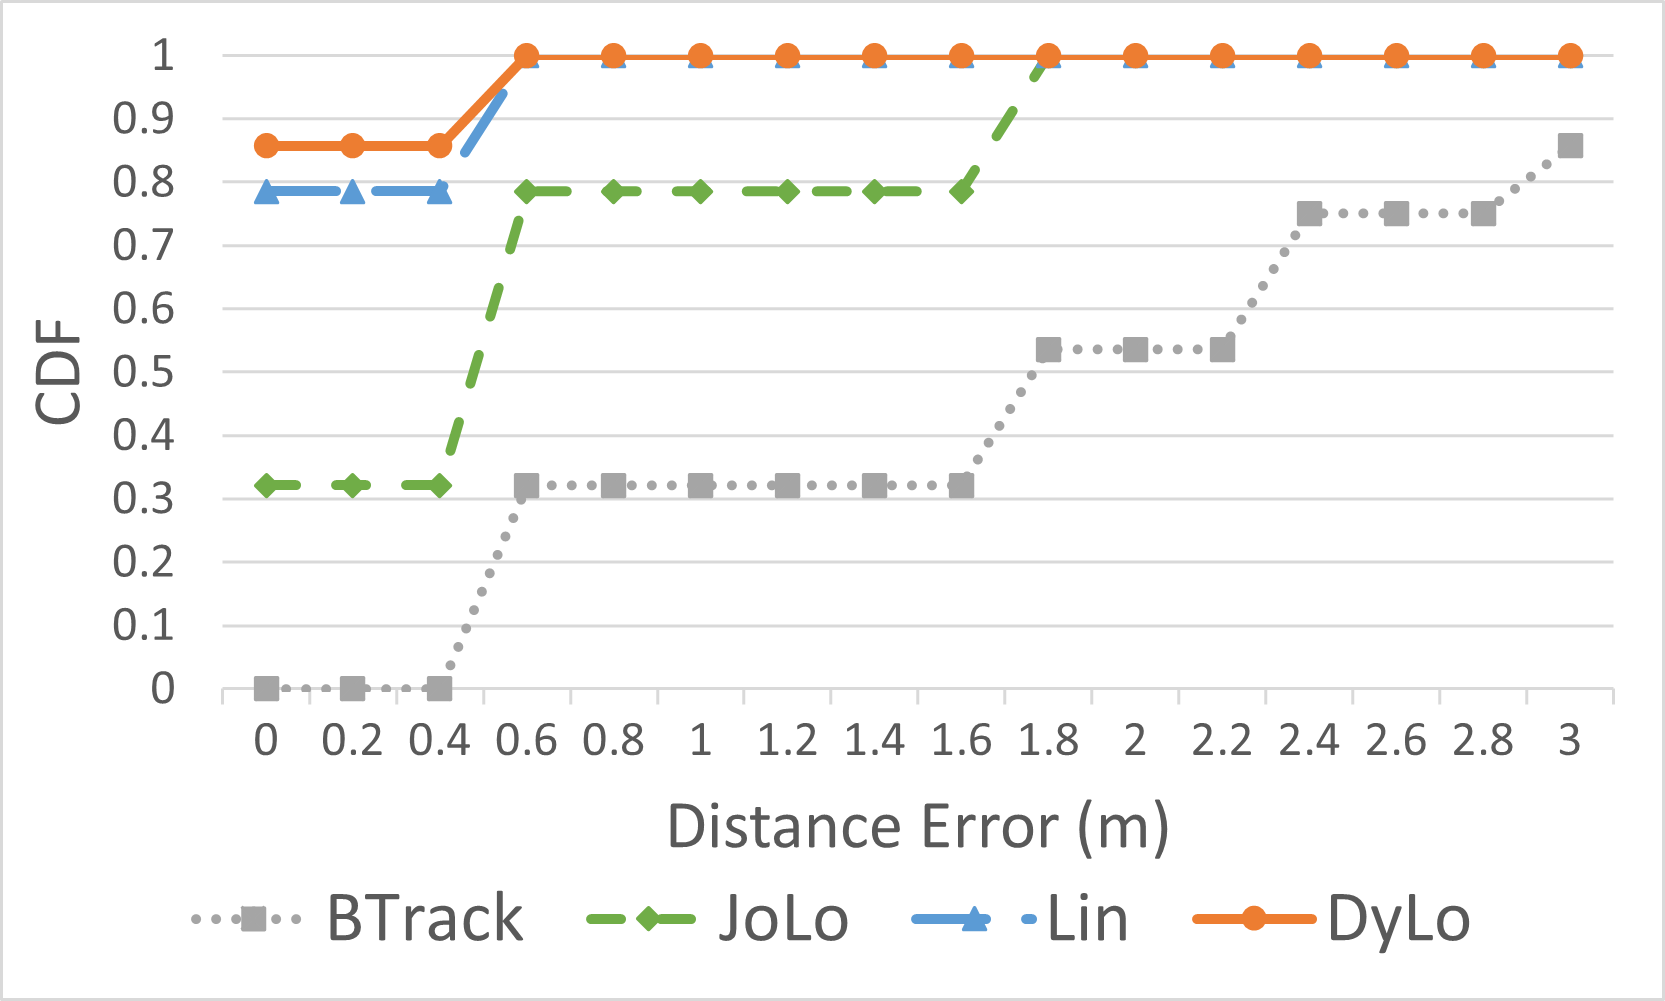
\includegraphics[width=0.72\textwidth]{images/5_1_Comparisons_with_Other_Methods_CDF_ST.png}
        \caption{CDFs of stationary}
        \label{figure:5_1_Comparisons_with_Other_Methods_CDF_ST}
    \end{subfigure}
    %\caption{.}
% subfigs for scripted walk
    % \centering
    \begin{subfigure}{1\linewidth}
    \centering
        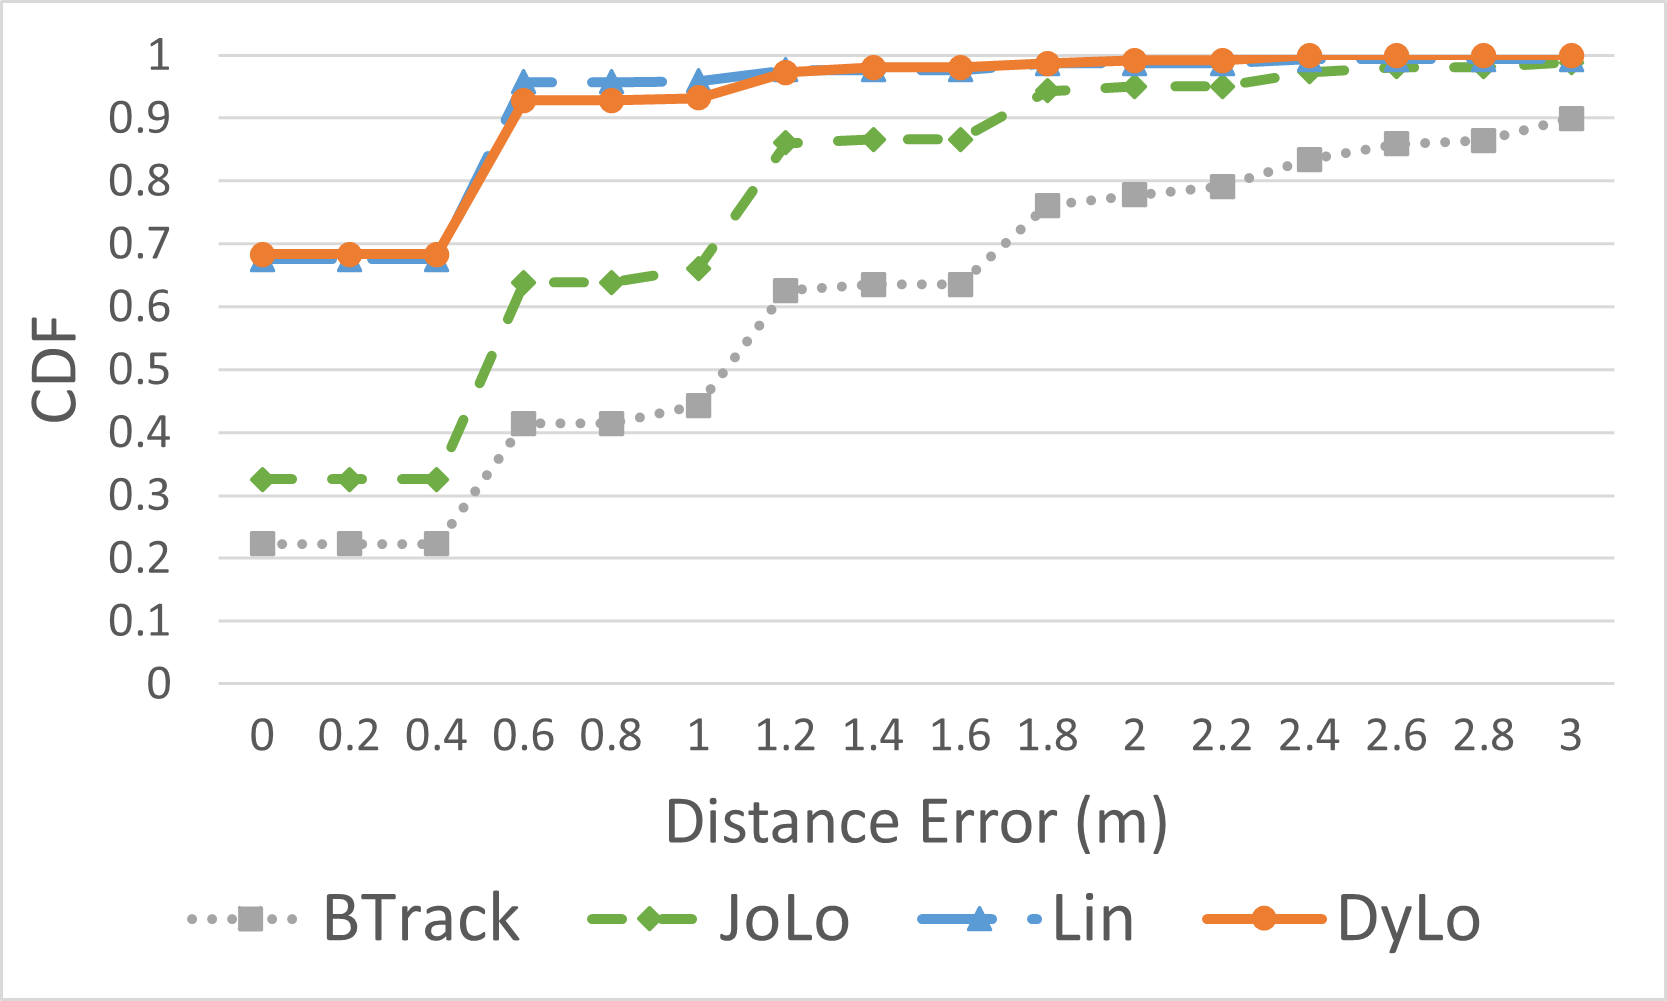
\includegraphics[width=0.72\textwidth]{images/5_1_Comparisons_with_Other_Methods_CDF_SW.png}
        \caption{CDFs of scripted walk}
        \label{figure:5_1_Comparisons_with_Other_Methods_CDF_SW}
    \end{subfigure}
    %\caption{.}
% subfigs for free walk
    % \centering
    \begin{subfigure}{1\linewidth}
    \centering
        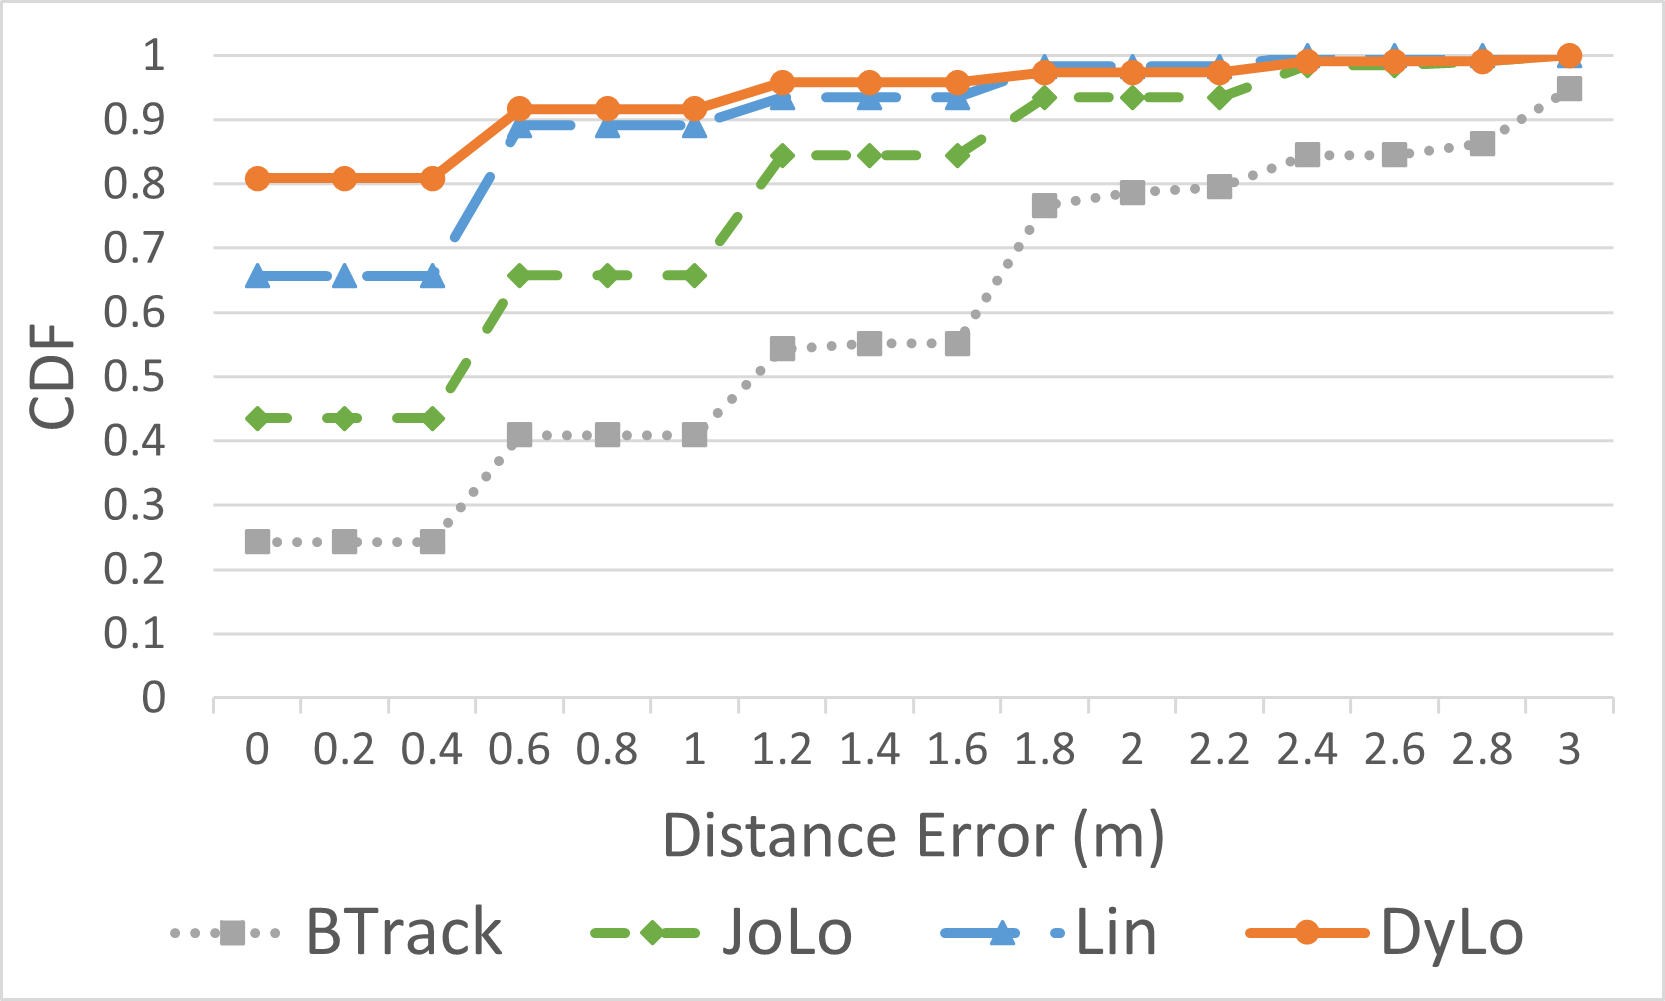
\includegraphics[width=0.72\textwidth]{images/5_1_Comparisons_with_Other_Methods_CDF_FW.png}
        \caption{CDFs of free walk}
        \label{figure:5_1_Comparisons_with_Other_Methods_CDF_FW}
    \end{subfigure}
\caption{Cumulative distribution functions of each scenario.}
\label{figure:5_1_Comparisons_with_Other_Methods_CDF}
\end{figure}
%=== figure === %

%paragraph 
\paragraph{}
Their detailed mean distance error (MDE) , standard deviation of the distance error (SDE) and percentiles are shown in Table~\ref{table:5_1_MDEs_and_Percentiles_ST}, Table~\ref{table:5_1_MDEs_and_Percentiles_SW}, and Table~\ref{table:5_1_MDEs_and_Percentiles_FW}. Through the experiment results of each scenario, We can find that because of the design of wireless filter and dynamic weighting, the positioning performance of $DyLo$ is better than the other three existing methods, especially in the irregular free walk scenario.

% === table === %
\begin{table}
    \begin{center}
    \caption{MDEs and percentiles of proposed methods and baselines of stationary}
    \label{table:5_1_MDEs_and_Percentiles_ST}
        \begin{tabular}{|c||c|c|c|c|}
            \hline
                Method & MDE & SDE & 70\% Percentile & 90\% Percentile \\
            \hline
            \hline
                $BTrack$ & 1.85 m  & 0.92 m  & 2.35 m & 3.06 m \\
            \hline
                $JoLo$   & 0.66 m  & 0.42 m  & 0.56 m & 1.71 m \\
            \hline
                $Lin$    & 0.129 m & 0.061 m & 0 m    & 0.51 m \\
            \hline
                $DyLo$   & 0.086 m & 0.053 m & 0 m    & 0.46 m \\
            \hline
        \end{tabular}
    \end{center}
\end{table}
% === table === %

% === table === %
\begin{table}
    \begin{center}
    \caption{MDEs and percentiles of proposed methods and baselines of scripted walk}
    \label{table:5_1_MDEs_and_Percentiles_SW}
        \begin{tabular}{|c||c|c|c|c|}
            \hline
                Method & MDE & SDE & 70\% Percentile & 90\% Percentile \\
            \hline
            \hline
                $BTrack$ & 1.35 m  & 1.35 m & 1.7 m  & 3 m \\
            \hline
                $JoLo$   & 0.75 m  & 0.6 m  & 1.04 m & 1.69 m \\
            \hline
                $Lin$    & 0.254 m & 0.25 m & 0.42 m & 0.56 m \\
            \hline
                $DyLo$   & 0.249 m & 0.18 m & 0.41 m & 0.58 m \\
            \hline
        \end{tabular}
    \end{center}
\end{table}
% === table === %

% === table === %
\begin{table}
    \begin{center}
    \caption{MDEs and percentiles of proposed methods and baselines of free walk}
    \label{table:5_1_MDEs_and_Percentiles_FW}
        \begin{tabular}{|c||c|c|c|c|}
            \hline
                Method & MDE & SDE & 70\% Percentile & 90\% Percentile \\
            \hline
            \hline
                $BTrack$ & 1.35 m & 1.31 m & 1.74 m & 2.89 m \\
            \hline
                $JoLo$   & 0.69 m & 0.59 m & 1.05 m & 1.72 m \\
            \hline
                $Lin$    & 0.32 m & 0.31 m & 0.44 m & 1 m \\
            \hline
                $DyLo$   & 0.21 m & 0.29 m & 0 m    & 0.57 m \\
            \hline
        \end{tabular}
    \end{center}
\end{table}
% === table === %


%*----------------------section 5.2
\section{Contribution Between Wireless and Image}
\paragraph{}
This section explores the respective contributions of wireless and image to the Dynamic Localization System. The system uses the wireless signal and image data separately to locate, then calculates the MDE and SDE to evaluate the performance. Since the image phase uses the positioning results of the wireless phase for wireless filtering to limit the size of the image database, the image will evaluate the performance of wireless filtering. Their detailed MDEs and SDEs are shown in Table~\ref{table:5_2_MDEs_and_SDEs_between_wireless_and_image_of_Dynamic_Localization_System}. $Image$ means the results of only image phase; $Wireless$ means the results of only wireless phase; $Image$ $with$ $WF$ means the results of image phase using wireless filtering.

\paragraph{}
$Image$ has a gap with $Wireless$ whether in MDE or SDE. First of all, because the wireless data is optimized by data preprocessing and enhancing, it performs exceptionally well. Another reason is that when positioning in image phase, it will be misled by similar image features in the environment, resulting in huge errors in image positioning. However, when we add wireless filtering to the image phase to filter out the positioning errors of the large-scale environment, the $Image$ $with$ $WF$ can achieve high-precision positioning in the small-scale range.

\paragraph{}
In the large-scale environment without wireless filtering, the performance of $Image$ is lost to $Wireless$. However, when wireless filtering is added to limit the scope of small-scale, the performance of $Image$ $with$ $WF$ is better than that of $Wireless$. The contribution of wireless signal is to reduce the large-scale environment to a small-scale range, and the contribution of image data is to complete the most accurate positioning in the small-scale range. Finally, dynamic weighting dynamically adjusts the contribution ratio of wireless and image with the changing environment.

% === table === %
\begin{table}
    \begin{center}
    \caption{MDEs and SDEs between wireless and image of Dynamic Localization System}
    \label{table:5_2_MDEs_and_SDEs_between_wireless_and_image_of_Dynamic_Localization_System}
        \begin{tabular}{|c||c|c||c|c|}
            \hline
                & \multicolumn{2}{|c|}{Scripted Walk} & \multicolumn{2}{|c|}{Free Walk} \\
            \hline
                Method & MDE & SDE & MDE & SDE \\
            \hline
            \hline
                $Image$    & 1.03 m  & 3.03 m & 0.99 m & 2.9 m \\
            \hline
                $Wireless$ & 0.49 m  & 0.28 m & 0.34 m & 0.31 m \\
            \hline
                $Image$ $with$ $WF$ & 0.32 m & 0.21 m & 0.24 m & 0.3 m \\
            \hline
                $DyLo$   & 0.249 m & 0.18 m & 0.21 m & 0.29 m \\
            \hline
        \end{tabular}
    \end{center}
\end{table}
% === table === %

%*----------------------section 5.3
\section{Improvement of Data Enhancing}
\paragraph{}
To discuss the improvement of data enhancing to wireless signal, this section will compare $DyLo$ with $BTrack$ and $JoLo$, and in order to exclude the influence of image data on indoor localization, $DyLo$ will discard image data and simply use wireless signals.
%

%paragraph 
\paragraph{}
As can be seen from Fig.~\ref{figure:5_3_Data_Enhancing_MDE_4}, whether in scripted walk or free walk, the MDE of $JoLo$ and $DyLo$ with multiple devices is better than that of $BTrack$ with a single device. In the comparison of multiple devices, because $DyLo$ uses data enhancing technology, it has more than 50\% improvement compared to $JoLo$ with the same number of devices.
%

%paragraph 
\paragraph{}
And to compare with single-device $BTrack$, we restrict both $JoLo$ and $DyLo$ to be used in single-device situations. In Fig.~\ref{figure:5_3_Data_Enhancing_MDE_1}, the MDE of $BTrack$ and $JoLo$ is similar, and because $DyLo$ uses data enhancing, even with a single mobile phone, the MDE of both free walk and Scripted Walk is at least 23\% better than $BTrack$ and $JoLo$.
%

%paragraph 
\paragraph{}
From the above evaluation of the data enhancing effect to $DyLo$, $DyLo$ with data enhancing outperforms $BTrack$ and $JoLo$ by 50\% and 23\% in multiple devices and single device respectively, so we can infer the improvement of data enhancing to wireless signal is significant.
%

%=== figure 5_3_Data_Enhancing_MDE_4=== %
% subfigs for 4 devices
\begin{figure}[tbph]%\ContinuedFloat
    %\centering
    \begin{subfigure}{1\linewidth}
    \centering
        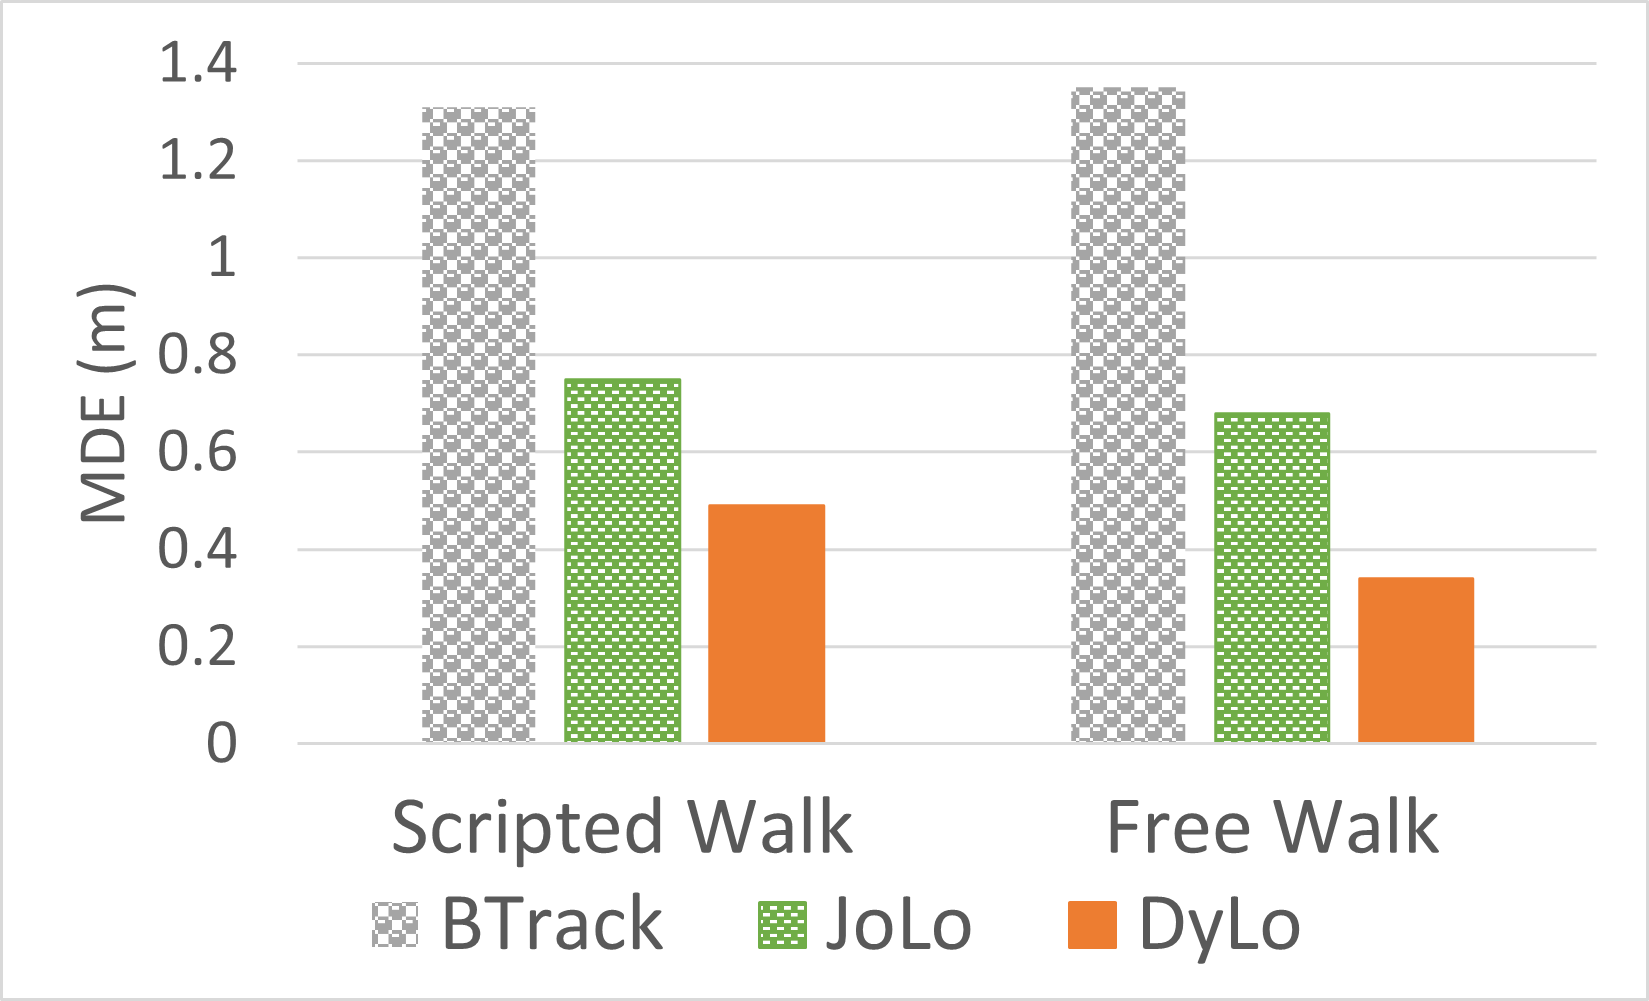
\includegraphics[width=0.8\textwidth]{images/5_3_Data_Enhancing_MDE_4.png}
        \caption{MDEs of improvement in 4 devices}
        \label{figure:5_3_Data_Enhancing_MDE_4}
    \end{subfigure}
    %\caption{.}
% subfigs for 1 device
    % \centering
    \begin{subfigure}{1\linewidth}
    \centering
        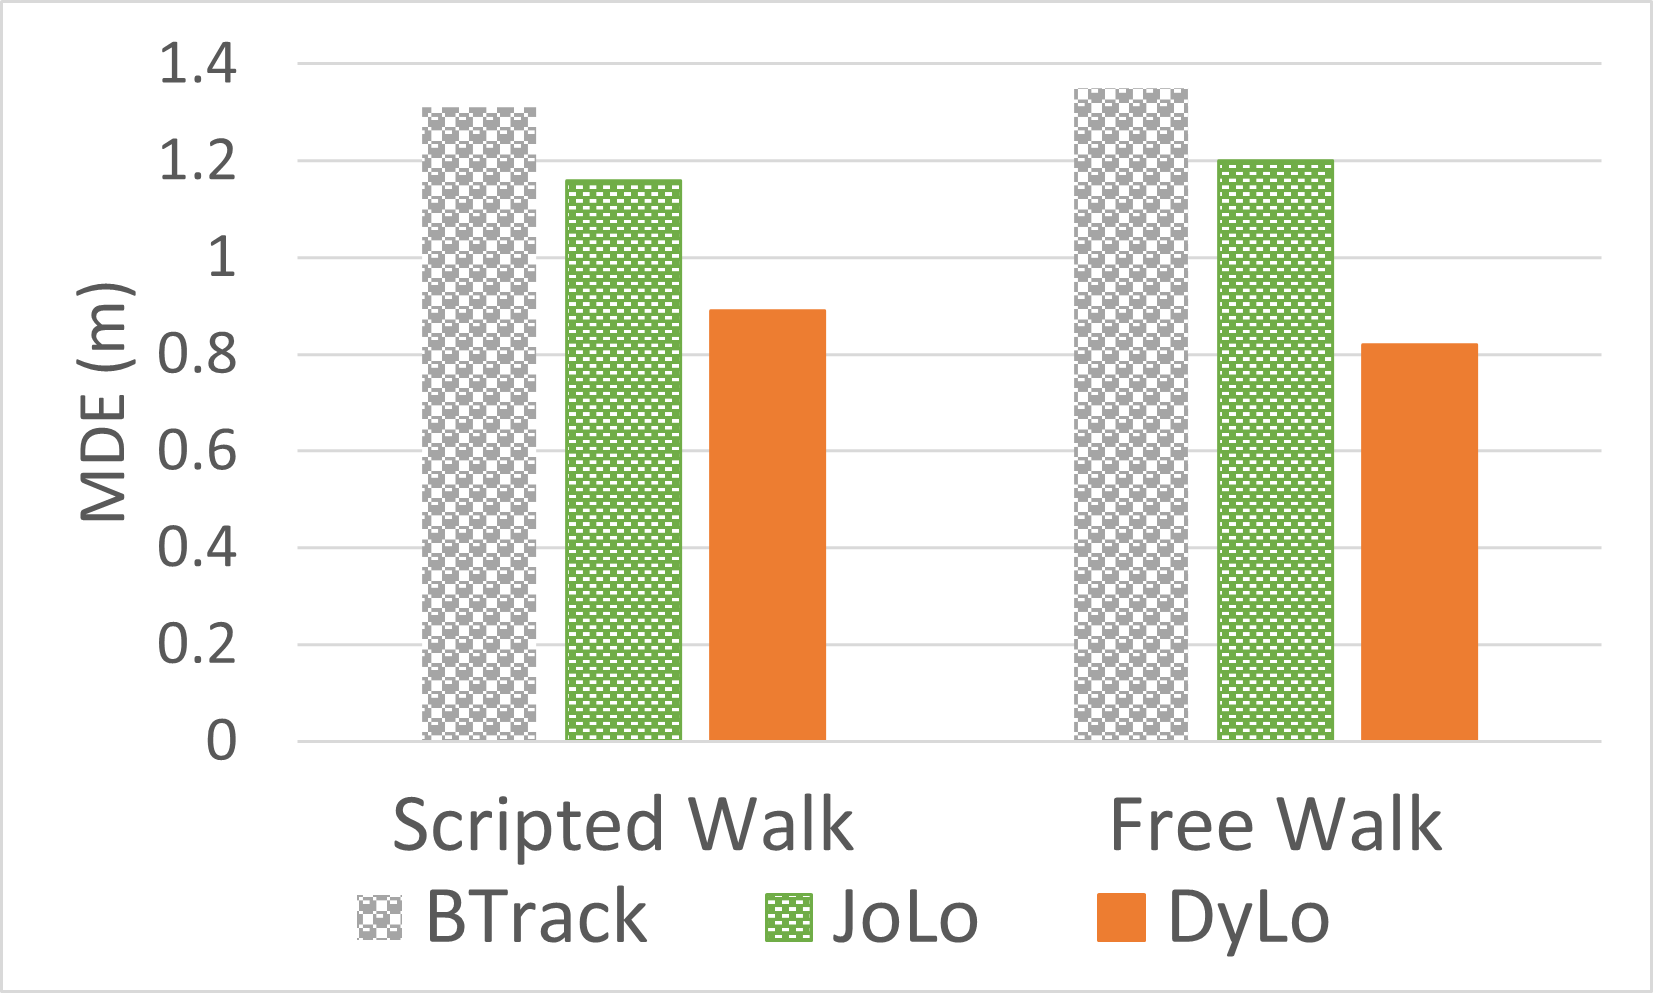
\includegraphics[width=0.8\textwidth]{images/5_3_Data_Enhancing_MDE_1.png}
        \caption{MDEs of improvement in 1 device}
        \label{figure:5_3_Data_Enhancing_MDE_1}
    \end{subfigure}
\caption{MDEs of each number of devices with improvement of data enhancing.}
\label{figure:5_3_Data_Enhancing_MDE}
\end{figure}
%=== figure === %


%*----------------------section 5.4
\section{Effects of Different Environments}

\subsection{Setup}
%paragraph
\paragraph{}
To verify that our method is not limited to our office environment, the system is effective in different-sized environments. In this section, we find another office environment Room 92508, also located in the Electrical Engineering (EE) Department of National Cheng Kung University (NCKU), Tainan, Taiwan, for evaluation shown in Fig.~\ref{figure:5_4_Different_Environments_picture}.
%

%paragraph
\paragraph{}
As the plan of Room 92508 is shown in Fig.~\ref{figure:5_4_Different_Environments_plan}, Room 92508 is a smaller rectangular office than Room 92589. There is a partition in the middle of the office to separate the office into two areas. We plan 34 positioning points in the remaining aisle space. The positioning point is a square grid of 0.6m * 0.6m, forming an experimental area with a length of 6.6 meters and a width of 4.2 meters, and deploys 6 wireless beacons around the environment with 1.7 meters above the ground. The environmental differences between the two are shown in Table. The experimental scenarios are the same as Room 92589, with scripted walk and free walk respectively evaluating two scenarios with regularity and irregularity.
%

%=== figure 5_4_Different_Environments_picture=== %
% subfigs for Office environment
\begin{figure}[tbph]%\ContinuedFloat
    %\centering
    \begin{subfigure}{1\linewidth}
    \centering
        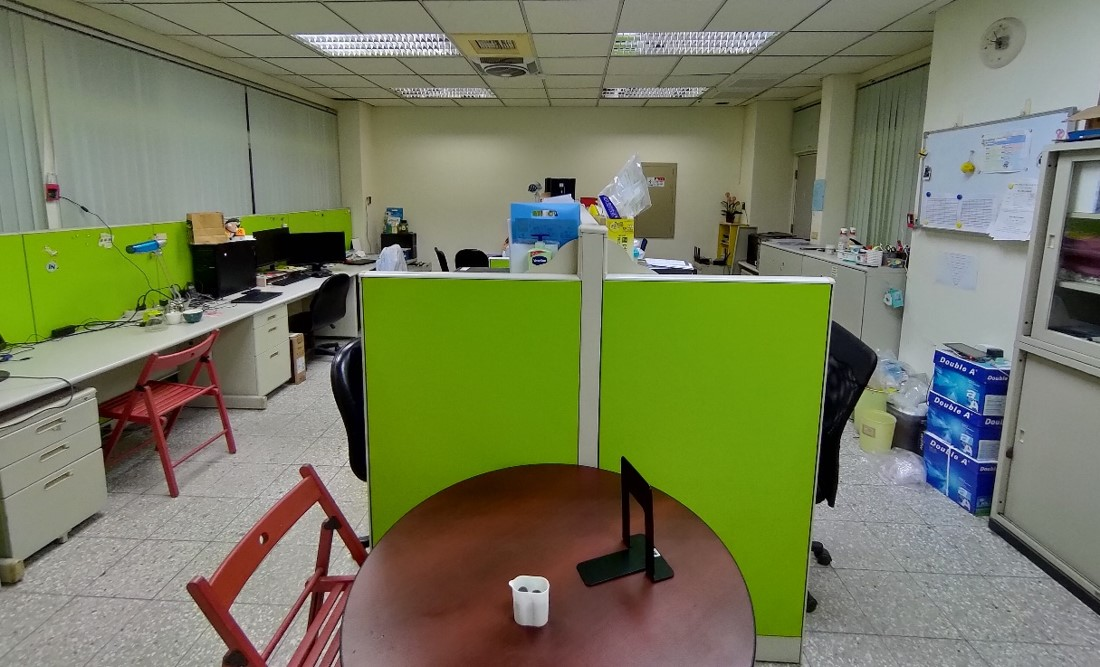
\includegraphics[width=0.8\textwidth]{images/5_4_Different_Environments_picture.jpg}
        \caption{Office environment of room 92508}
        \label{figure:5_4_Different_Environments_picture}
    \end{subfigure}
    %\caption{.}
% subfigs for Room plan
    % \centering
    \begin{subfigure}{1\linewidth}
    \centering
        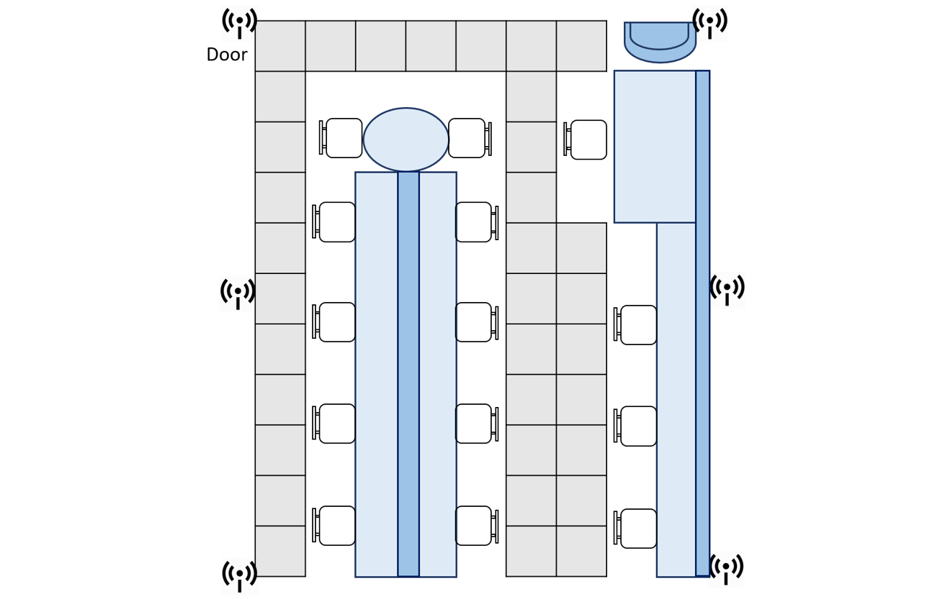
\includegraphics[width=0.85\textwidth]{images/5_4_Different_Environments_plan.png}
        \caption{Room plan of 92508}
        \label{figure:5_4_Different_Environments_plan}
    \end{subfigure}
\caption{Environment and room plan of room 92508.}
\label{figure:5_4_Different_Environments}
\end{figure}
%=== figure === %

\subsection{Results}
%paragraph
\paragraph{}
The experimental results are shown in Fig.~\ref{figure:5_4_Different_Environment_MDE}. The performance of $DyLo$ does not vary due to changes in the environment, and still performs well due to the excellent dynamic adjustment between wireless and image. In particular, as shown in Fig.~\ref{figure:5_4_Different_Environment_MDE_FW}, in the irregular scenario as free walk, $DyLo$ outperforms the other three methods due to the excellent system design of dynamic adjustment. Therefore, $DyLo$ benefits from its excellent system design, and excellent dynamic adjustment between wireless and image, making it still perform well in different environments.
%

%=== figure 5_4_Different_Environment_MDE=== %
% subfigs for scripted walk
\begin{figure}[tbph]%\ContinuedFloat
    %\centering
    \begin{subfigure}{1\linewidth}
    \centering
        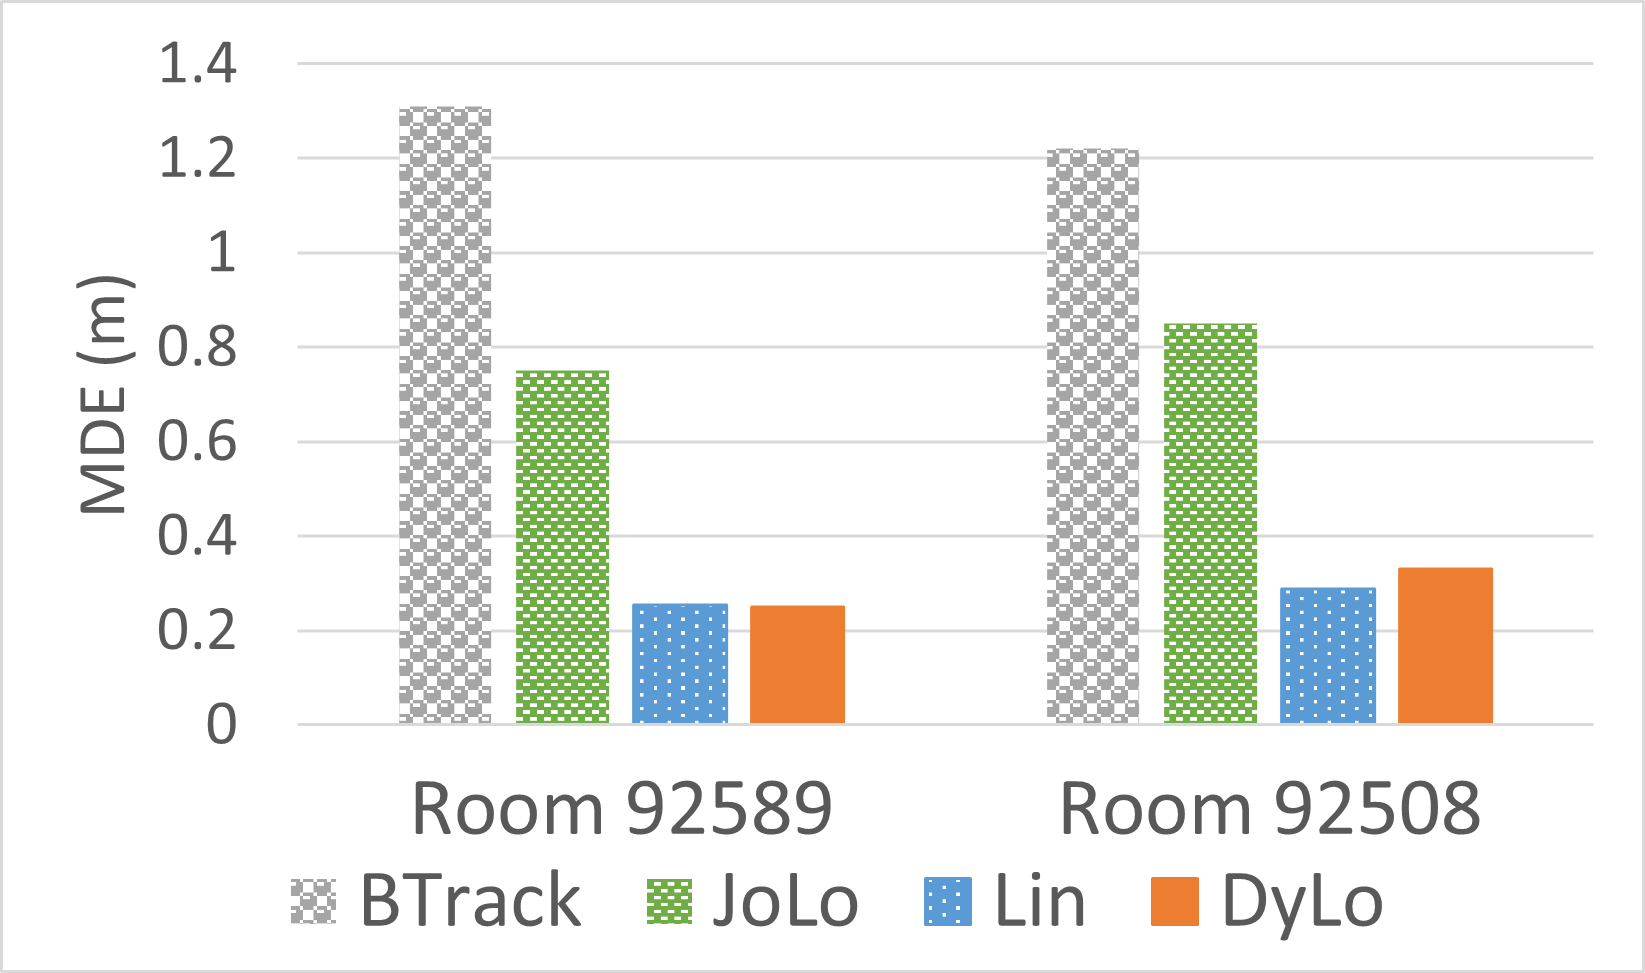
\includegraphics[width=0.8\textwidth]{images/5_4_Different_Environment_MDE_SW.png}
        \caption{MDEs of scripted walk}
        \label{figure:5_4_Different_Environment_MDE_SW}
    \end{subfigure}
    %\caption{.}
% subfigs for free walk
    % \centering
    \begin{subfigure}{1\linewidth}
    \centering
        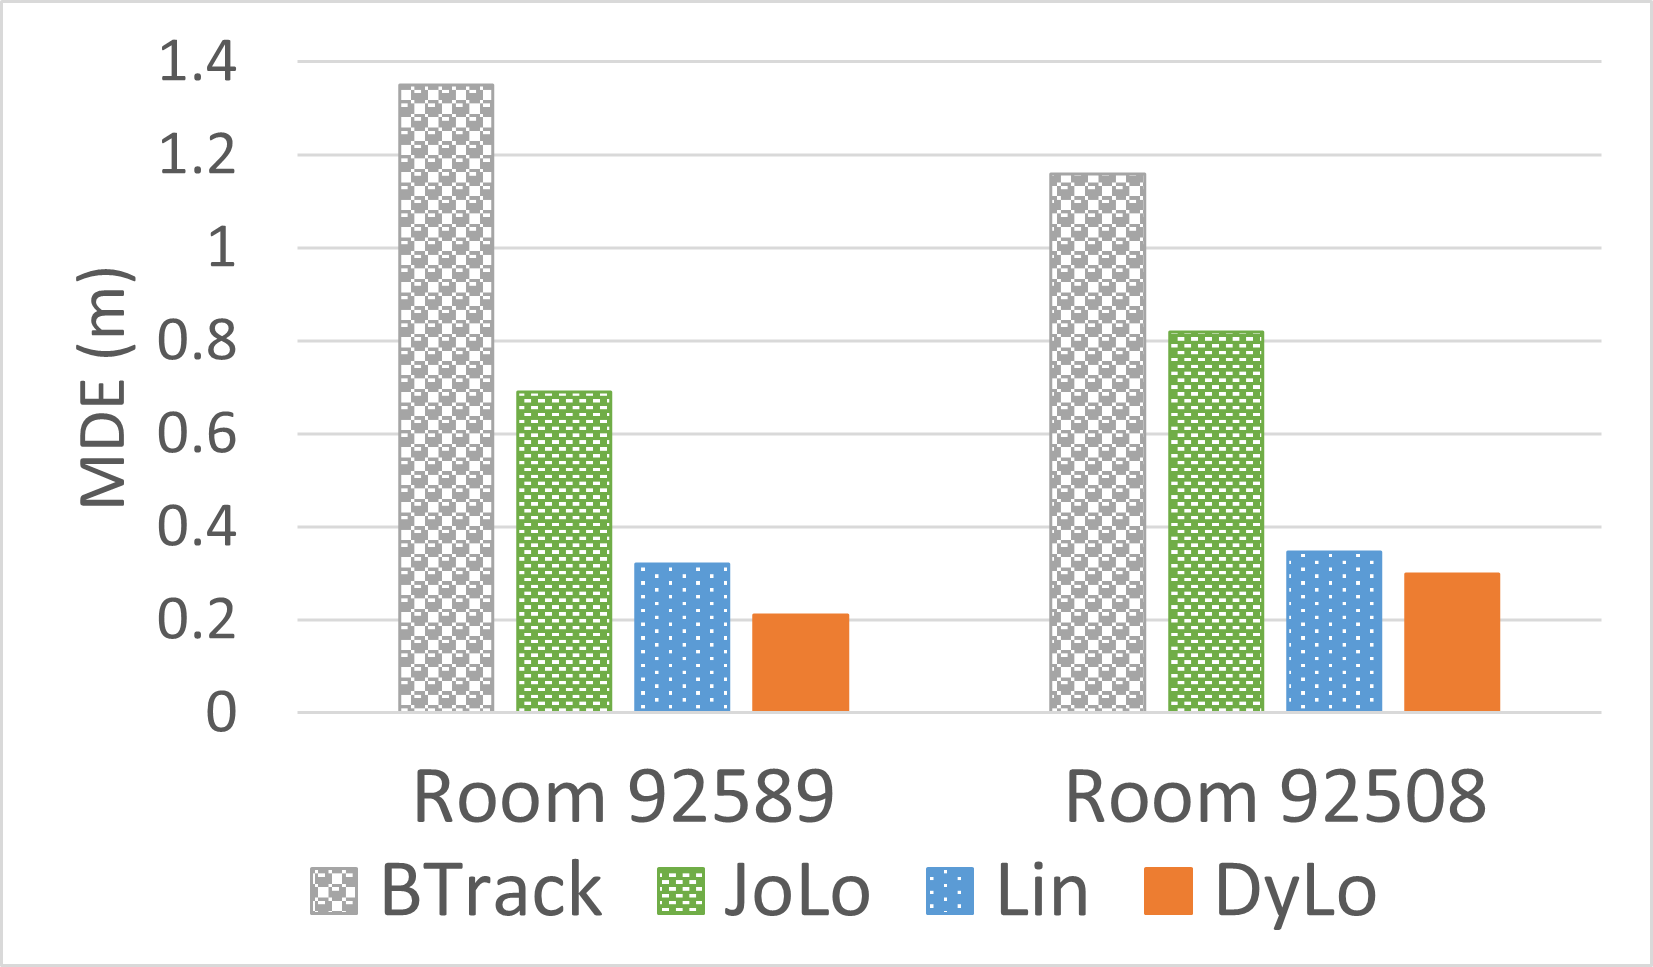
\includegraphics[width=0.8\textwidth]{images/5_4_Different_Environment_MDE_FW.png}
        \caption{MDEs of free walk}
        \label{figure:5_4_Different_Environment_MDE_FW}
    \end{subfigure}
\caption{MDEs of each scenario with in different environment.}
\label{figure:5_4_Different_Environment_MDE}
\end{figure}
%=== figure === %

%*----------------------section 5.5
\section{Effects of the Number of Wireless Devices and Cameras}
\subsection{Setup}

%paragraph 
\paragraph{}
When the positioning system is actually used, not every four devices are used for positioning, and sometimes only two or even only one devices is used for positioning. Therefore, this section will discuss the impact of different numbers of devices on different positioning systems. We plan the combination of one to four devices as shown in Table~\ref{table:5_5_Device_Combination}, and the combination of different numbers especially corresponds to the camera orientation.

% === table === %
\begin{table}
    \begin{center}
    \caption{Device Combination of the Number of Wireless Devices and Cameras}
    \label{table:5_5_Device_Combination}
        \begin{tabular}{|c|c|}
            \hline
                & Device Combination \\
            \hline
                1 Device  & Samsung A51 \\
            \hline
                2 Devices & Samsung A51 + hTC U11 \\
            \hline
                3 Devices & Samsung A51 + hTC U11 + hTC U19e \\
            \hline
                4 Devices & Samsung A51 + hTC U11 + hTC U19e + Sharp V \\
            \hline
        \end{tabular}
    \end{center}
\end{table}
% === table === %

\subsection{Results}
%paragraph
\paragraph{}
The experimental results are shown in Fig.~\ref{figure:5_5_Number_of_Devices_MDE}. The performance of each system varies due to the number of experimental devices, and the MDE increases as the number of devices decreases. However, it can still be seen that although the positioning error of $DyLo$ increases as the number of devices decreases, key positioning features can be extracted from a small number of devices due to the excellent dynamic adjustment between wireless and image.
%

%paragraph
\paragraph{}
Especially as shown in Fig.~\ref{figure:5_5_Number_of_Devices_MDE_FW}, in the irregular free walk, the performance of $DyLo$ is better than the other three methods due to the excellent system design of dynamic adjustment. Therefore, $DyLo$ benefits from its excellent system design, and excellent dynamic adjustment between wireless and video, so that it still performs well in different numbers of devices.
%

%=== figure 5_5_Number_of_Devices_MDE=== %
% subfigs for scripted walk
\begin{figure}[tbph]%\ContinuedFloat
    %\centering
    \begin{subfigure}{1\linewidth}
    \centering
        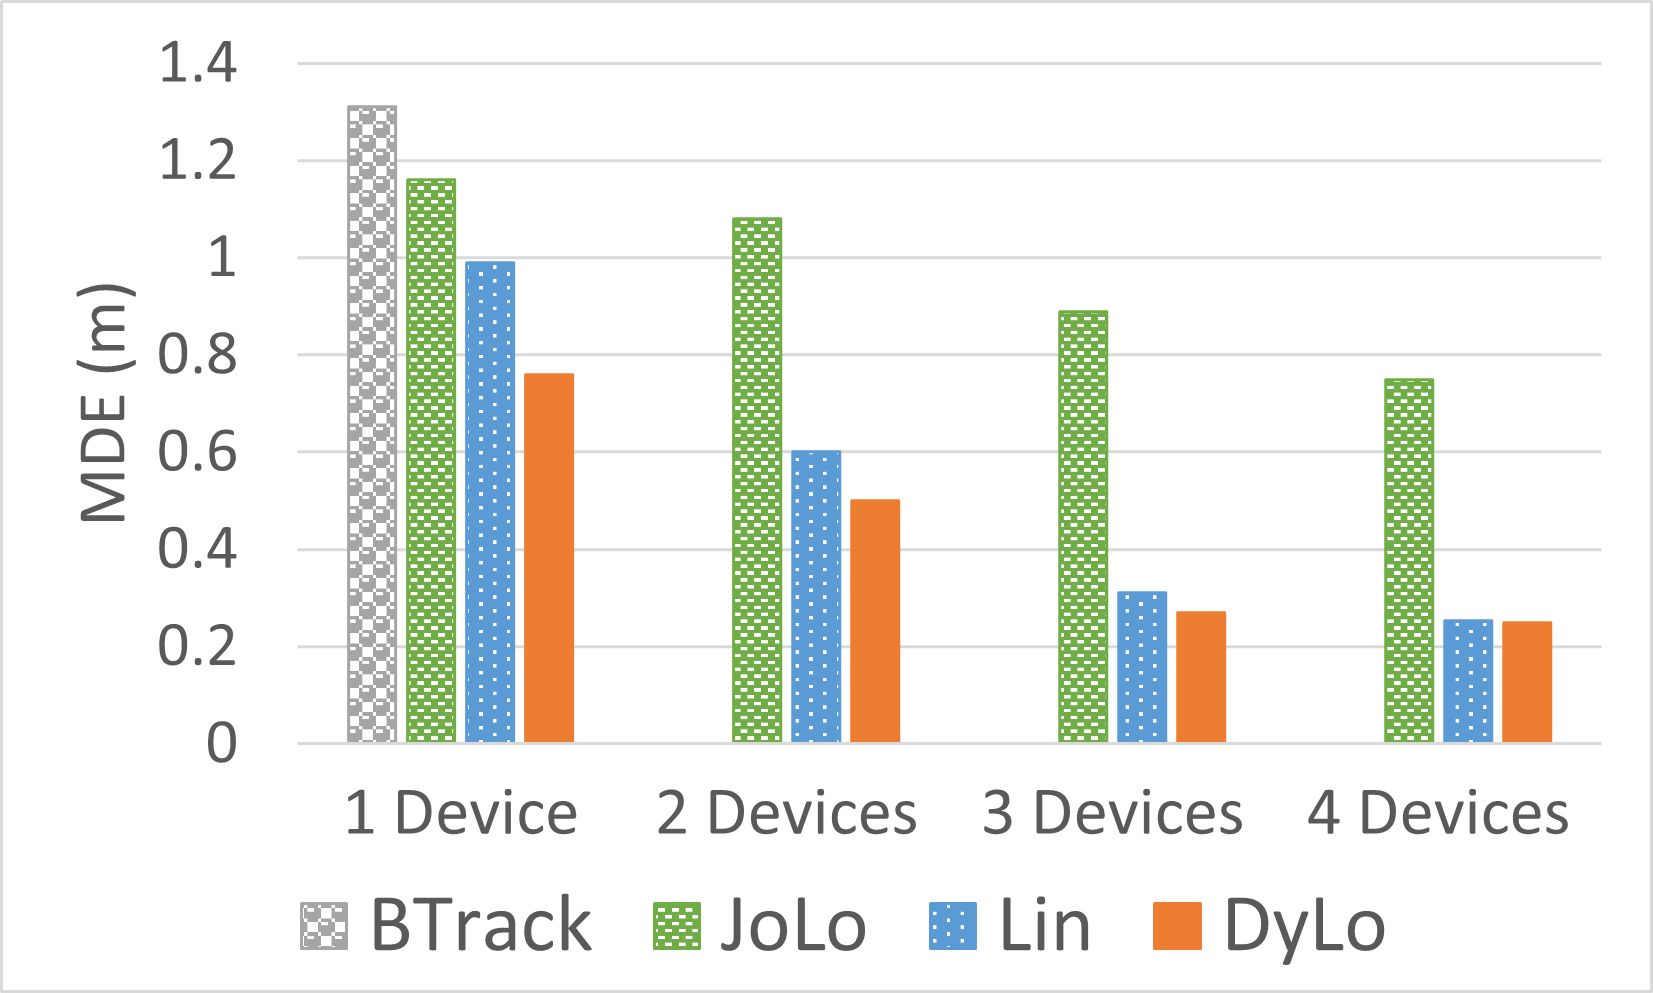
\includegraphics[width=0.8\textwidth]{images/5_5_Number_of_Devices_MDE_SW.png}
        \caption{MDEs of scripted walk}
        \label{figure:5_5_Number_of_Devices_MDE_SW}
    \end{subfigure}
    %\caption{.}
% subfigs for free walk
    % \centering
    \begin{subfigure}{1\linewidth}
    \centering
        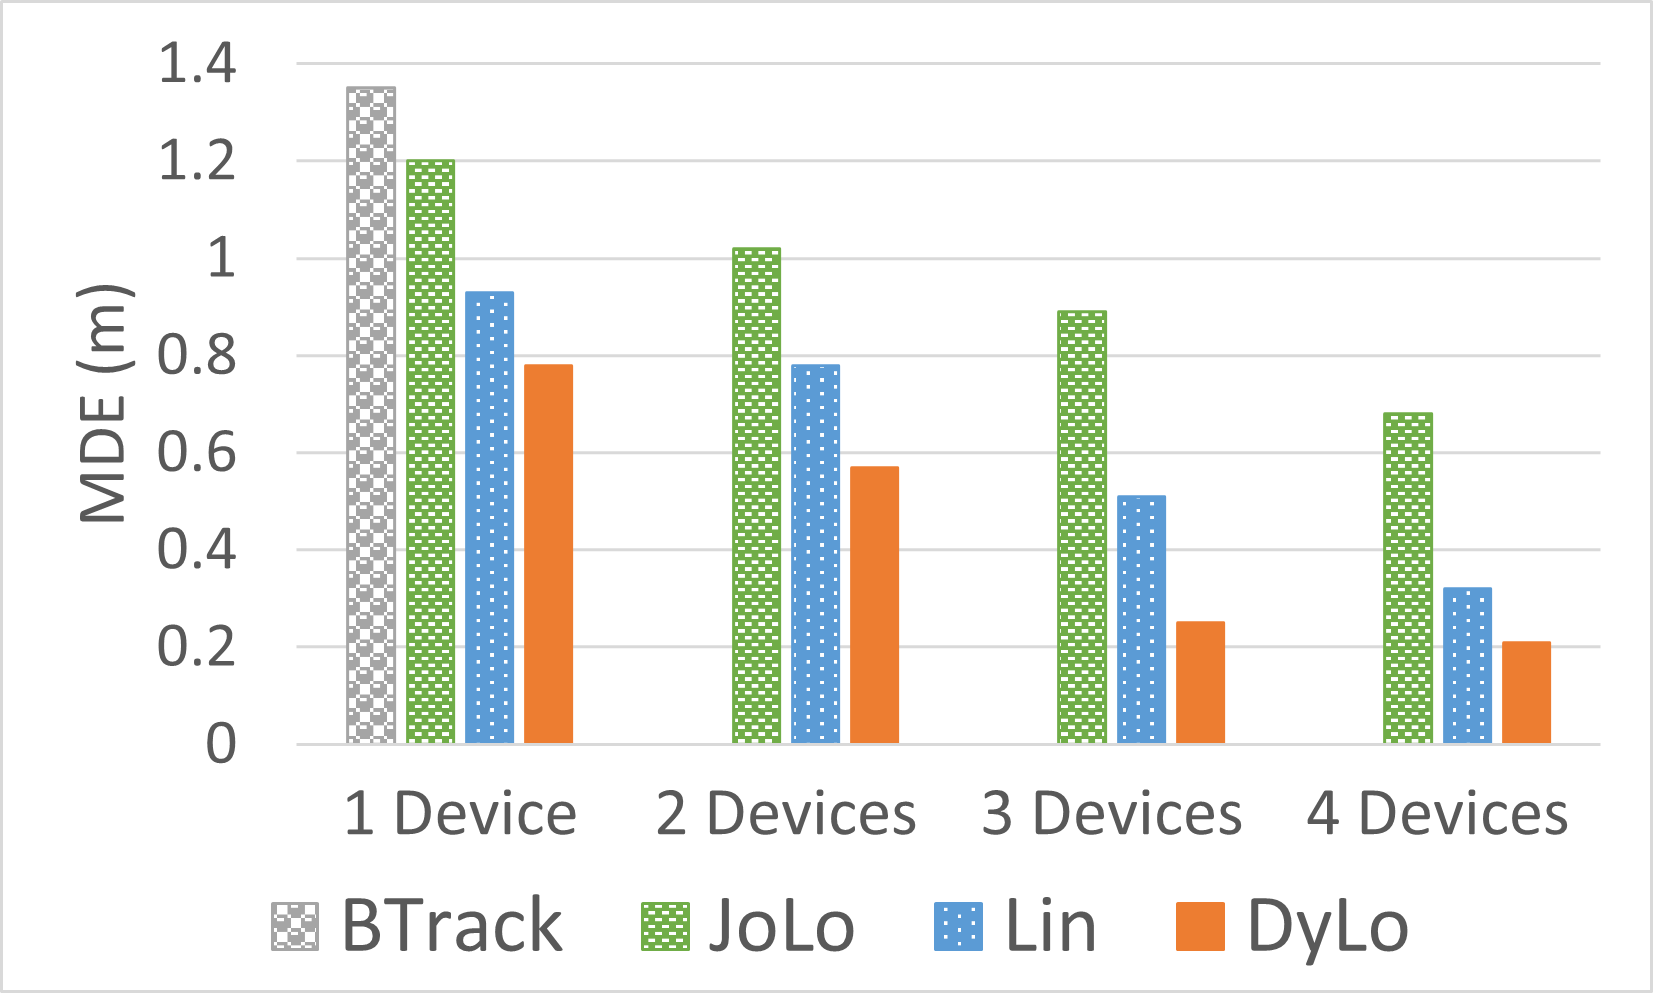
\includegraphics[width=0.8\textwidth]{images/5_5_Number_of_Devices_MDE_FW.png}
        \caption{MDEs of free walk}
        \label{figure:5_5_Number_of_Devices_MDE_FW}
    \end{subfigure}
\caption{MDEs of each scenario with different number of wireless devices and cameras.}
\label{figure:5_5_Number_of_Devices_MDE}
\end{figure}
%=== figure === %

%*----------------------section 5.6
\section{Effects of Blocked Object Problem}
\subsection{Setup}

\paragraph{}
Image hash localization in our system is very dependent on the objects detected in the image. However, objects in real scenes are very susceptible to changes due to human behavior, such as objects being moved or blocked. As shown in Fig.~\ref{figure:5_6_Blocked_Object_Setup_Original}, the original system detected two monitors, one keyboard, and one mouse. However, when the object in the image is blocked as shown in Fig.~\ref{figure:5_6_Blocked_Object_Setup_Blocked}, the detected object will be missing one monitor and one mouse. This section is to discuss the problem of such blocked object.

\paragraph{}
We ignore some detected objects in testing image data randomly to simulate this situation. In the experiment, the parameter $R$ ( 0 <= $R$ <= 1) is used to represent the ratio of objects that are not ignored. For example, $R$=0.6 means that 40\% of the objects are randomly ignored.

%=== figure 5_6_Blocked_Object_Own_MDE=== %
% subfigs for scripted walk
\begin{figure}[tbph]%\ContinuedFloat
    %\centering
    \begin{subfigure}{1\linewidth}
    \centering
        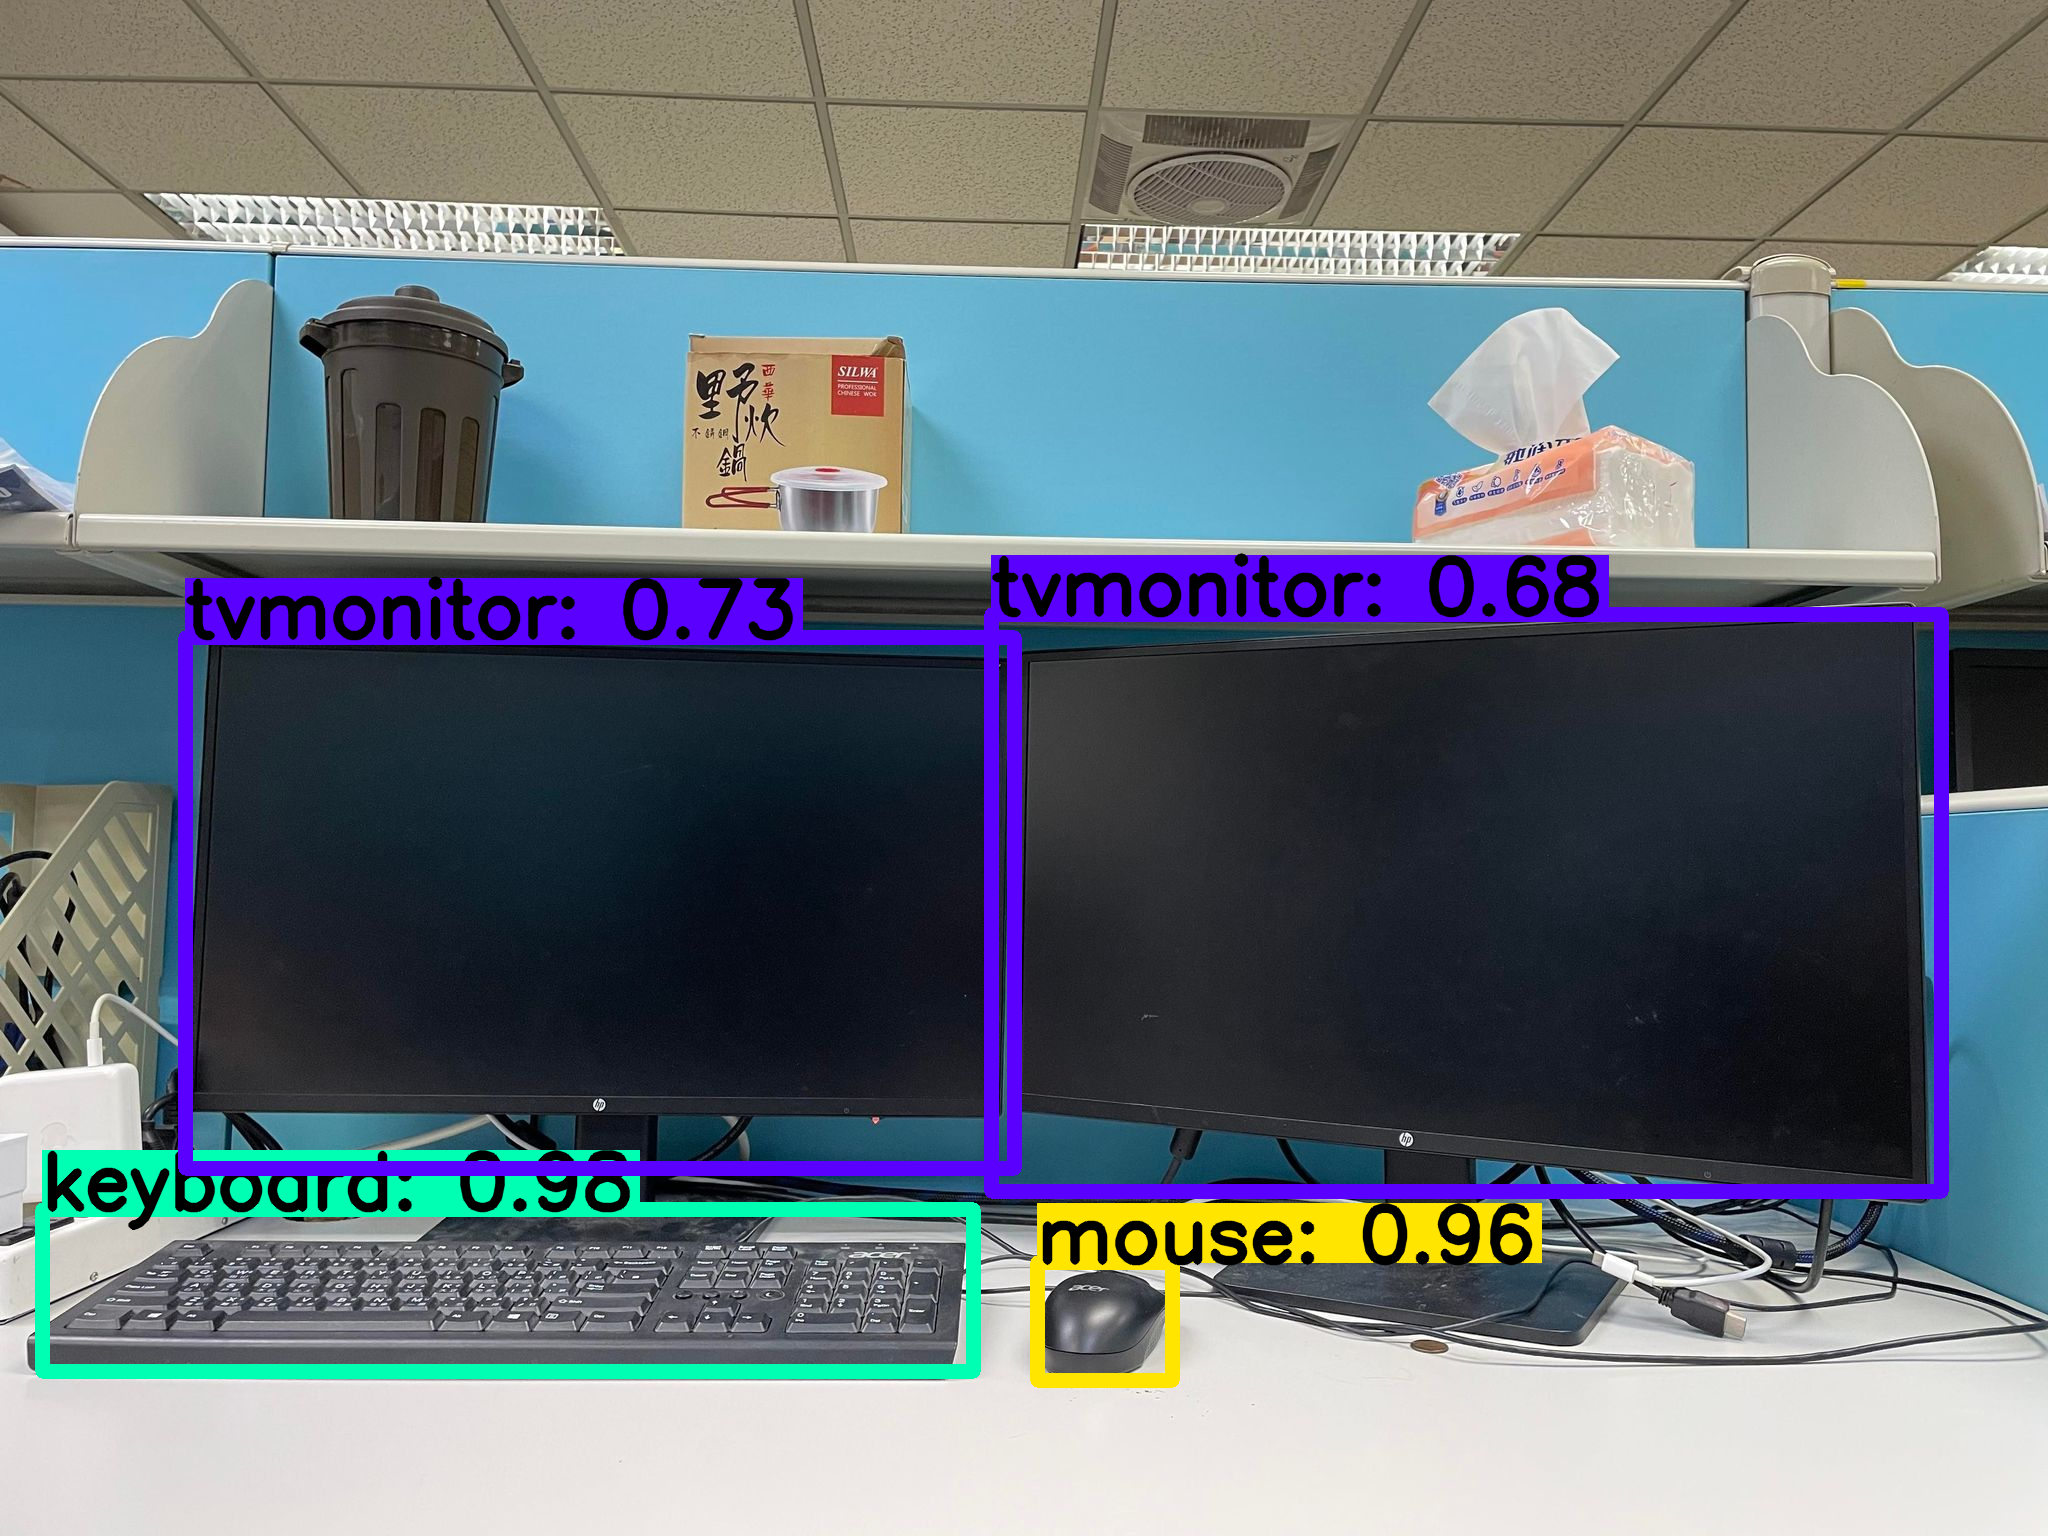
\includegraphics[width=0.8\textwidth]{images/5_6_Blocked_Object_Setup_Original.png}
        \caption{Object without blocked}
        \label{figure:5_6_Blocked_Object_Setup_Original}
    \end{subfigure}
    %\caption{.}
% subfigs for free walk
    % \centering
    \begin{subfigure}{1\linewidth}
    \centering
        \includegraphics[width=0.8\textwidth]{images/5_6_Blocked_Object_Setup_Blocked.png}
        \caption{Object with blocked}
        \label{figure:5_6_Blocked_Object_Setup_Blocked}
    \end{subfigure}
\caption{An example of blocked object.}
\label{figure:5_6_Blocked_Object_Setup}
\end{figure}
%=== figure === %


\subsection{Results}

\paragraph{}
Fig.~\ref{figure:5_6_Blocked_Object_Own_MDE} presents the MDE changes of $DyLo$ facing different degrees of blocked object. Where $I(n)$ represents the $DyLo$ using $n$ cameras and no wireless devices, and $D(m,n)$ represents the $DyLo$ using $m$ wireless devices and $n$ cameras. The MDEs of $I(n)$ increase with the change of $R$ greatly than the MDEs of $D(m,n)$, indicating that the impact of blocked objects on image positioning is huge. When the image cannot detect the object to locate, the image location will become unavailable. The addition of the use of wireless signal in the system will reduce the increase of the positioning error.

%=== figure 5_6_Blocked_Object_Own_MDE=== %
% subfigs for scripted walk
\begin{figure}[tbph]%\ContinuedFloat
    %\centering
    \begin{subfigure}{1\linewidth}
    \centering
        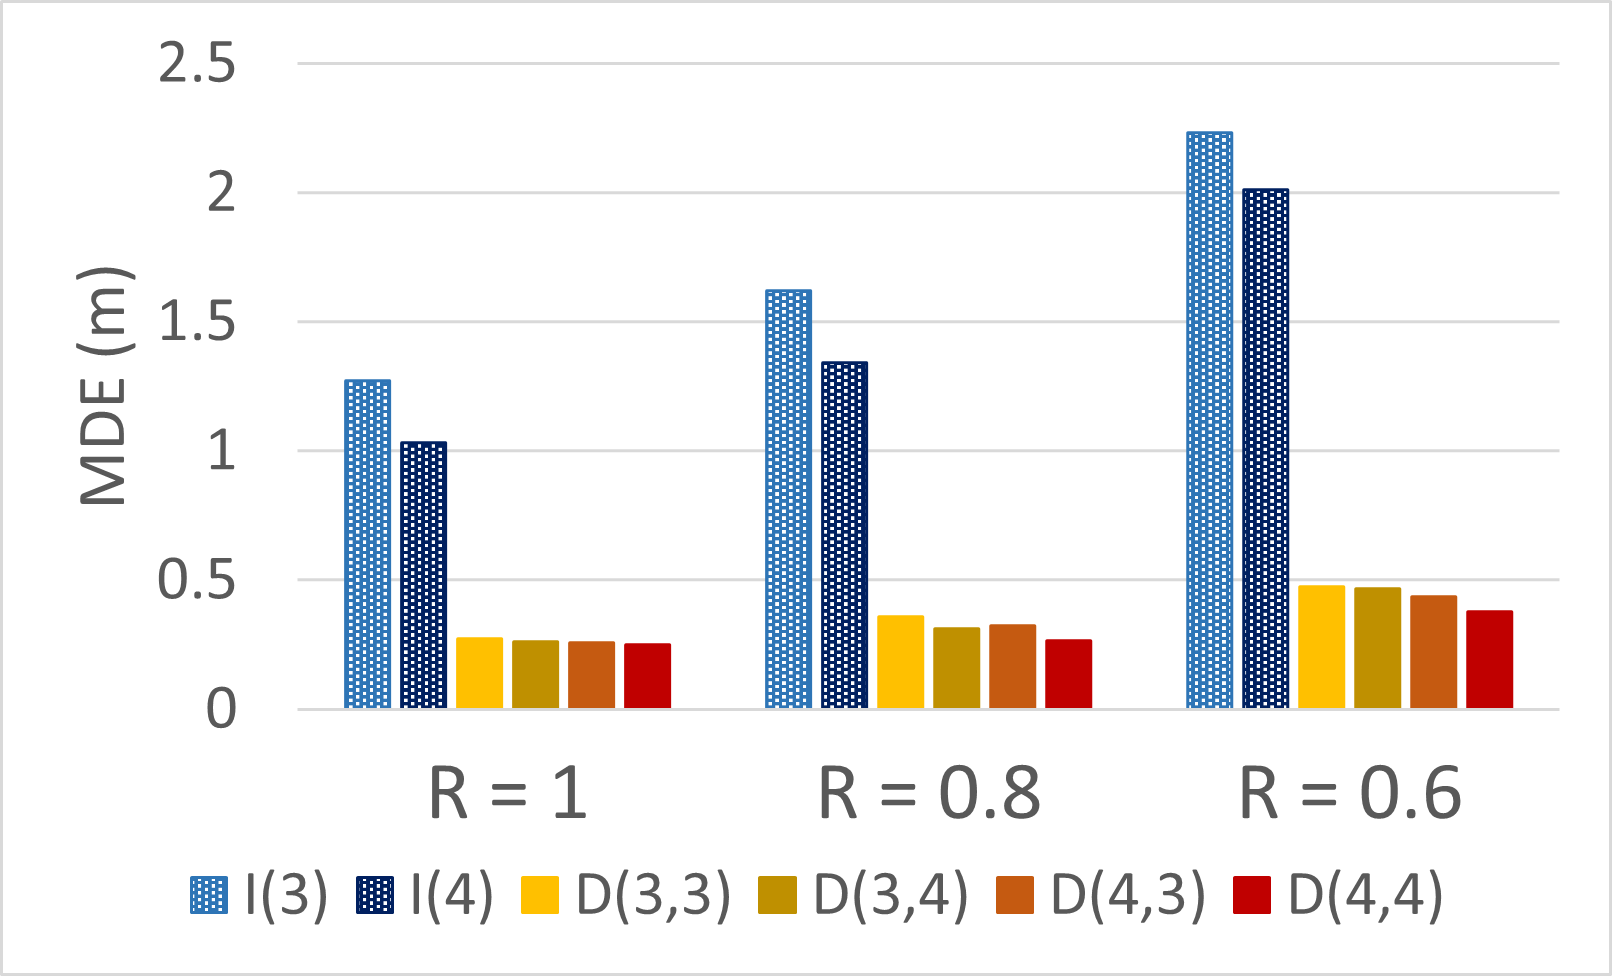
\includegraphics[width=0.8\textwidth]{images/5_6_Blocked_Object_Own_MDE_SW.png}
        \caption{MDEs of scripted walk}
        \label{figure:5_6_Blocked_Object_Own_MDE_SW}
    \end{subfigure}
    %\caption{.}
% subfigs for free walk
    % \centering
    \begin{subfigure}{1\linewidth}
    \centering
        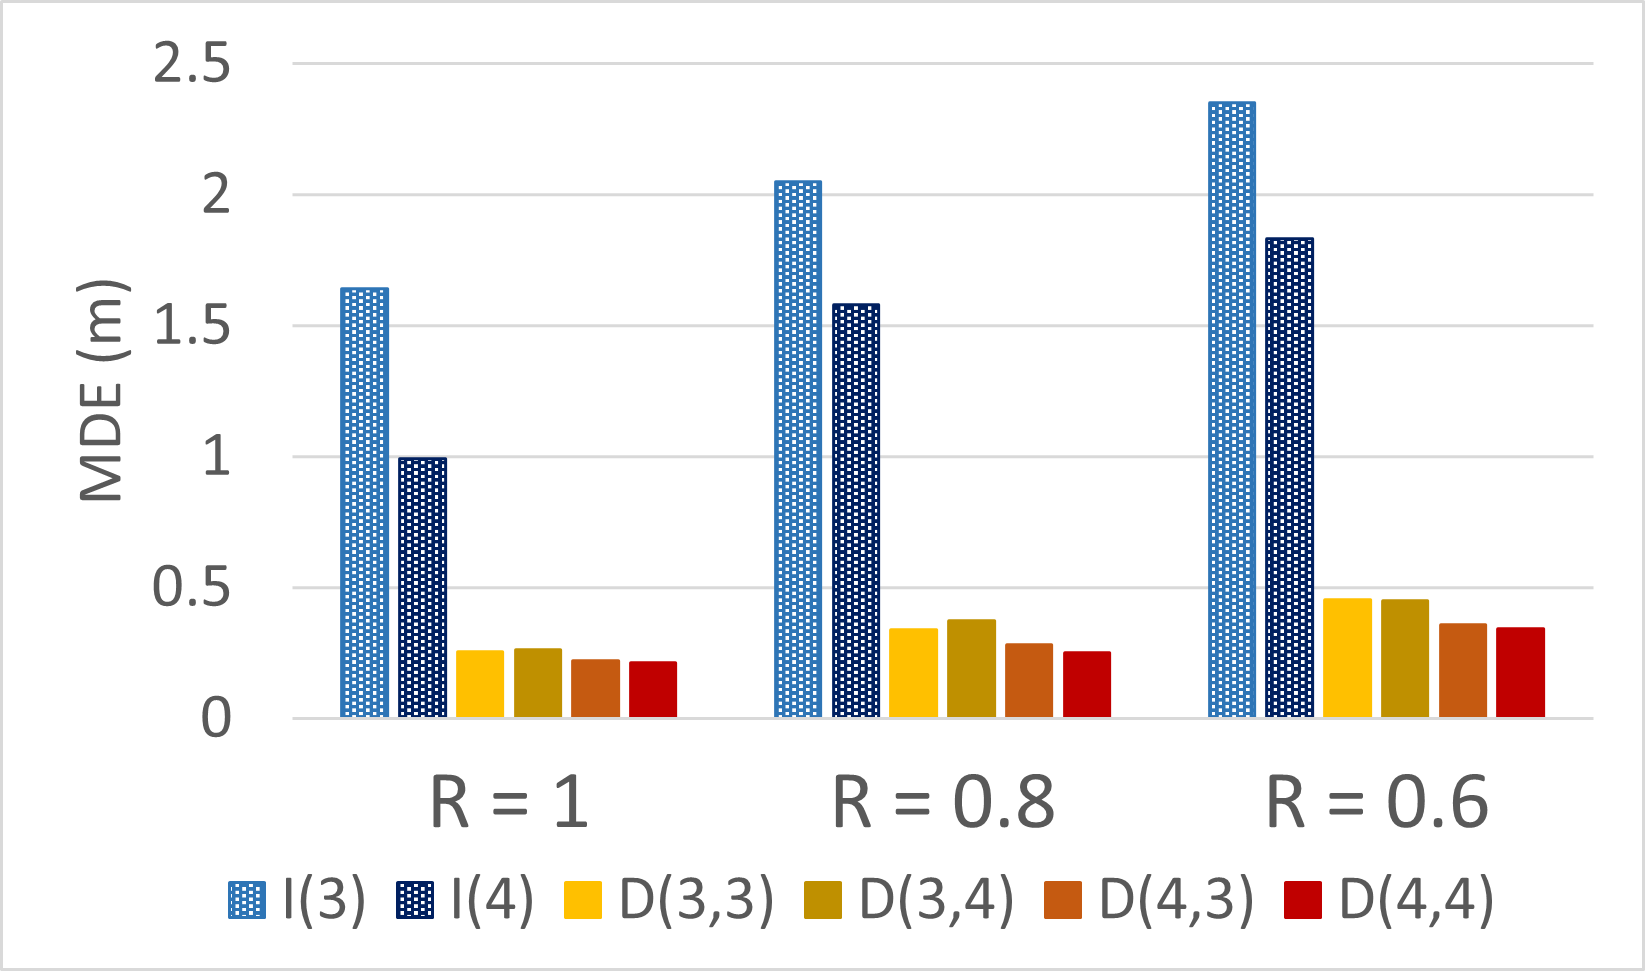
\includegraphics[width=0.8\textwidth]{images/5_6_Blocked_Object_Own_MDE_FW.png}
        \caption{MDEs of free walk}
        \label{figure:5_6_Blocked_Object_Own_MDE_FW}
    \end{subfigure}
\caption{MDEs of each scenario with different blocked object rate R in own.}
\label{figure:5_6_Blocked_Object_Own_MDE}
\end{figure}
%=== figure === %

\paragraph{}
Fig.~\ref{figure:5_6_Blocked_Object_MDE} presents the MDE changes of $Lin$ and $DyLo$ facing different degrees of blocked object. Where $L(m,n)$ and $D(m,n)$ in the figure represent that the system uses $m$ wireless devices and $n$ cameras, respectively. Although both $Lin$ and $DyLo$ use wireless signs and image data for positioning, the ratio between the two is fixed in $Lin$. $Lin$ does not increase the weight of the wireless part even if the objects in the image are blocked. So when the ratio of blocked object is higher ($R$=0.8, $R$=0.6), the greater the impact of $Lin$, the greater the increase of MDE.

\paragraph{}
However, wireless filtering and dynamic weighting are added to $DyLo$, and the entire system will dynamically adjust as conditions change. Because of wireless filtering, the positioning of image hash is based on wireless hash. Even when the objects in the image are blocked and the overall performance of image positioning deteriorates, dynamic weighting will increase the ratio of wireless hash to directly make up for the insufficiency of image hash. Therefore, when the object is blocked, the localization performance of $DyLo$ is not affected as drastically as $Lin$.

\paragraph{}
As can be seen from the results of Fig.~\ref{figure:5_6_Blocked_Object_Own_MDE} and Fig.~\ref{figure:5_6_Blocked_Object_MDE} above, the addition of wireless filtering and dynamic weighting makes $DyLo$ easy to face the challenge of blocked object.

%=== figure 5_6_Blocked_Object_MDE_SW=== %
% subfigs for scripted walk
\begin{figure}[tbph]%\ContinuedFloat
    %\centering
    \begin{subfigure}{1\linewidth}
    \centering
        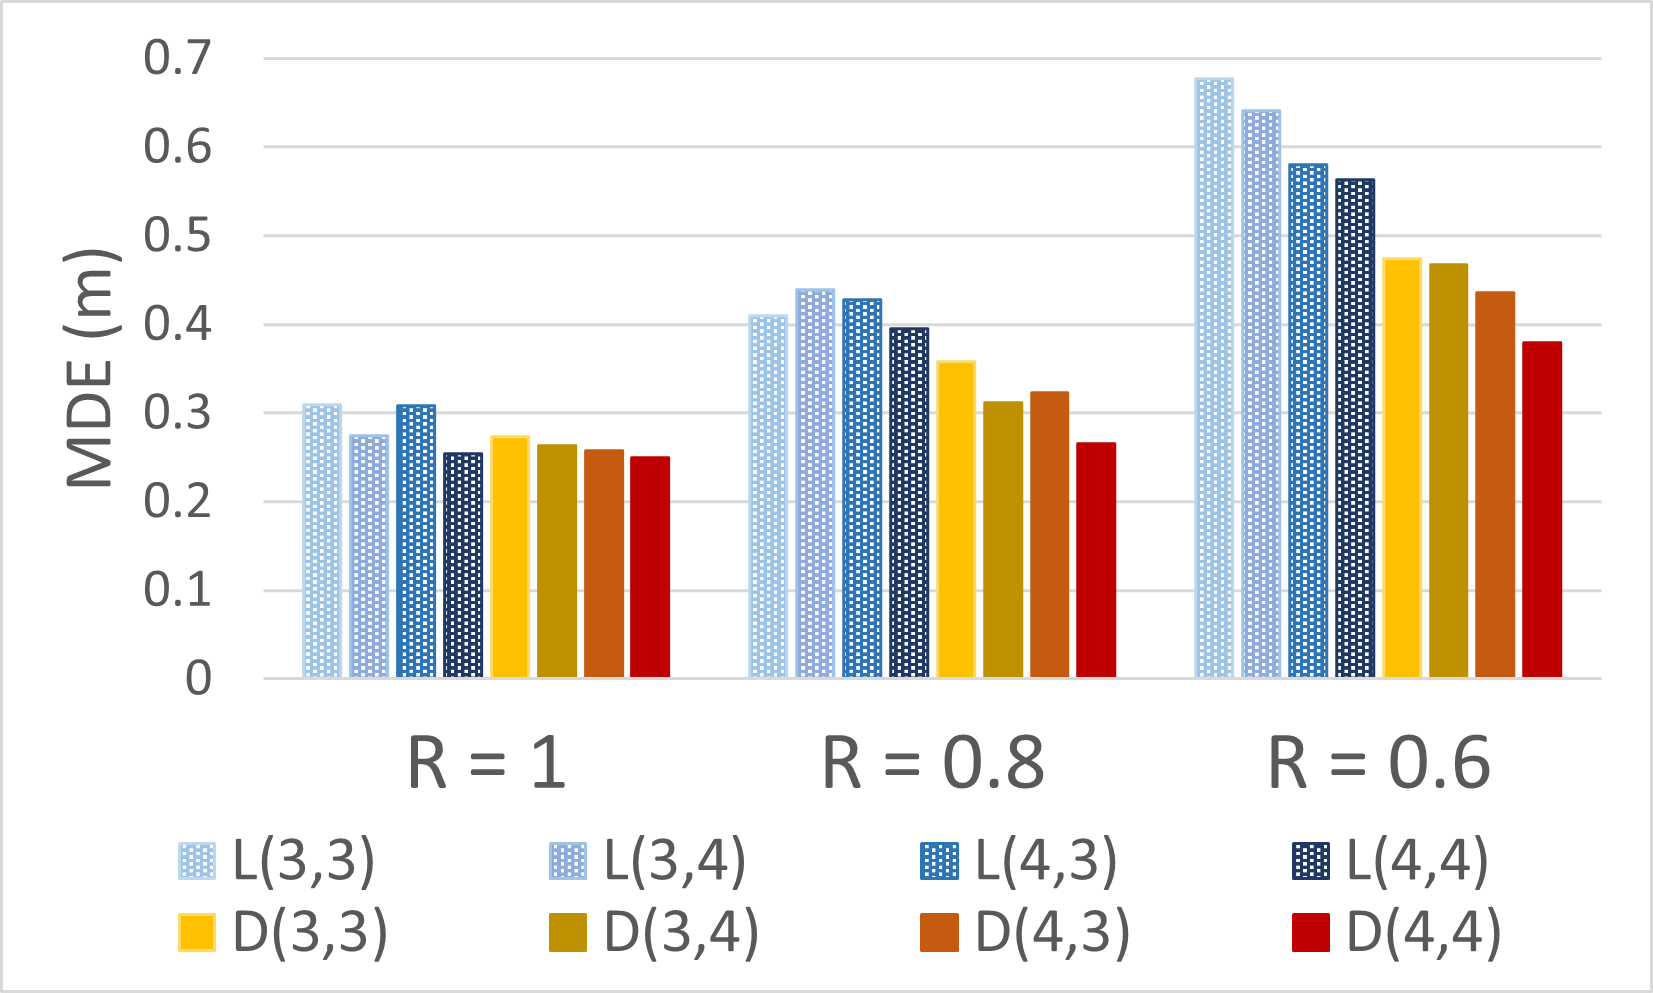
\includegraphics[width=0.8\textwidth]{images/5_6_Blocked_Object_MDE_SW.png}
        \caption{MDEs of scripted walk}
        \label{figure:5_6_Blocked_Object_MDE_SW}
    \end{subfigure}
    %\caption{.}
% subfigs for free walk
    % \centering
    \begin{subfigure}{1\linewidth}
    \centering
        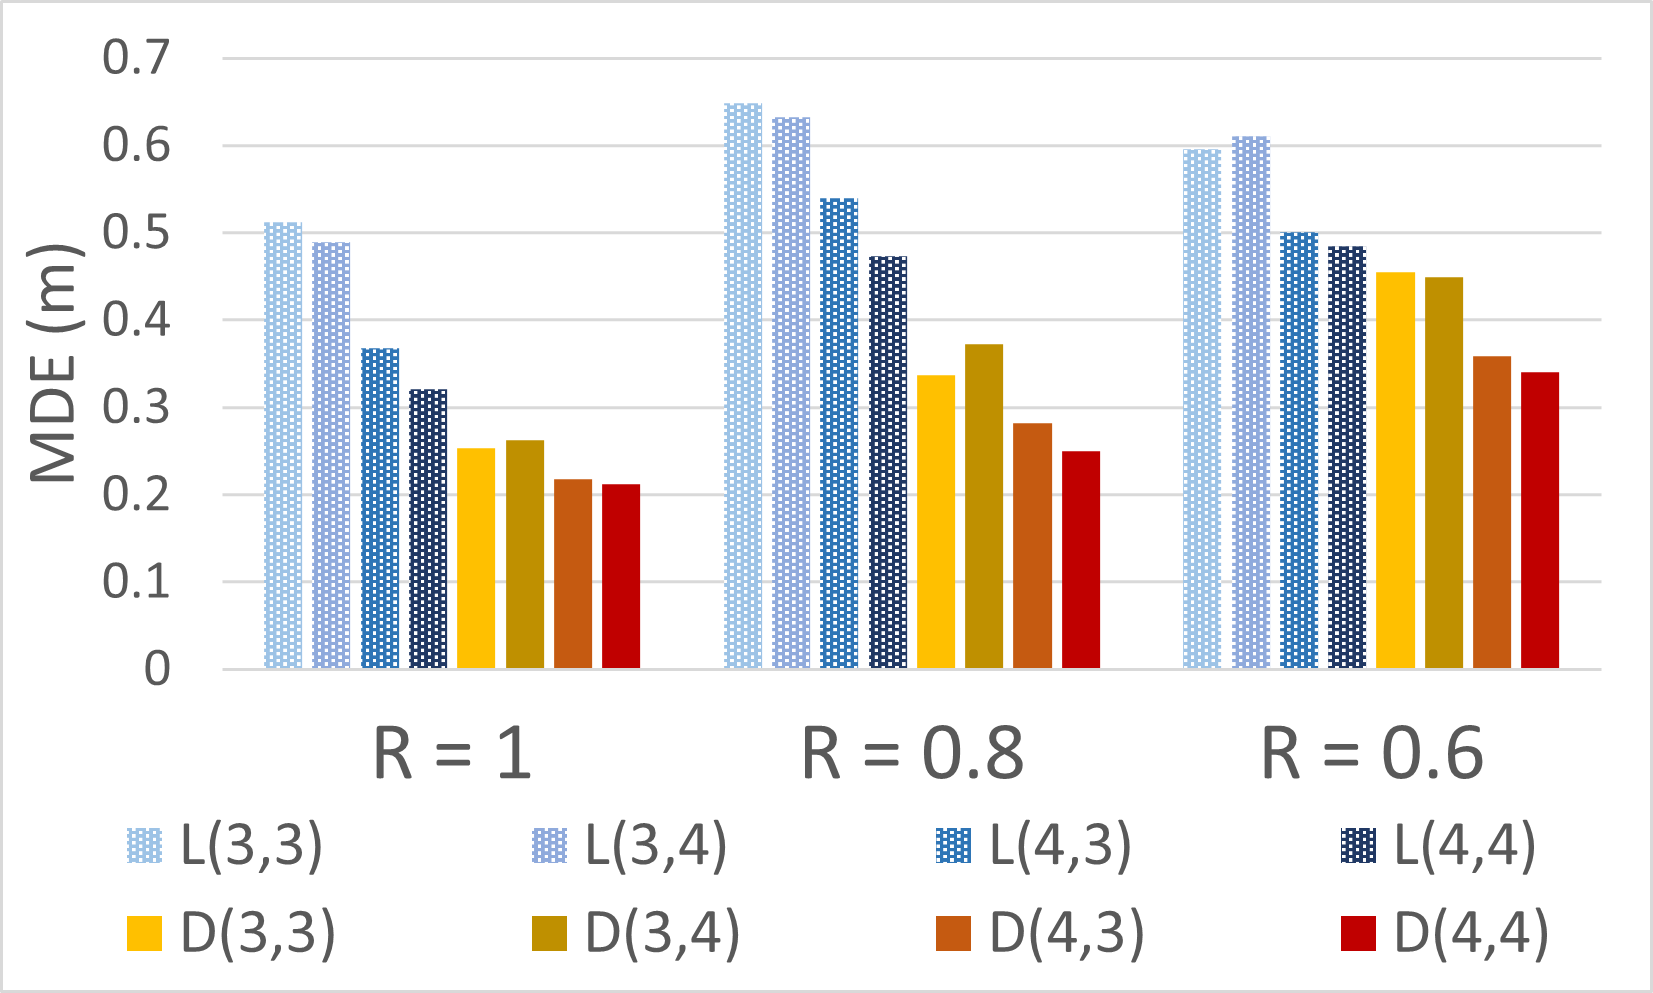
\includegraphics[width=0.8\textwidth]{images/5_6_Blocked_Object_MDE_FW.png}
        \caption{MDEs of free walk}
        \label{figure:5_6_Blocked_Object_MDE_FW}
    \end{subfigure}
\caption{MDEs of each scenario with different blocked object rate R.}
\label{figure:5_6_Blocked_Object_MDE}
\end{figure}
%=== figure === %

%*----------------------section 5.7
\section{Effects of the Number of Beacons}

\subsection{Setup}

\paragraph{}
Wireless hash localization in our system is very dependent on the wireless signals sent by the beacons deployed in the environment. However, the number of beacons can be affected by beacon failures or environmental deployment constraints. Therefore, this section discusses the impact of different numbers of beacons on positioning. 

\paragraph{}
We explore the effect of different numbers of beacons on positioning by changing the number of beacons deployed in the environment. Fig.~\ref{figure:5_7_Number_of_Beacons_Setup} shows the deployment of different number of beacons.

%=== figure 5_7_Number_of_Beacons_Setup=== %
\begin{figure}[tbph]
    \begin{center}
    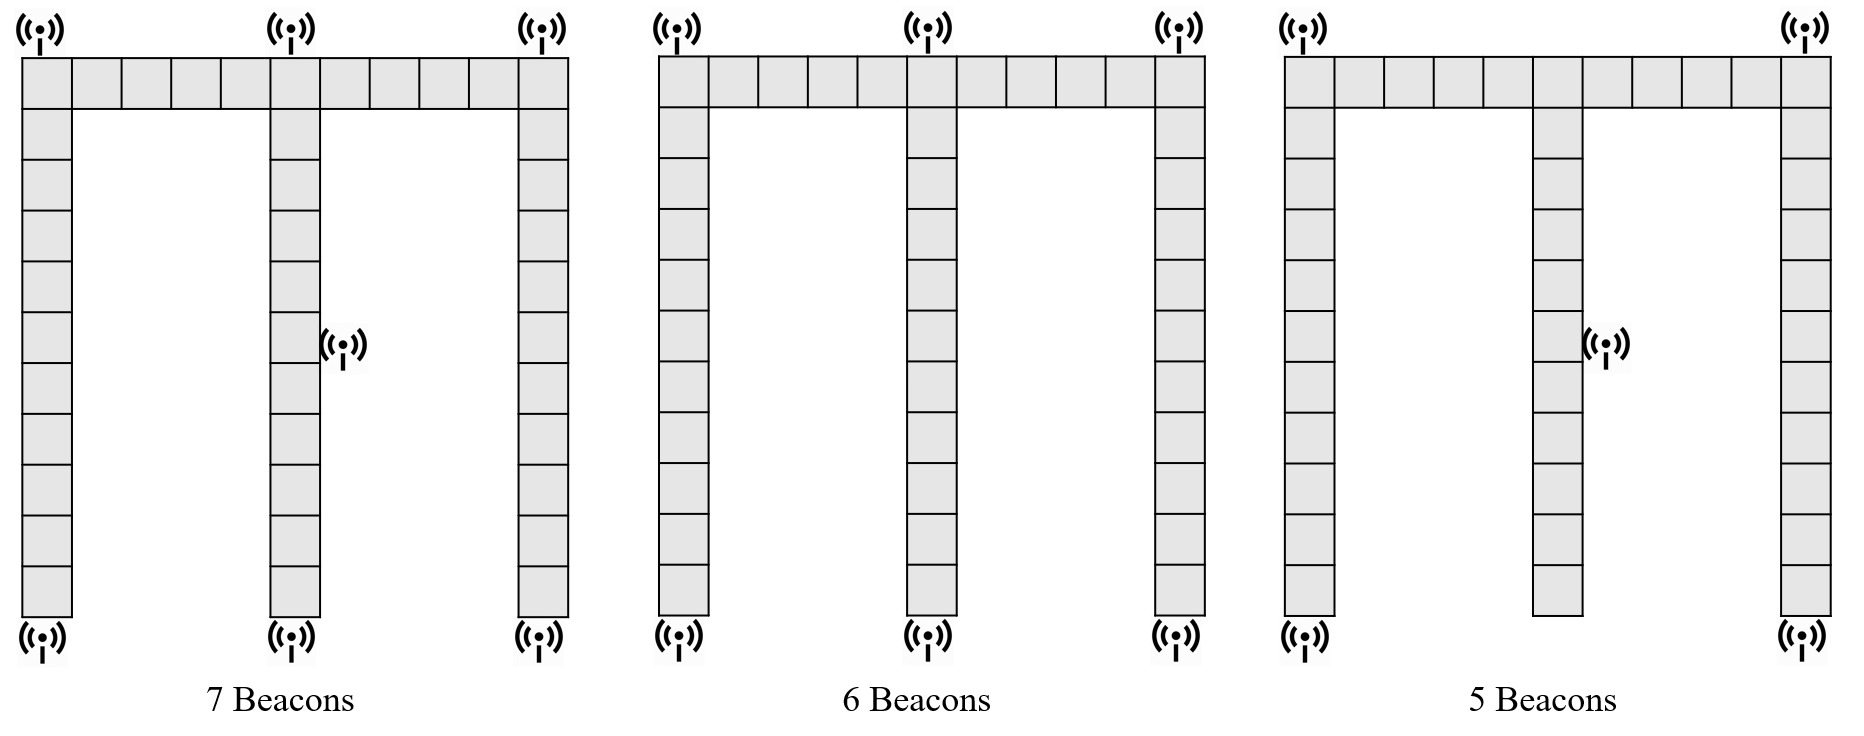
\includegraphics[width=0.85\textwidth]{images/5_7_Number_of_Beacons_Setup.png}
    \caption{Deployment of different number of beacons.}
    \label{figure:5_7_Number_of_Beacons_Setup}
    \end{center}
\end{figure}
% === figure === %

\subsection{Results}

\paragraph{}
The experimental results are shown in Fig.~\ref{figure:5_7_Number_of_Beacons_MDE}. Both $BTrack$ and $JoLo$, which use pure wireless signals, have increased MDEs due to the decrease in the number of beacons. Because $Lin$ and $DyLo$ are assisted by image data, the overall MDEs are better than $BTrack$ and $JoLo$. The reason why the MDE of $DyLo$ increases more than $Lin$ is that image hash positioning of $DyLo$ relies on wireless filtering to a certain extent. Therefore, when the performance of wireless hash positioning decreases due to the decrease in the number of beacons, the overall performance also decreases. However, the number of beacons is easy to increase due to the low cost of the beacon.

%=== figure 5_7_Number_of_Beacons_MDE=== %
% subfigs for scripted walk
\begin{figure}[tbph]%\ContinuedFloat
    %\centering
    \begin{subfigure}{1\linewidth}
    \centering
        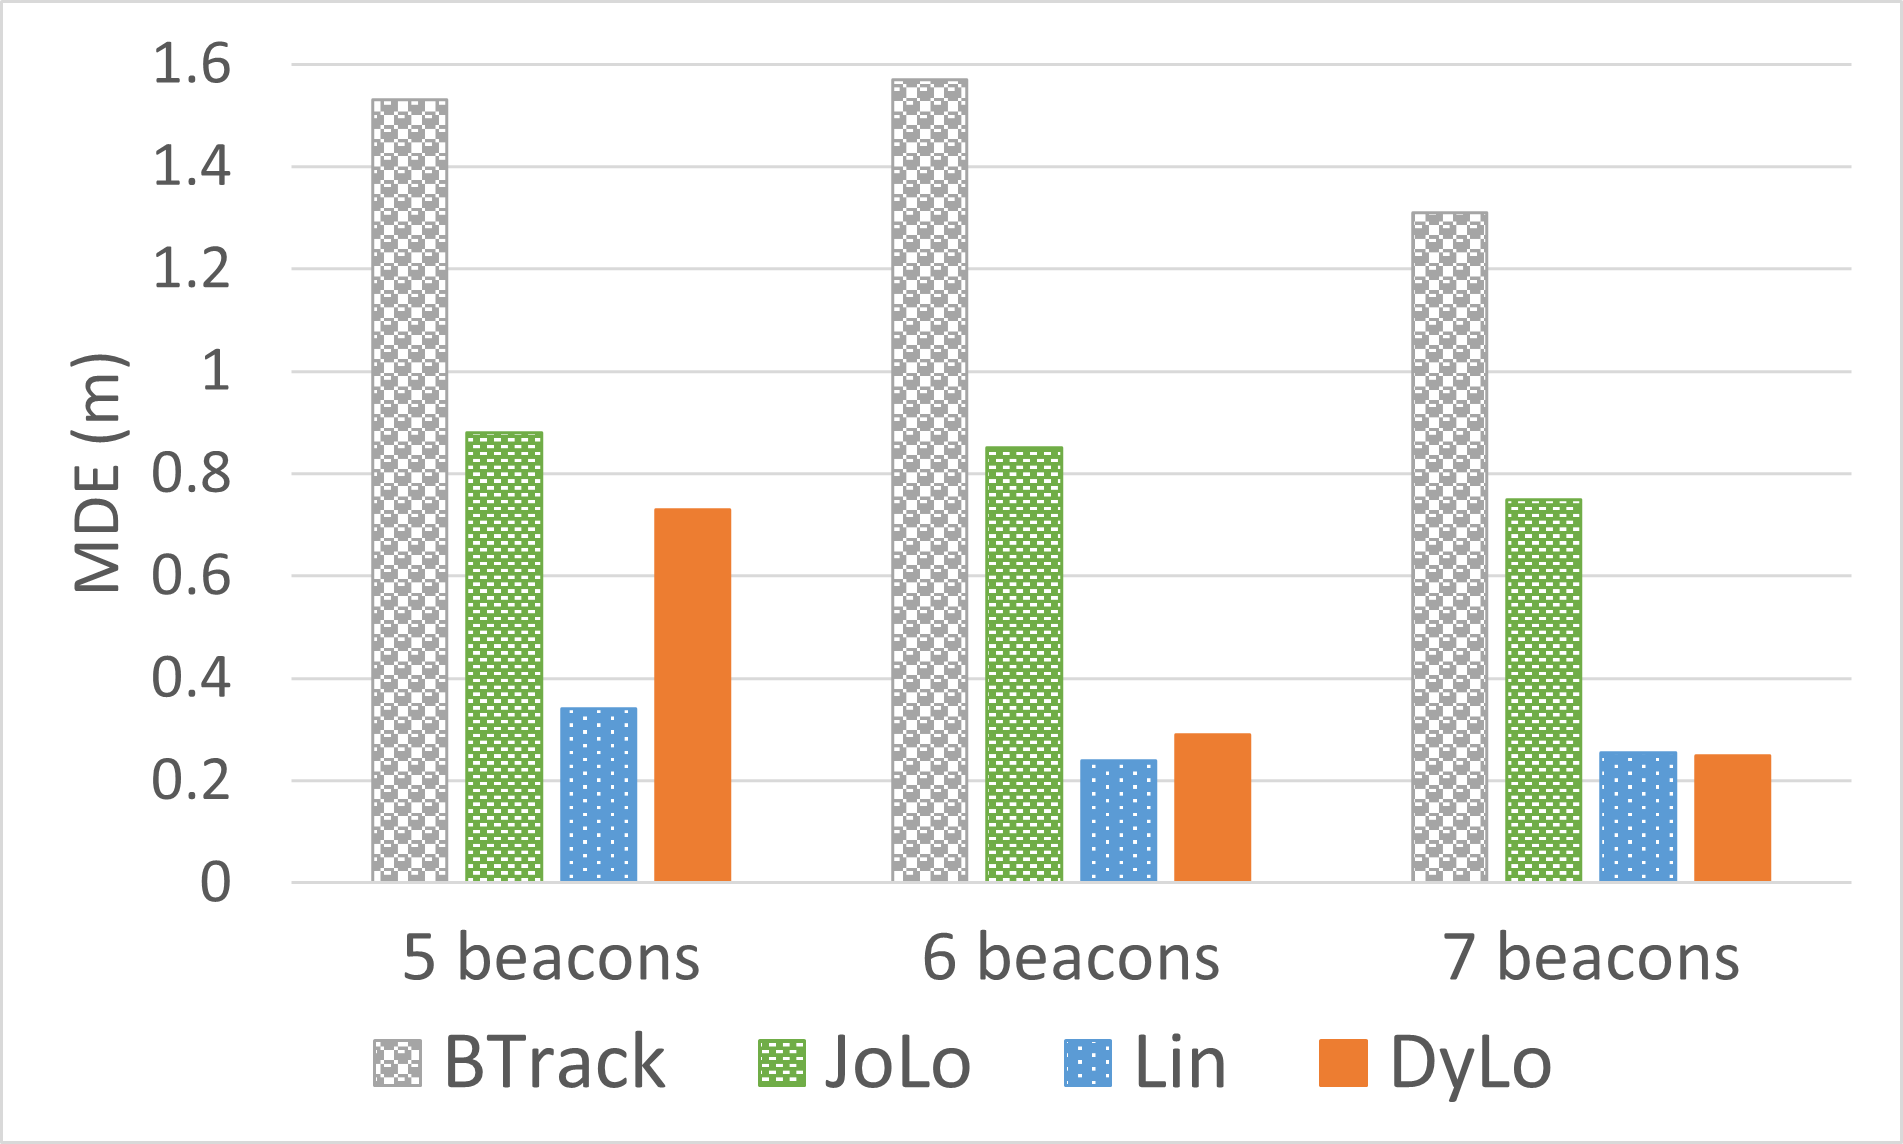
\includegraphics[width=0.8\textwidth]{images/5_7_Number_of_Beacons_MDE_SW.png}
        \caption{MDEs of scripted walk}
        \label{figure:5_7_Number_of_Beacons_MDE_SW}
    \end{subfigure}
    %\caption{.}
% subfigs for free walk
    % \centering
    \begin{subfigure}{1\linewidth}
    \centering
        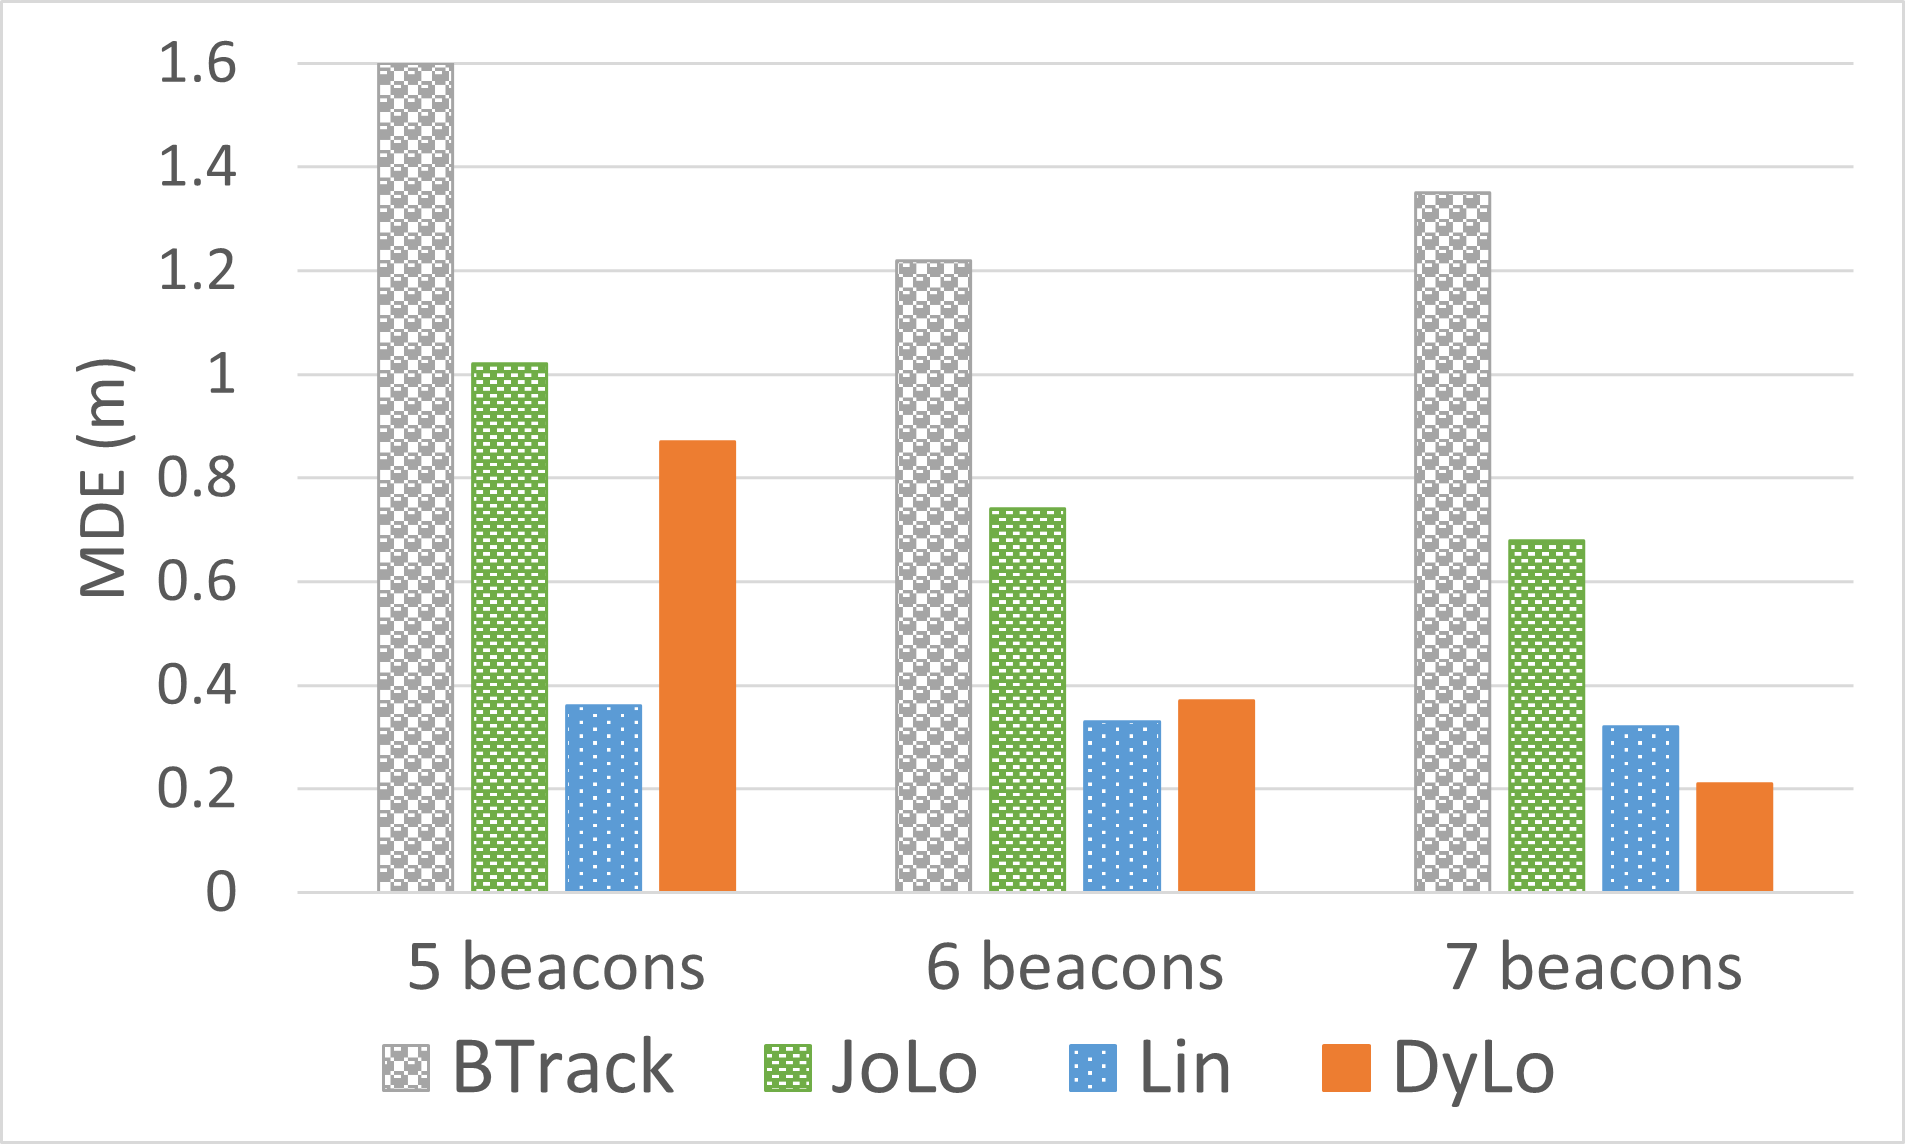
\includegraphics[width=0.8\textwidth]{images/5_7_Number_of_Beacons_MDE_FW.png}
        \caption{MDEs of free walk}
        \label{figure:5_7_Number_of_Beacons_MDE_FW}
    \end{subfigure}
\caption{MDEs of each scenario with different number of beacons.}
\label{figure:5_7_Number_of_Beacons_MDE}
\end{figure}
%=== figure === %

%*----------------------section 5.8
\section{Effects of Device Heterogeneity}

\subsection{Setup}

%paragraph 
\paragraph{}
The wireless signals used in wireless hash localization are received by mobile devices. However, different devices will affect the success rate of signal reception due to the hardware design of chips and antennas. Therefore, this chapter will explore the effect of heterogeneity between devices on wireless signal reception.

\paragraph{}
We ignore some received packets in testing wireless signals randomly to simulate this situation. The packet reception rate will be used to calculate the ratio of BLE packets loss, which is calculated as
%---
\begin{equation}
\label{equation:Packet_Reception_Rate}
Packet\ Reception\ Rate\ = \frac{Packets\ received\ by\ the\ device}{All\ packets\ sent\ by\ BLE\ beacon}
\end{equation}
%---

\paragraph{}
In the experiment, we divided into three groups: $G$, the packet reception rate of each device is the best; $G^`$, the packet reception rate of one device Sharp V is reduced to 41.5\%, and the remaining three devices remain the best; $G^{``}$, the packet reception rate of the device Sharp V is reduced to 41.5\%, the packet reception rate of the device hTC U19e is reduced to 41.8\%, and the remaining two devices remain the best. Evaluate the effect of device heterogeneity on the overall localization system by observing the MDE changes of the three groups of $G$, $G^`$, $G^{``}$. The packet reception rate relationship between the three groups of devices is arranged in Table~\ref{table:5_8_Packet_Receiving_Capabilities}.

% === table === %
\begin{table}
    \begin{center}
    \caption{Packet receiving capabilities of wireless devices groups}
    \label{table:5_8_Packet_Receiving_Capabilities}
        \begin{tabular}{|c|c|c|c|}
            \hline
                & \multicolumn{3}{|c|}{Packet Reception Rate} \\
            \hline
                Device & $G$ & $G^`$ & $G^{``}$\\
            \hline
                Samsung A51 & 99.1\% & 99.1\% & 99.1\%\\
            \hline
                hTC U11     & 99.3\% & 99.3\% & 99.3\%\\
            \hline
                hTC U19e    & 99.8\% & 99.8\% & 41.8\%\\
            \hline
                Sharp V     & 99.8\% & 41.5\% & 41.5\%\\
            \hline
        \end{tabular}
    \end{center}
\end{table}
% === table === %

\subsection{Results}

\paragraph{}
The experimental results are shown in Fig.~\ref{figure:5_8_Device_Heterogeneity_MDE}. When $DyLo$ simply uses wireless signals to locate ($DyLo(W)$), it will be affected by device heterogeneity and then increase MDEs like $JoLo$. However, after adding image data, the dynamic weighting between wireless hash and image hash makes $DyLo$ better than $JoLo$ with pure wireless signals. The reason why the MDE of $DyLo$ increases more than $Lin$ is that image hash positioning of $DyLo$ relies on wireless filtering to a certain extent. Therefore, when the performance of wireless hash positioning decreases due to the decrease in the number of beacons, the overall performance also decreases.
%

%=== figure 5_8_Device_Heterogeneity_MDE=== %
% subfigs for scripted walk
\begin{figure}[tbph]%\ContinuedFloat
    %\centering
    \begin{subfigure}{1\linewidth}
    \centering
        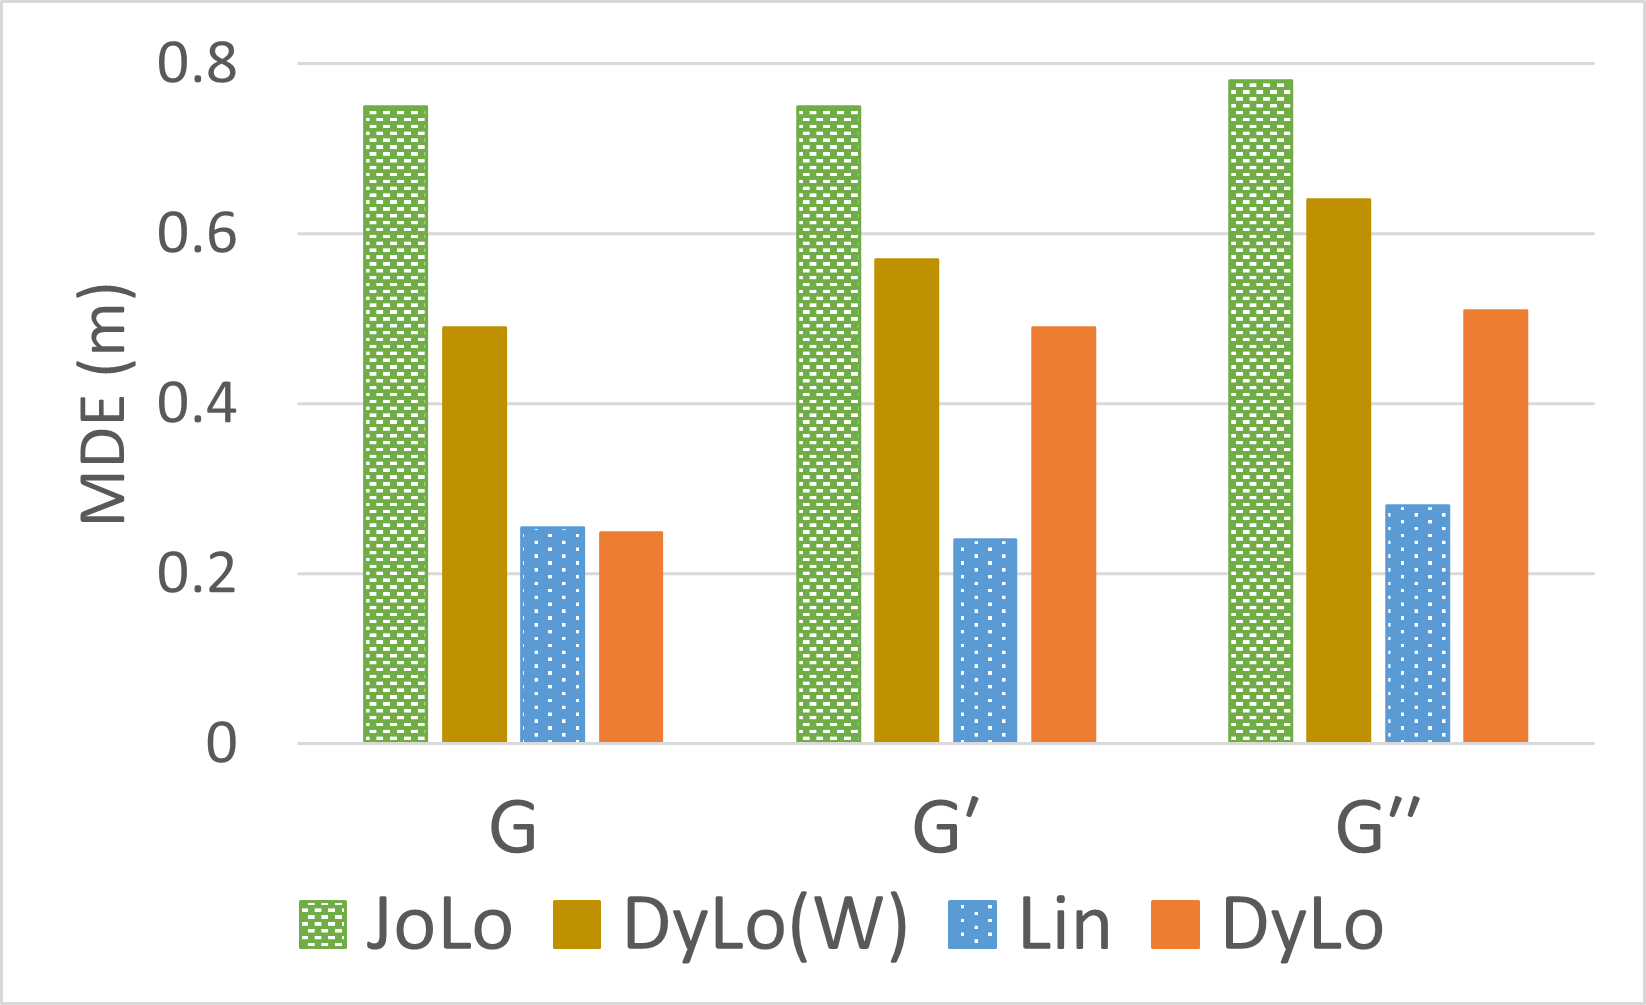
\includegraphics[width=0.8\textwidth]{images/5_8_Device_Heterogeneity_MDE_SW.png}
        \caption{MDEs of scripted walk}
        \label{figure:5_8_Device_Heterogeneity_MDE_SW}
    \end{subfigure}
% subfigs for free walk
    % \centering
    \begin{subfigure}{1\linewidth}
    \centering
        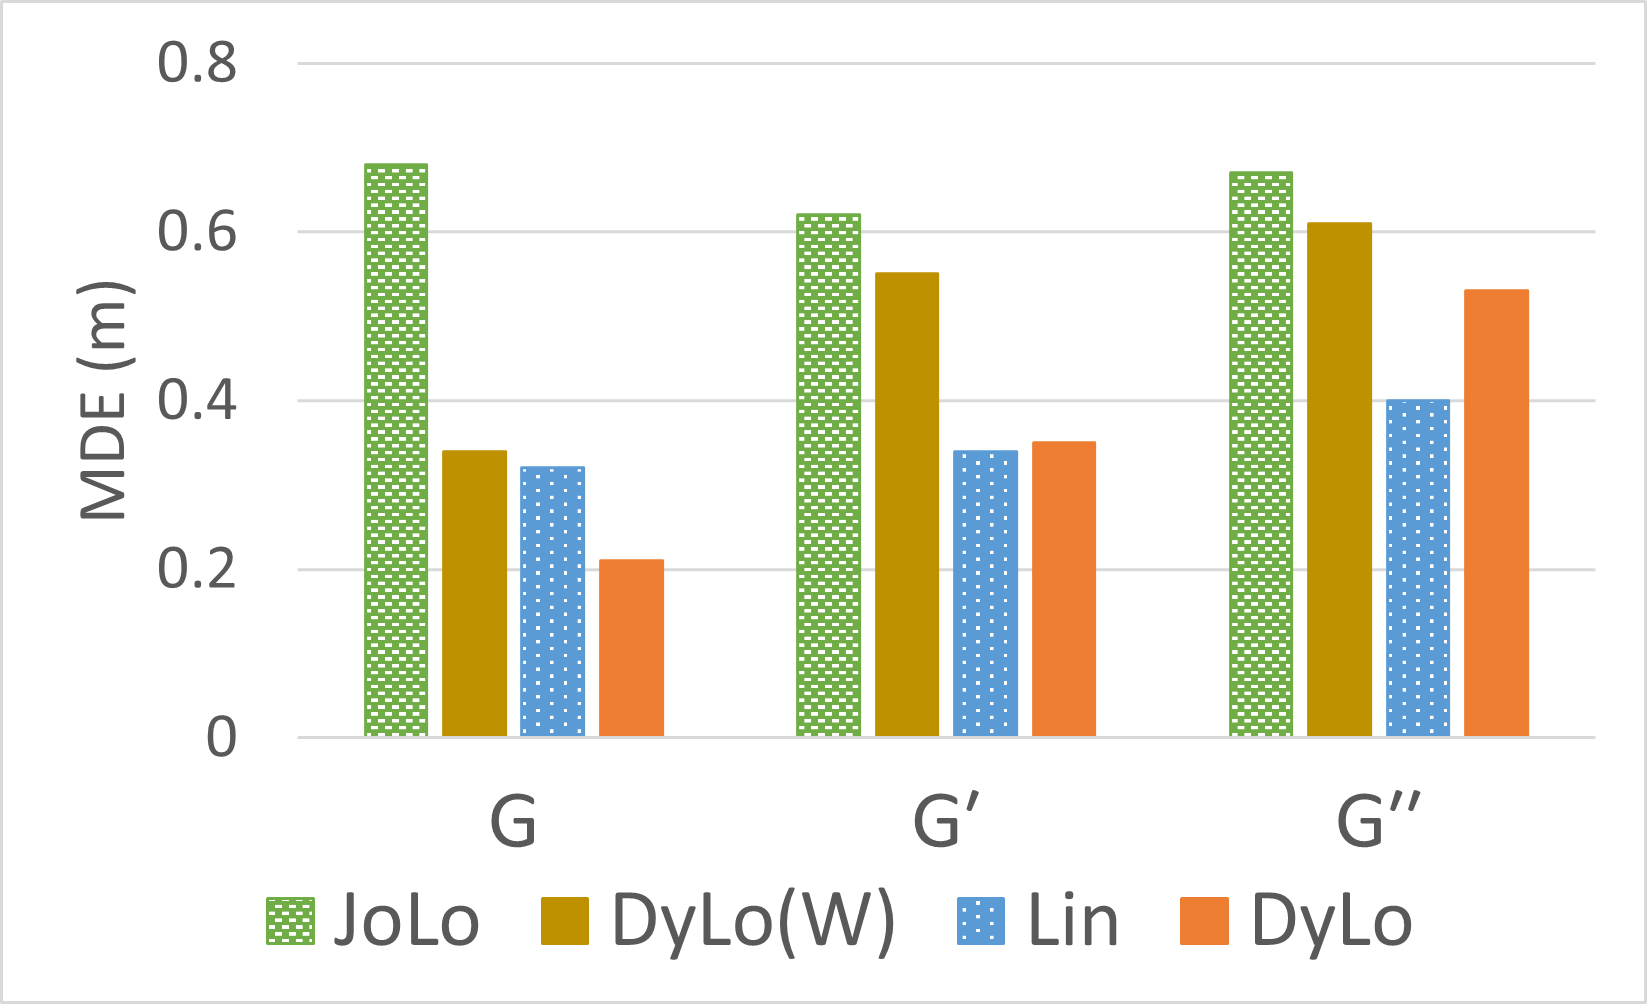
\includegraphics[width=0.8\textwidth]{images/5_8_Device_Heterogeneity_MDE_FW.png}
        \caption{MDEs of free walk}
        \label{figure:5_8_Device_Heterogeneity_MDE_FW}
    \end{subfigure}
\caption{MDEs of each scenario with different packet receiving capabilities.}
\label{figure:5_8_Device_Heterogeneity_MDE}
\end{figure}
%=== figure === %


%*------------------------------------------------chapter 6-------------------------------------------
\chapter{Conclusion}

%paragraph
\paragraph{}
In this paper, we propose a dynamic indoor localization system based on wireless signals and image data collected from mobile devices. Also, our system converts wireless signals into wireless hash and image data into image hash. Second, data preprocessing and enhancing are applied for wireless hash to solve the discreteness of the RSSI data. Moreover, we combine wireless and image phases dynamically to improve the localization accuracy by taking advantage of each. Finally, we use dynamic weighting for particle filter to deal with immediate changes in the performance in wireless and image phases.
%

%paragraph
\paragraph{}
We do experiments in two different-sized offices, and the experimental results show that our system reduces localization errors to less than 0.25 meters. This accuracy outperforms at least 34\% than the positioning method based on wireless and image fingerprint, and at least 69\% than the positioning method only based on wireless fingerprint. Furthermore, our system has outstanding performance for irregular paths.
%
   
%*------------------------------------------------------

\addcontentsline{toc}{chapter}{Bibliography}
\bibliographystyle{IEEEtran}
\bibliography{references}

\end{document}
